\documentclass[12pt, letterpaper]{article}
\usepackage{graphicx} % Required for inserting images
\usepackage{hyperref}
\usepackage{listings}
\usepackage{amssymb}
\usepackage{amsmath}
\usepackage[english]{babel}
\usepackage{nicefrac, xfrac}
\usepackage{mathtools}
\usepackage[table,xcdraw]{xcolor}
\definecolor{light-gray}{gray}{0.95}
\definecolor{sap}{RGB}{130, 36, 51}
\definecolor{newBlue}{RGB}{0, 109, 199}
\definecolor{lg}{RGB}{102, 161, 95}
\definecolor{g}{RGB}{60, 50, 50}
\usepackage[paper=a4paper,left=20mm,right=20mm,bottom=25mm,top=25mm]{geometry}
\newcommand{\code}[1]{\colorbox{light-gray}{\texttt{#1}}}
\newcommand{\shelll}[1]{\colorbox{black}{\textcolor{white}{\texttt{#1}}}}
\newcommand{\shell}[1]{\colorbox{black}{\textcolor{white}{\texttt{casufrost@debian:$\sim$\$ #1}}}}
\newcommand{\codee}[1]{\colorbox{white}{\texttt{#1}}}
\newcommand{\acc}{\\\hphantom{}\\}
\newcommand{\dete}{{\rightarrow}}
\newcommand{\fdot}{{\(\bullet\) }}
\newcommand{\comm}[1]{\color{lg}\textit{\hphantom{spaz}// \text{#1}}\color{black}}
\newcommand{\textg}[1]{\color{g}{\textbf{#1}}\color{black}}
\newcommand{\boxedMath}[1]{\begin{tabular}{|c|}\hline \texttt{#1} \\ \hline\end{tabular} :}
\newcommand\greybox[1]{%
  \vskip\baselineskip%
  \par\noindent\colorbox{light-gray}{%
    \begin{minipage}{\textwidth}#1\end{minipage}%
  }%
  \vskip\baselineskip%
}
\title{Reti di Elaboratori}
\author{Marco Casu}
\date{\vspace{-5ex}}
\begin{document}



\maketitle
\begin{figure}[h]
    \centering{
        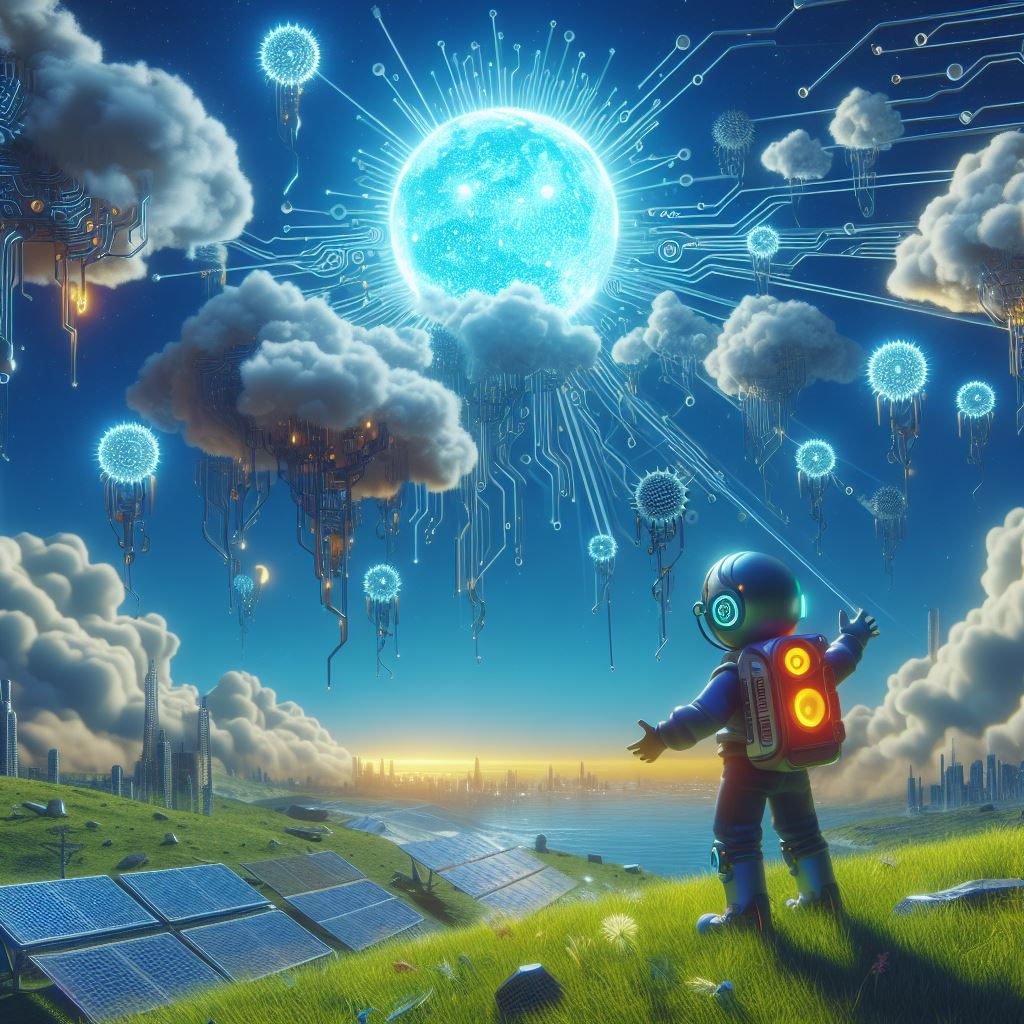
\includegraphics[width=1\textwidth ]{images/cop.jpg}
    }
\end{figure}
\newpage
\tableofcontents
\newpage
\section{Reti di Calcolatori e Internet}
Cos'è una richiesta di rete? E soprattutto quali sono i passaggi ed il procedimento scaturito a seguito di una richiesta? Questo corso
si concentrerà sull'aspetto del \textit{networking}, ossia, su come avviene la comunicazione tramite più elaboratori.\acc
Una \textit{connessione} è una comunicazione aperta in cui sono coinvolte entrambe le parti in attesa di ricevere ed inviare
messaggi, tramite l'apertura di un \textit{socket} (si approfondirà in seguito). Il problema di una comunicazione di questo tipo,
è il bisogno di avere la certezza che i messaggi inviati da una parte siano ricevuti correttamente dall'altra, senza il rischio di
comunicare "a vuoto", per questo sono definiti degli appositi protocolli.\acc
\textbf{Host} : Un dispositivo connesso alla rete in modo periferico, non funge da esclusivo tramite per la comunicazione,
ed è un sistema "periferico", esegue delle \textit{app} che forniscono servizi sulla rete.\acc
\textbf{Switch} : Gli switch sono i dispositivi capaci di "instradare" i \textit{pacchetti}.\acc
\textbf{Rete} : Una collezione di dispositivi host/switch e collegamenti gestiti da un unico ente/organizzazione.\begin{center}
    \includegraphics[width=1\textwidth ]{images/reteDef.eps}
\end{center}
Quella che noi chiamiamo \textbf{internet}, è una "\textit{rete di reti}", ossia l'insieme interconnesso di tutte le reti
pubbliche, che si stabilisce e necessita di protocolli su tutti i livelli : \begin{itemize}
    \item Livello di applicazione
    \item Livello di trasporto
    \item Livello network
    \item Livello di collegamento
\end{itemize}
Lo scopo di internet è quello di essere un infrastruttura che fornisce i servizi alle applicazioni distribuite, è
un interfaccia di programmazione e fornisce un servizio di \textit{trasporto dei dati}.\acc
Un \textbf{protocollo di rete}, stabilisce delle regole riguardanti lo scambio di messaggi, con le relative "azioni" specifiche
da intraprendere per la ricezione di messaggi ed eventi, definiscono il \textit{formato} e \textit{l'ordine} dei messaggi
da inviare fra le entità di rete, e le azioni intraprese sulla ricezione e trasmissione dei messaggi.
\subsection{Struttura di Internet e Link}
Una rete è quindi un insieme di nodi collegati tramite dei \textit{link}, composta da dispositivi di interconnessione, che
si scambiano informazioni, usualmente utilizziamo il termine \textit{host} per i dispositivi che usufruiscono di un servizio,
e \textit{server} per i dispositivi che lo erogano.\acc
I dispositivi di interconnessione, ricevono un segnale, lo modificano e lo ritrasmettono, sono i \textit{router} (collegano una
rete ad altre reti) e gli  \textit{switch} (collegano più dispositivi ad una rete locale). I collegamenti, o link, possono
essere cablati (rame o fibra ottica) oppure wireless, senza cavi (onde elettromagnetiche).\acc
Le reti locali come quelle casalinghe o aziendali, si collegano ad una rete regionale ISP (internet service provider) di router interconnessi detta
\textit{core} o \textit{backbone}, che a sua volta si collega ad una simile struttura ma a livello nazionale o globale.\acc
\subsubsection{Reti Cablate e Wireless}
Nell'accesso via cavo, c'è un terminale comune per più abitazioni detto \textbf{CMTS}, ossia \textit{Cable Modem Termination System},
che viene poi diramato nelle diverse abitazioni, i dati dalla rete ed i segnali per la televisione sono trasmessi sul medesimo
cavo ma a frequenze differenti. Il CMTS è direttamente collegato ad un ISP. In questo modello diverse case condividono la rete di
accesso.\begin{center}
    \includegraphics[width=1.1\textwidth ]{images/cableHeadend.eps}
\end{center}
La \textbf{DSL} diversamente, utilizza la linea telefonica esistente, collegandosi alla DSLAM, i dati sulla linea
DSL vanno su internet, la voce su DSL va sulla linea telefonica. \acc
In una rete \textit{domestica}  c'è un \textit{modem}
(si occupa di ricevere il segnale analogico e di  \textit{modularlo} in segnale digitale)
connesso ad un CMTS, collegato via cavo ad
un router, collegato direttamente tramite \textit{Ethernet} agli host, oppure collegato ad un \textit{access point WI-FI} che
permette la connessione senza fili, questi ultimi tre molto spesso sono combinati in un unico device.\acc
La connessione senza fili, o wireless connette i sistemi terminali (host) al router, tramite il già citato
access point, esistono reti locali senza fili (WLAN), che hanno una copertura di circa 30 metri, e reti di accesso
cellulare \textit{wide area}, utilizzate dai dispositivi mobili e fornite da un operatore di rete cellulare, ed hanno una
copertura più ampia, nell'ordine dei kilometri.\acc
Le reti aziendali, come quelle delle università sono di una scala diversa rispetto quelle domestiche, prevedono molti più
dispositivi, ed un mix di varie tecnologie di collegamento, cablate o wireless, tramite svariati switch e router.
\subsubsection{Comunicazione e Classificazione delle Reti}
Un host comunica tramite l'invio e la ricezioni di messaggi da un applicazione sottoforma di \textit{pacchetti} di dati, ossia
messaggi suddivisi in blocchi più piccoli, di lunghezza $L$ bit. L'host trasmettono i pacchetti nella rete
ad una \textit{velocità di trasmissione} di $R$ $\nicefrac{bit}{sec}$. Il \textit{ritardo} di trasmissione del pacchetto è
il tempo necessario per trasmettere il pacchetto ($L$ bit) nel collegamento, ed equivale a $\dfrac{L}{R}$ secondi.\acc
Il segnale si propaga fra trasmettitore e ricevitore, tramite \textit{supporti guidati}, ossia i mezzi solidi (cavi), oppure
\textit{non guidati}, propagandosi liberamente nell'aria (onde elettromagnetiche).\begin{itemize}
    \item Il \textbf{cavo coassiale} è provvisto di due conduttori di rame concentrici, è bidirezionale, supporta più canali
          date diverse frequenze, ed è resistente alle interferenze.
    \item La \textbf{fibra ottica} ha soppiantato il cavo coassiale, è una fibra di vetro che trasporta impulsi luminosi, dove ciascun
          impulso rappresenta un bit, la luce rimbalza nel cavo muovendosi ad alta velocità, è necessario però considerare dei
          ripetitori (anche se molto distanziati), dato che la luce rimbalzando potrebbe tendere a disperdersi causando una perdita
          di informazioni.
    \item La rete \textbf{wireless} non ha un supporto guidato, il segnale è propagato nell'aria, è quindi \textit{broadcast},
          chiunque può ricevere il segnale. Tale metodo di comunicazione è \textit{half-duplex}, ossia, la comunicazione avviene da un
          mittente ad un destinatario, e non è possibile comunicare fra due enti contemporaneamente, è soggetta ad effetti dovuti all'ambiente
          di propagazione, come interferenze, riflessione e ostruzione da parte di oggetti fisici.
\end{itemize}
Esiste una scala di classificazione delle reti :\begin{center}
    \begin{tabular}{|
            >{\columncolor[HTML]{EFEFEF}}c |
            >{\columncolor[HTML]{FFFFFF}}c |c|
            >{\columncolor[HTML]{FFFFFF}}c |}
        \hline
        \cellcolor[HTML]{9AFF99}{\color[HTML]{000000} Scala} & \cellcolor[HTML]{9AFF99}Tipo & \cellcolor[HTML]{9AFF99}Nome completo & \cellcolor[HTML]{9AFF99}Esempio \\ \hline
        Distanza ravvicinata                                 & PAN                          & Personal Area Network                 & Bluetooth                       \\ \hline
        Edificio                                             & LAN                          & Local Area Network                    & WiFi, Ethernet                  \\ \hline
        Città                                                & MAN                          & Metropolitan Area Network             & Cablata, DSL                    \\ \hline
        Paese                                                & WAN                          & Wide Area Network                     & Grandi ISP                      \\ \hline
        Pianeta                                              & Internet                     & La rete di tutte le reti              & L'Internet                      \\ \hline
    \end{tabular}
\end{center}
La \textbf{LAN} è la rete locale, come una rete domestica, è una rete privata ed ogni terminale connesso ad essa è identificato
da un indirizzo distinto dagli altri, può essere a \textit{cavo condiviso} oppure a \textit{commutazione} con uno switch.\begin{center}
    \includegraphics[width=1\textwidth ]{images/cavocondiviso.eps}
\end{center}
In tale modello di cavo condiviso il pacchetto inviato ad un dispositivo viene ricevuto da tutti, solo il destinatario lo
elaborerà, tutti i restanti host lo ignoreranno.\acc \begin{center}
    \includegraphics[width=0.7\textwidth ]{images/commutazione.eps}
\end{center}
Quest'ultimo a commutazione è il più utilizzato tutt'oggi, ogni dispositivo è direttamente collegato allo switch, ed esso è
in grado di riconoscere gli host ed inviare i pacchetti esclusivamente al destinatario, riduce il traffico nella LAN.\acc
Le reti \textbf{WAN} sono reti geografiche, vengono interconnessi dispositivi di comunicazione, necessari a città, regioni o
perfino nazioni. I dispositivi in questione sono switch, router e modem, tale rete è gestita da un grande operatore/ente di
telecomunicazioni detto IPS (Internet Service Provider) che fornisce i servizi alle organizzazioni.\acc Una WAN può vedere i suoi
dispositivi di comunicazione connessi punto-punto, oppure a commutazione, con più punti di terminazione (usata nelle dorsali di
Internet), tutt'oggi è raro trovare LAN o WAN isolate, spesso sono connesse fra loro per formare una internetwork (internet), per
mettere in comunicazione due LAN in città differenti tramite una WAN.\begin{center}
    \includegraphics[width=1\textwidth ]{images/internetwork.eps}
\end{center}
\subsubsection{Nucleo della Rete} \label{NucleoRete}
Si definisce nucleo della rete, quella parte composta esclusivamente da router  che effettuano \textit{commutazione} di pacchetto, ossia
ricevono il pacchetto, e lo re-indirizzano tramite i collegamenti. Ogni router presenta più porte, si occupa di fare il
cosiddetto \textbf{forwarding}, ossia l'azione locale di spostare i pacchetti in arrivo dal collegamento in ingresso, al collegamento
in uscita, è un azione locale del router.\acc
Il \textbf{routing} invece è un azione globale, si intende la determinazione dei percorsi origine-destinazione che i pacchetti
dovranno prendere all'interno dell'Internet, tale decisione è presa tramite degli algoritmi di instradamento.\acc
Con il termine \textit{Trasmissione}, si intende l'azione che intraprende un pacchetto per essere trasferito interamente
sul collegamento. Tale termine non include l'intero tragitto fino a destinazione, ma esclusivamente la (appunto) trasmissione sull'eventuale
cavo, il \textit{ritardo di trasmissione} è quindi il delay misurato in secondi per trasmettere un pacchetto, si è già specificato che tale
valore è uguale a $\dfrac{L}{R}=\dfrac{\text{bit di un pacchetto}}{\text{bit per secondo}}$.\acc
I router funzionano nella seguente maniera, detta \textbf{store and forward} : Un pacchetto deve arrivare per intero ad un router
prima di essere ri-trasmesso su un nuovo collegamento.\begin{quote}
    \color{gray} \textit{Esempio} : Si devono trasferire, dal collegamento A al collegamento B, 3 pacchetti da 10 Kbit ad una
    velocità di 100 Mbit per secondo, si assume che il  tempo che impiega un bit per propagarsi nel collegamento è zero.
    In totale, il ritardo di trasmissione sarà : $\dfrac{10*3*10^3}{100*10^6}=\dfrac{3}{100*10^2}=\dfrac{3}{10^4}=0,0003\text{ sec }=0,3\text{ msec }$
    \color{black}
\end{quote}
Un problema noto durante la tramissione dei pacchetti è l'\textbf{accodamento}, avviene quando la velocità di arrivo ad
un router da parte di un link è maggiore della velocità di trasmissione in uscità (dal link al router), quindi si causa un
accodamento in attesa della trasmissione.\begin{center}
    \includegraphics[width=0.7\textwidth ]{images/accodamento.ip.eps}
\end{center}
I pacchetti arrivano al router prima di essere trasmessi sul link, quindi si accoderanno in una memoria interna del router prima
di essere ritrasmessi, se i pacchetti accodati diventano troppi e la memoria viene esaurita, ci sarà una \textit{perdita} di
pacchetti. \acc
Una possibile soluzione alla perdita è la \textbf{commutazione di circuito}, ossia, far si che i diversi host non condividano lo
stesso collegamento per i pacchetti, bensì, si considerano dei canali riservati per la comunicazione tra sorgente e destinazione.\acc
Non c'è condivisione, ci saranno quindi svariati collegamenti, in numero necessario per permettere a tutti i dispositivi di
poter comunicare in modo libero, ovviamente non tutti comunicano nello stesso momento, quindi i un segmento di cirucito potrebbe
rimanere inutilizzato.\acc
Un'altra alternativa è quella di condividere lo stesso circuito, riservando ad ogni comunicatore una frequenza (\textit{FDM}), oppure un certo
quanto temporale (\textit{TDM}).\begin{itemize}
    \item Nel FDM, le frequenze elettromagnetiche o ottiche sono divise in bande, ogni utente può comunicare in maniera continua,
          ma la velocità massima di comunicazione è data dalla larghezza della banda, che è stretta in quanto condivisa.
    \item Nel TDM, ogni utente, a turno in un attesa circolare, può comunicare per un quanto di tempo determinato, in cui ha a
          disposizione la velocità massima della banda.
\end{itemize}\begin{center}
    \includegraphics[width=1\textwidth ]{images/FdmTdm.eps}
\end{center}
Il problema è che la commutazione di circuito risulta comunque inefficiente, in quanto permette ad un numero
limitato di utenti di usufruire della rete. Si preferisce quindi la condivisione delle risorse, in quanto l'accodamento e la
significativa perdita di pacchetto, incombe quando un elevato numero di utenti sta usufruendo della rete.\acc
Il fatto è che gli utenti non comunicano il 100\% del tempo, supponiamo che un utente stia comunicando con probabilità $p$, in un
sistema con $n$ utenti. Vi è una significativa perdita di pacchetto quando $k$ utenti condividono le risorse, qual'è la probabilità che
$k$ utenti comunichino contemporaneamente ?\acc  Sia $X$ la variabile aleatoria che indica il numero di utenti che comunica
contemporaneamente, $X$ è una variabile aleatoria binomiale, e la sua distribuzione vale
$\displaystyle\mathbb{P}(X\ge k)=\sum_{i=k}^n\binom{n}{i}p^i(1-p)^{n-i}$.\begin{quote}
    \color{gray} \textit{Esempio} : In un sistema con 35 utenti, ogni utente comunica con probabilità uguale a 0.1.
    Vi è una significativa perdita di pacchetto quando 10 utenti comunicano contemporaneamente, qual'è la probabilità che
    ciò accada? $$\sum_{i=10}^{35}\binom{35}{i}(0.1)^i(0.9)^{35-i}\simeq0.001$$
    \color{black}
\end{quote}
La condivisione del circuito risulta quindi la scelta migliore, anche se la possibile congestione in casi particolari
è eccessiva, e risulta inevitabilmente una perdita di pacchetti.\subsubsection{Internet}
Fino ad ora, abbiamo utilizzato il termine Internet (con la iniziale maiuscola) ed internet (con la iniziale minuscola), è necessario
dare una definizione più rigorosa di Internet.\acc
Abbiamo visto come gli host si connettono ad Internet tramite l'accesso agli ISP, residenziali o aziendali. I grandi ISP sono fra
loro interconnessi, da qui il nome internet (inter network), in tal modo, tutti gli host connessi ai differenti ISP possono
scambiarsi pacchetti.\acc Ogni host connesso ad Internet, è quindi connesso ad un ISP, ed i grandi ISP sono tutti interconnessi fra loro,
creando un unica grande rete globale, denominata appunto, Internet (con la iniziale maiuscola), ossia una rete delle reti.\acc
Tale rete globale è complessa, e la sua evoluzione, nella struttura, è anche derivata da dinamice politiche ed economiche a livello
nazionale, si osservi la seguente immagine.\begin{center}
    \includegraphics[width=1\textwidth ]{images/Internet.eps}
\end{center}
Le icone con scritto \textit{accesso rete} rappresentano i punti in cui un host può connettersi, ad esempio una LAN, tali punti si
collegano agli ISP regionali, che a loro volte si collegano ad ISP nazionali, spesso condiviso anche da più nazioni, spesso
interconnessi da degli \textit{Internet Exchange Point} (ISP), gestiti da più enti in comune accordo.\acc Quindi una
internet è una rete costituita da più reti interconnesse, Internet invece, è la "internet" più grande e famosa, composta da migliaia di reti
interconnesse.
\subsection{Prestazioni della Rete}
Utilizziamo il termine \textbf{ampiezza di banda} per intendere due concetti differenti, ma collegati: \begin{itemize}
    \item Caratterizzazione del canale di trasmissione dei dati - quantità che si misura in \textit{hertz},
          rappresenta la larghezza dell'intervallo di frequenze utilizzato dal sistema trasmissivo,
          ovvero l'intervallo di frequenze che un mezzo fisico consente di trasmettere senza
          danneggiare il segnale in maniera irrecuperabile. Maggiore è l'ampiezza di banda,
          maggiore è la quantità di informazione che può essere veicolata attraverso il mezzo
          trasmissivo.
    \item Caratterizzazione di un collegamento - rappresenta i bit al secondo che possono essere trasmessi
          in un canale di trasmissione, tale grandezza viene denotata \textit{bit rate}.
\end{itemize}
Il bit rate dipende dalla banda e dal canale di trasmissione, è proporzionale alla banda in hertz, tale rate descrive
la capacità indicativa (o potenziale), non l'effettivo numero di bit trasferiti per unità di tempo, quest'ultimo
dato è detto \textit{troughput}, ed è il numero effettivo di bit al secondo che passano attraverso un
punto della rete. Il troughput è limitato dal bitrate.\acc
Se un pacchetto deve passare per due o più link con bit rate differenti, il link con il bit rate minore
condizionerà il troughput medio dell'intero tragitto, causando un collo di bottigllia. Si consideri adesso
la seguente situazione :\begin{center}
    \includegraphics[width=0.6\textwidth ]{images/troughput.eps}
\end{center}\begin{itemize}
    \item $R_s$ è il bitrate dei link che collegano i server al router di sinistra.
    \item $R_c$ è il bitrate dei link che collegano gli host al router di destra.
    \item $R$ è il bitrate del link che collega i due router.
\end{itemize}
Il troughput medio come sarà condizionato? I server e gli host hanno un collegamento riservato, i due router
invece, hanno un link unico per far comunicare i pacchetti di tutti i dispositivi periferici (in totale 6),
il collo di bottiglia sarà causato dal collegamento che ha il bit rate minimo fra : (il link server-router, il link
host-router, il link router-router condiviso da 6 differenti dispositvi), quindi si avrà : $\min(R_s,R_c,\nicefrac{R}{n})$, dove
$n$ è il numero di dispositivi (in questo caso 6).
\subsubsection{Latenza e Perdita di Pacchetti}
Abbiamo visto come i pacchetti si accodano nella memoria di un router, i delay in una comunicazione di un bit
che passa su un determinato nodo della rete sono i seguenti:
\begin{itemize}
    \item $d_{proc}$ - Elaborazione del nodo, controllo di possibili errori sul bit, solitamente ininfluente.
    \item $d_{coda}$ - Tempo che il bit di un pacchetto trascorre in attesa nella coda di un router.
    \item $d_{trans}$ - Ritardo di trasmissione già visto in precedenza.
    \item $d_{prop}$ - Il tempo di propagazione del bit attraverso il link (cablato o wireless).
\end{itemize}
Abbiamo visto come il $d_{trans}$ si misura in secondi tramite la formula
$\dfrac{L}{R}=\dfrac{\text{bit di un pacchetto}}{\text{bit per secondo}}$, il ritardo di propagazione, ossia
il $d_{prop}$, si misura con la formula $\dfrac{k}{v}$, dove $k$ è la lunghezza in metri del collegamento
fisico, e $v$ la velocità di propagazione attraverso il collegamento (ad esempio, la luce nella fibra ottica
si propaga a circa 300 000 $\nicefrac{km}{s}$).
\subsubsection{Ritardo di Accodamento}\label{ritAccodamento}
Calcolare il ritardo di accodamento è piuttosto difficile in quanto ci sono innumerevoli fattori in gioco da
considerare, è possibile fare delle stime, consideriamo i seguenti parametri:\begin{itemize}
    \item $L$ - lunghezza di un pacchetto in bit.
    \item $R$ - velocità di trasmissione in bit al secondo.
    \item $a$ - tasso medio di arrivo di pacchetti, misurato in pacchetti al secondo.
\end{itemize}
L'\textit{intensità del traffico} è una misura adimensionale data da $\dfrac{L\cdot a}{R}$ ed è limitata
dall'unità di tempo (in questo caso, 1 secondo).\begin{center}
    \includegraphics[width=\textwidth ]{images/traffico.eps}
\end{center}
Come si calcola però l'effettivo ritardo di accodamento nei casi reali? Esistono dei software
diagnostici come \textit{tracerout}, che si occupano di misurare il ritardo che impiega un pacchetto
per spostarsi dalla sorgente ad un nodo della rete. \acc Tali software fanno uso di una proprietà dei pacchetti,
è possibile impostare per ogni pacchetto un "tempo di vita", ossia un numero massimo di nodi della rete (router)
nella quale possono passare, quando tale limite viene superato, il pacchetto verrà automaticamente scartato.\acc
La maggiorparte dei router, quando vedono un pacchetto venire eliminato, mandano indietro al mittente un messaggio di
avvertimento, per indicare appunto che il pacchetto è stato perso.\acc Grazie alla combinazione di questi due meccanismi,
traceroute invia dei pacchetti con un determinato tempo di vita, per poi aspettarsi un messaggio di ritorno, misurando il
tempo che intercorre fra l'invio del pacchetto ad un determinato router, ed il messaggio di ritorno che avvisa dell'eliminazione
del pacchetto.\acc
Un dato importante da considerare è il \textbf{prodotto rate$\times$ritardo} ossia il
prodotto fra il bit rate ed il ritardo di propagazione di un certo
collegamento. Supponiamo di avere un link con rate di $R$ bit al secondo ed un ritardo di propagazione
di $x$ secondi, si avrà che $R\cdot x$, non sarà altro che il \textit{massimo numero di bit} che
possono passare contemporaneamente sul collegamento.\acc
Possiamo pensare al collegamento come un tubo che passa fra due punti, il ritardo rappresenta la lunghezza
del tubo, ed il rate la sezione trasversale, il volume del tubo è appunto tale prodotto rate$\times$ritardo.
\begin{center}
    \includegraphics[width=0.8\textwidth ]{images/tubo.eps}
\end{center}
\subsection{Introduzione ai Protocolli}
Le reti sono piuttosto complesse, i protocolli sono un tentativo di rendere la struttura più
organizzata, definiscono delle regole che un mittente ed un destinatario devono rispettare per
comunicare, insieme al formato del messaggio.\acc
La comunicazione in rete è suddivisa su più livelli, per questo si dice che i protocolli sono
definiti a strati (verrà chiarito il concetto), con lo scopo di suddividere un compito complesso
in più compiti semplici tramite la modularizzazione.\acc
Possiamo vedere ogni livello come una \textit{black box}, in cui un messaggio entra e viene
manipolato per poi uscire e passare al livello sccessivo. Ogni livello offre ed utilizza i servizi
del livello inferiore, e fornisce servizi al livello superiore, indipendentemente da come sia implementato. \acc
Quando la comunicazione è bidirezionale, un protocollo deve poter eseguire i due compiti inversi (ad esempio,
il protocollo che si occupa della crittografia, deve saper cifrare il messaggio ed anche decifrarlo).\acc
La stratificazione dei livelli e dei protocolli garantisce più semplicità quando si tratta di manutenere
o aggiornare il sistema, aumenta la riusabilità e l'eterogeneità, comporta però anche degli svantaggi,
come la ridondanza delle operazione ed un calo dell'efficienza.
\subsubsection{Layer di Protocollo}
I 5 macro-livelli sulla quale si fonda la comunicazione sono i seguenti :
\begin{center}
    \includegraphics[width=1\textwidth ]{images/livelli.eps}
\end{center}
Sino ad ora i dati incapsulati che vengono comunicati sulla rete sono stati chiamati generalmente
"pacchetti", vedremo che questi assumono una denominazione diversa per ogni livello. Ogni protocollo
fa parte di un livello, ed anche se esistono più protocolli per un livello, ogni pacchetto
che viene trasmesso usufruisce di un solo protocollo per livello. I nomi dei protocolli citati in
seguito, verranno approfonditi e caratterizzati in seguito.
\begin{enumerate}
    \item Il livello di \textbf{applicazione} è dove risiedono le applicazioni di rete che
          usufruiscono dei servizi di Internet, alcuni dei protocolli presenti in questo livello
          sono \textit{HTTP,SMTP,FTP,DNS}, in questo livello, i pacchetti sono chiamati
          \textg{messaggi}.
    \item Il livello di \textbf{trasporto} si occupa del trasferimento dei messaggi  dal livello di
          applicazione di un client al livello di applicazione del server, alcuni protocolli sono
          \textit{TCP} e \textit{UDP}, in questo livello, i pacchetti sono chiamati
          \textg{segmenti}.
    \item Il livello di \textbf{rete} riguarda l'instradamento dei segmenti dall'origine alla
          destinazione, un noto protocollo è l'\textit{IP}, i pacchetti in questo livello sono detti
          \textg{datagrammi}.
    \item Il livello di \textbf{collegamento} si occupa della trasmissione dei datagrammi da un
          nodo della rete al nodo successivo sul percorso, alcuni protocolli sono \textit{Ethernet,Wi-Fi e
              PPP}, lungo un percorso sorgente-destinazione, un datagramma può essere gestito anche da
          differenti protocolli, i pacchetti qui sono detti \textg{frame}.
    \item Il livello \textbf{fisico} riguarda il trasferimento dei singoli \textbf{bit} sul canale
          fisico, tramite elettricità nei cavi, oppure onde elettromagnetiche.
\end{enumerate}
Durante la comunicazione, non tutti i sistemi intermedi richiedono che il messaggio venga processato
su tutti i livelli, alcuni dispositivi richiedono solo alcuni layer, riducendo la complessità.
\begin{center}
    \includegraphics[width=1\textwidth ]{images/comunicazioneProtocolli.eps}
\end{center}
Lo strato di un livello ha una comunicazione logica/virtuale con lo stesso livello su un altro
computer, ma i dati non sono trasferiti direttamente da uno strato all'altro, passano per tutti i livelli
inferiori, un \textit{protocollo} è quindi un insieme di regole che controllano il formato ed il
significato dei pacchetti scambiati tra le entità \textit{pari} all'interno di uno strato, un
\textit{servizio} invece è un insieme di primitive che uno strato offre a quello superiore, ossia :\begin{itemize}
    \item Quali operazioni fornisce (senza dire nulla sull'implementazione).
    \item Posto come interfaccia fra due strati, quello inferiore fornisce il servizio, quello superiore ne
          usufruisce.
\end{itemize}
\subsubsection{Incapsulamento e Multiplexing}
Un pacchetto passando di livello in livello viene \textit{processato}, vengono aggiunte informazioni,
la sorgente effettua \textit{l'incapsulamento}, prende il pacchetto dal livello superiore,
e aggiunge un "intestazione".\acc
Un \textit{messaggio} passa dal livello di applicazione al livello di trasporto, qua gli verrà aggiunto un
"header trasporto" e diventerà un \textit{segmento} (incapsulato), verrà poi passato al livello di rete,
e con l'aggiunta di un "header rete" diventerà un \textit{datagramma} (un altro incapsulamento di un
messaggio già incapsulato). \acc
Così il processo si ripete nei vari livelli rendendo il messaggio una matrioska, il destinatario
che dovrà leggerlo, effettuerà il decapsulamento ai livelli di riferimento (quando il datagramma arriva al
destinatario, il livello di rete si occuperà di leggere le informazioni contenute nell'header di rete).
\begin{center}
    \includegraphics[width=1\textwidth ]{images/incapsulamento.eps}
\end{center}
Si è già accennato al fatto che, ad ogni livello, possono esistere più protocolli per l'incapsulamento
dei messaggi, è necessario fare \textit{multiplexing} alla sorgente e \textit{demultiplexing}
alla destinazione. \begin{itemize}
    \item \textbf{Multiplexing} - Un protocollo può incapsulare un pacchetto che proviene da più protocolli
          dal livello superiore (ad esempio, a livello di trasporto, il protocollo \textit{TCP} può incapsulare
          sia pacchetti che sono stati incapsulati tramite \textit{HTTP}, che incapsulati tramite \textit{FTP}).
    \item \textbf{Demultiplexing} - Un protocollo può decapsulare pacchetti a più protocolli del livello
          superiore (ad esempio, se al livello di datagramma arriva un frame, il protocollo deve poterlo decapsulare sia
          in un segmento \textit{TCP}, sia in un segmento \textit{UDP}).
\end{itemize} \begin{center}
    \includegraphics[width=1\textwidth ]{images/multiplexing.eps}
\end{center}
Per poter effettuare il multiplexing, all'interno dell'header sono contenute le informazioni sul tipo di
protocollo da usare. Per far si che tale modello protocollare funzioni, è necessario che ogni sorgente e
destinazioni, prevedano degli \textit{indirizzi} ad ogni livello.
\subsection{Introduzione alla Sicurezza}
Esiste un modello referenziale per descrivere gli strati/livelli della comunicazione chiamato
\textbf{modello OSI}, che ai 5 precedenti aggiunge 2 livelli interposti fra applicazione e trasporto, ossia
\textit{presentazione} (si occupa della crittografia) e \textit{sessione} (si occupa della
sincronizzazione). \acc Definiamo \textbf{campo della sicurezza}, l'ambito che si occupa di capire come le reti
potrebbero subire attacchi, e quali potrebbero essere eventuali difese, Internet in origine, alla sua nascita,
non è stato pensato per essere "sicuro", in quanto \textit{Arpanet} era una rete confidenziale condivisa
fra utenti che si fidano fra loro, ed ogni livello dello stack è soggetto ad attacchi.
\subsubsection{Attacchi alla Rete}
Un \textbf{malware} è un software malevolo che può entrare in una rete, ed infettare gli host tramite un
meccanismo "autoreplicante" mediante la ricezione/esecuzione di oggetti, come allegati di posta elettronica
o file eseguibili.\acc Uno \textit{spyware} è un tipo di malware che ha lo scopo di registrare gli input
dell'host infetto, e le sue tracce sulla rete, come i siti web visitati. L'host infetto può diventare parte
di una \textit{botnet}\footnote{Una botnet è una rete di computer infettati da malware che vengono controllati da un criminale informatico.},
utilizzata per scopi malevoli.\acc
Uno degli attacchi tipici che possono arrivare da una botnet è l'attacco \textbf{DOS} (Denial of Service),
tale attacco viene eseguito sovraccaricando un servizio (bersaglio), inviando un numero elevato di pacchetti in modo
da creare traffico sulla rete e rendere il servizio non disponibile.\acc
Un altro attacco tipico è il \textbf{packet sniffing}, ossia l'intercettazione di pacchetti da parte di un terzo
utente alla quale tali pacchetti non erano destinati. Viene spesso perpetrato tramite mezzi di
trasmissione fisici come il cavo Ethernet o Wireless. L'utente malevolo legge e registra i pacchetti, che possono
contenere informazioni confidenziali.\acc
L'\textbf{IP spoofing} è un attacco che ha lo scopo di inviare pacchetti ad un destinatario, fingendosi una
sorgente fasulla, ovvero utilizzando un indirizzo di origine falso, convincendo il destinatario ad avviare una comunicazione, facendogli
credere di star comunicando con un utente fidato.\begin{center}
    \includegraphics[width=0.8\textwidth ]{images/spoofing.eps}
\end{center}
Ci sono diverse forme di difesa agli attacchi presentati, l'\textbf{autenticazione} (dimostrare che il destinatario
è effettivamente chi dichiara di essere), la \textbf{confidenzialità} (cifrare i messaggi tramite la crittografia),
il \textbf{controllo integrità} (associare delle firme digitali ad un messaggio per prevenire o riconoscere eventuali
manomissioni), le \textbf{restrizioni di accesso} (VPNs protette da password), e l'utilizzio di un
\textbf{firewall} (programmi che si trovano nel nucleo dell'access point, con lo scopo di filtrare i pacchetti
e riconoscere eventuali attacchi DOS).
\section{Livello di Applicazione}
Le applicazioni di rete sono il motivo per la quale esiste Internet, è possibile creare un applicazione
che si interfacci con la rete in modo facile, possiamo ignorare la complessità dei livelli inferiori,
e preoccuparci solo di ciò che è gestito dal livello applicativo.\acc
I due paradigmi di comunicazione a livello applicativo sono \begin{itemize}
    \item \textbf{Client-Server} : Il server è un host sempre attivo, con un indirizzo IP fisso, ed eroga il
          servizio sulla rete. Il client è l'host che usufruisce del servizio contattando il server, diversi client
          non comunicano direttamente fra loro.
    \item \textbf{Peer-to-Peer} : Non esiste un server sempre attivo, qualsiasi utente in rete detto peer può
          comunicare direttamente con gli altri, più peer ci sono, più incrementano le capacità del servizio, i
          peer sono connessi con indirizzi IP variabili e la loro gestione è complessa.
\end{itemize}
I processi in host diversi comunicano fra loro tramite i messaggi, un \textbf{socket} è il canale
virtuale che si occupa di connettere 2 processi a livello applicativo, sia il server che il client per
comunicare, aprono un socket, può essere visto come un'entrata per i messaggi.\acc
Per ricevere i messaggi, un processo deve avere un identificatore univoco nella rete, ogni host ha un
indirizzo IP univoco a 32 bit, l'identificatore di un processo è composto dall'indirizzo IP
del dispositivo, più un \textit{numero di porta}.\begin{quote}
    Per inviare un messaggio HTTP al server web \textit{gaia.cs.umass.edu}:\begin{itemize}
        \item Indirizzo IP : 128.119.245.12
        \item Numero di porta : 80
    \end{itemize}
\end{quote}
\subsection{Definizione di Protocollo}
Si è già accennato alle funzioni che deve svolgere un protocollo, non è altro che un insieme di regole
che definiscono:\begin{enumerate}
    \item I tipi di messaggi scambiati.
    \item La sintassi dei messaggi.
    \item La semantica del messaggio.
    \item Le regole per quando e come i processi devono inviare e rispondere ai messaggi.
\end{enumerate}
I protocolli possono essere aperti e reperibili a chiunque, come HTTP, oppure chiusi e proprietari, come
il protocollo che utilizza \textit{Skype}.
\subsubsection{Parentesi sul Livello di Trasporto}
Facciamo adesso degli accenni al livello di trasporto, di quali servizi necessita un app a questo livello? In
base alle caratteristiche o alle funzionalità, un applicazione potrebbe prediligere alcuni servizi piuttosto che altri:\begin{itemize}
    \item \textbf{integrità dei dati} : Alcune applicazioni di rete, come quelle che devono trasferire file,
          richiedono che i dati ricevuti siano al 100\% quelli inviati, e non ammettono perdite di pacchetti.
    \item \textbf{garanzie temporali} : Alcune applicazioni necessitano che il ritardo fra l'invio e la
          ricezione dei pacchetti sia basso, un esempio sono i videogiochi online interattivi.
    \item \textbf{troughput} : Alcune applicazioni richiedono una minima quantità di troughput per essere
          efficaci, alcune sono "elastiche" e si adattano a qualsiasi velocità effettiva.
    \item \textbf{sicurezza} : Alcune applicazioni richiedono la crittografia dei dati inviati, e la protezione
          da eventuali manomissioni.
\end{itemize}\begin{center}
    \begin{tabular}{|c|c|c|c|}
        \hline
        \rowcolor[HTML]{ECF4FF}
        \textbf{Applicazione}      & \textbf{Integrità dei dati} & \textbf{Troughput}                                                                 & \textbf{Sensibile al ritardo} \\ \hline
        Trasferimento dati         & senza perdite               & elastico                                                                           & no                            \\ \hline
        \rowcolor[HTML]{EFEFEF}
        E-mail                     & senza perdite               & elastico                                                                           & no                            \\ \hline
        Documenti web              & senza perdite               & elastico                                                                           & no                            \\ \hline
        \rowcolor[HTML]{EFEFEF}
        Audio/video in tempo reale & tollerante a perdite        & \begin{tabular}[c]{@{}c@{}}audio : 5Kbps-1Mbps\\ video : 10Kmbs-5Mbps\end{tabular} & 10 millisecondi               \\ \hline
        Audio/video in streaming   & tollerante a perdite        & \begin{tabular}[c]{@{}c@{}}audio : 5Kbps-1Mbps\\ video : 10Kmbs-5Mbps\end{tabular} & qualche secondo               \\ \hline
        \rowcolor[HTML]{EFEFEF}
        Videogiochi interattivi    & tollerante a perdite        & 1 Kbps o più                                                                       & 10 millisecondi               \\ \hline
        Messaggistica              & senza perdite               & elastico                                                                           & dipende                       \\ \hline
    \end{tabular}
\end{center}
I due principali protocolli di trasporto sono \textbf{UDP} e \textbf{TCP}.\begin{itemize}
    \item Il servizio \textbf{TCP} offre un \textit{traporto dei dati affidabile} fra i due processi, offre
          \textit{controllo del flusso}, facendo attenzione alla velocità con la quale il mittente manda i pacchetti
          al destinatario, evitando di ingolfarlo. Offre \textit{controllo della congestione}, limitando il mittente
          se la rete è sovraccarica, \textit{non} prevede un \textit{timing o troughput minimo garantito}, e non
          prevede nemmeno \textit{sicurezza}.
    \item Il servizio \textbf{UDP} non garantisce nulla, si occupa eslcusivamente di inviare i pacchetti,
          può quindi risultare più rapido, e può risultare una "base" per costruire sopra il proprio protocollo, gestendo
          le proprietà precedentemente elencate a livello di applicazione.
\end{itemize}\begin{center}
    \begin{tabular}{|c|c|c|}
        \hline
        \rowcolor[HTML]{FFFFC7}
        \textbf{Applicazione}    & \textbf{\begin{tabular}[c]{@{}c@{}}Protocollo a livello\\  applicativo\end{tabular}} & \textbf{\begin{tabular}[c]{@{}c@{}}Protocollo a livello\\ di trasporto\end{tabular}} \\ \hline
        Trasferimento dati       & FTP                                                                                  & TCP                                                                                  \\ \hline
        \rowcolor[HTML]{EFEFEF}
        E-mail                   & SMTP                                                                                 & TCP                                                                                  \\ \hline
        Documenti web            & HTTP                                                                                 & TCP                                                                                  \\ \hline
        \rowcolor[HTML]{EFEFEF}
        Telefonia Internet       & SIP, RTP o proprietario                                                              & TCP o UDP                                                                            \\ \hline
        Audio/video in streaming & HTTP o DASH                                                                          & TCP                                                                                  \\ \hline
        \rowcolor[HTML]{EFEFEF}
        Videogiochi interattivi  & WOW, FPS o proprietario                                                              & \cellcolor[HTML]{EFEFEF}TCP o UDP                                                    \\ \hline
    \end{tabular}
\end{center}
Entrambi i protocolli non forniscono alcuna protezione o crittografia, esiste quindi un livello
intermedio fra trasporto e applicazione, noto come \textbf{Transport Layer Security (TLS)}, e fornisce
delle connessioni TCP crittografate, con garanzia rispetto l'integrità dei dati, e l'autenticazione
dell'end-point. Le applicazioni di rete si interfacciano con delle librerie TLS, queste ultime si
interfacciano con TCP, il testo in chiaro inviato al socket TLS verrà crittografato.
\subsection{Web e HTTP}
Una pagina web, come quelle che siamo abituati e vedere da sempre, è composta da \textbf{oggetti}, archiviati,
ossia contenuti nella memoria fisica di un server web, alla quale accediamo dai nostri dispositivi quando vogliamo
connetterci ad un sito. Tali oggetti possono essere dei file \textit{HTML}, delle immagini, degli
applet Java, dei file audio e altro ancora.\acc
Una pagina web consiste in un file HTML di base, che include più oggetti "referenziati" nel file, ogni oggetto
è indirizzato da un \textit{URL}, ossia una dicitura che indica il nome dell'host che funge da
server web, ed il percorso del file.\begin{center}
    \includegraphics[width=0.5\textwidth ]{images/url.eps}
\end{center}
\textbf{HTTP (hyper text transfer protocol)} è un protocollo a livello di applicazione che segue un
modello client-server, in sostanza, il client richiede un oggetto (tramite un browser), ed il server
risponde, fornendoglielo.   \acc Tale protocollo funziona con il protocollo di trasporto TCP, il client avvia una
connessione con il server, il cui processo che si occupa di comunicare è \textit{aperto} sul numero di
porta 80. Il server accetta la connessione TCP dal client, ed essi possono scambiarsi dei messaggi
HTTP, per poi chiudere la connessione.\acc
Un fatto importante, è che il protocollo HTTP non salva lo stato della comunicazione, non conserva alcuna
informazione sulle richieste passate del client.\acc
Le connessioni HTTP sono di due tipi:\begin{itemize}
    \item \textbf{non persistenti} - La connessione TCP viene aperta, viene scambiato al massimo un oggetto,
          per poi chiudere la connessione.
    \item \textbf{persistenti} - La connessione TCP viene aperta, permette a più oggetti di essere inviati
          sulla singola connessione, per poi venire chiusa.
\end{itemize}\begin{center}
    \includegraphics[width=1\textwidth ]{images/httpnonPersistente.eps}
\end{center}
Definiamo come \textbf{Round Trip Time} ($RTT$), il tempo che un pacchetto impiega per andare dal client
al server, per poi ritornare al client. Il tempo di risposta HTTP per un oggetto equivale al tempo necessario
per l'invio della richiesta di connessione TCP, l'invio della richiesta HTTP, e la trasmissione del file,
il tempo di risposta di una richiesta HTTP non persistente è quindi: $$2\cdot RTT + d_{trans}$$
\subsubsection{Formato del Messaggio}
Un messaggio HTTP può essere una richiesta oppure una risposta, il messaggio è di tipo testuale, ossia
ASCII, ed è composto da una riga di richiesta, dove si dichiara il tipo
del messaggio con i comandi \code{GET,POST} e \code{HEAD}, da un \textit{header}, e dal \textit{corpo} del messaggio,
contente le informazioni da inviare.\acc
Ogni riga deve contenere alla fine i due caratteri \code{$\backslash$r$\backslash$n} per indicare
che essa termina, l'header viene chiuso da una riga contenente esclusivamente i
caratteri \code{$\backslash$r$\backslash$n}, un messaggio di richiesta non presenta un corpo, si veda
il seguente esempio:\acc
\hphantom{ident}\codee{GET /index.html HTTP/1.1 $\backslash$r$\backslash$n} \comm{riga di richiesta}\\
\hphantom{ident}\codee{Host: www-net.cs.umass.edu$\backslash$r$\backslash$n}\comm{inizio header}\\
\hphantom{ident}\codee{User-Agent: Firefox/3.6.10$\backslash$r$\backslash$n}\\
\hphantom{ident}\codee{Accept: text/html,application/xhtml+xml$\backslash$r$\backslash$n}\\
\hphantom{ident}\codee{Accept-Language: en-us,en;q=0.5$\backslash$r$\backslash$n}\\
\hphantom{ident}\codee{Accept-Encoding: gzip,deflate$\backslash$r$\backslash$n}\\
\hphantom{ident}\codee{Accept-Charset: ISO-8859-1,utf-8;q=0.7$\backslash$r$\backslash$n}\\
\hphantom{ident}\codee{Keep-Alive: 115$\backslash$r$\backslash$n}\\
\hphantom{ident}\codee{Connection: keep-alive$\backslash$r$\backslash$n}\\
\hphantom{ident}\codee{$\backslash$r$\backslash$n}\comm{fine header}\acc
L'header contiene le seguenti intestazioni:\begin{center}
    \begin{tabular}{|c|c|}
        \hline
        \rowcolor[HTML]{C0C0C0}
        \textbf{Intestazione} & \textbf{Descrizione}                                                  \\ \hline
        \rowcolor[HTML]{FFFFFF}
        User-agent            & Indica il programma client utilizzato                                 \\ \hline
        \rowcolor[HTML]{FFFFFF}
        Accept                & Indica il formato dei contenuti che il client è in grado di accettare \\ \hline
        \rowcolor[HTML]{FFFFFF}
        Accept-charset        & Famiglia di caratteri che il client è in grado di gestire             \\ \hline
        Accept-encoding       & Schema di codifica supportato dal client                              \\ \hline
        Accept-language       & Linguaggio preferito dal client                                       \\ \hline
        Authorization         & Indica le credenziali possedute dal client                            \\ \hline
        \rowcolor[HTML]{FFFFFF}
        Host                  & Host e numero di porta del client                                     \\ \hline
        \rowcolor[HTML]{FFFFFF}
        Date                  & Data e ora del messaggio                                              \\ \hline
        \rowcolor[HTML]{FFFFFF}
        Upgrade               & Specifica il protocollo di comunicazione preferito                    \\ \hline
        Cookie                & Comunica il cookie al server (verrà spiegato successivamente)         \\ \hline
        If-Modified-Since     & Invia il documento solo se è più recente della data specificata       \\ \hline
    \end{tabular}
\end{center}
Un messaggio di richiesta di tipo \code{GET} può includere dei parametri da passare al server, da inserire
nell'url dopo il carattere \code{?}, un messaggio \code{HEAD} richiede al server esclusivamente l'header,
senza il corpo del messaggio. Una richiesta \code{PUT} sostituisce il file esistente nell'URL specificato
con il contenuto del corpo del messaggio. Vediamo ora un esempio di messaggio di risposta, esso include
una \textit{riga di stato}, l'header ed il corpo:\acc
\hphantom{ident}\codee{HTTP/1.1 200 OK$\backslash$r$\backslash$n}\\
\hphantom{ident}\codee{Date: Sun, 26 Sep 2010 20:09:20 GMT$\backslash$r$\backslash$n}\\
\hphantom{ident}\codee{Server: Apache/2.0.52 (CentOS)$\backslash$r$\backslash$n}\\
\hphantom{ident}\codee{Last-Modified: Tue, 30 Oct 2007 17:00:02 GMT$\backslash$r$\backslash$n}\\
\hphantom{ident}\codee{ETag: "17dc6-a5c-bf716880"$\backslash$r$\backslash$n}\\
\hphantom{ident}\codee{Accept-Ranges: bytes$\backslash$r$\backslash$n}\\
\hphantom{ident}\codee{Content-Length: 2652$\backslash$r$\backslash$n}\\
\hphantom{ident}\codee{Keep-Alive: timeout=10, max=100$\backslash$r$\backslash$n}\\
\hphantom{ident}\codee{Connection: Keep-Alive$\backslash$r$\backslash$n}\\
\hphantom{ident}\codee{Content-Type: text/html; charset=ISO-8859-1$\backslash$r$\backslash$n}\\
\hphantom{ident}\codee{$\backslash$r$\backslash$n}\\
\hphantom{ident}\codee{data data data data data$\dots$}\comm{Il corpo, ossia il file richiesto}\acc
Il codice di stato che appare nella prima riga fornisce informazioni sulla risposta:\begin{itemize}
    \item \code{200 - OK} : la richiesta ha avuto successo.
    \item \code{301 - Moved Permanently} : L'oggetto richiesto è stato trasferito nella locazione specificata
          nell'header.
    \item  \code{400 - Bad Request} : Il messaggio di richiesta non è stato compreso dal server.
    \item \code{404 - Not Found} : L'oggetto richiesto non si trova sul server.
    \item \code{505 - HTTP Version Not Supported} : Il server non supporta la versione di protocollo HTTP.
\end{itemize}
Le possibili voci dell'header sono le seguenti :\begin{center}
    \begin{tabular}{|c|c|}
        \hline
        \rowcolor[HTML]{C0C0C0}
        \textbf{Intestazione} & \textbf{Descrizione}                                      \\ \hline
        \rowcolor[HTML]{FFFFFF}
        Date                  & \cellcolor[HTML]{FFFFFF}Data corrente                     \\ \hline
        \rowcolor[HTML]{FFFFFF}
        Upgrade               & Specifica il protocollo di comunicazione preferito        \\ \hline
        \rowcolor[HTML]{FFFFFF}
        Server                & Indica il programma server utilizzato                     \\ \hline
        Set-Cookie            & Il server richiede al client di memorizzare un cookie     \\ \hline
        Content-Encoding      & Specifica lo schema di codifica                           \\ \hline
        Content-Language      & Specifica la lingua del documento                         \\ \hline
        \rowcolor[HTML]{FFFFFF}
        Content-Lenght        & Specifica la lunghezza del documento                      \\ \hline
        \rowcolor[HTML]{FFFFFF}
        Content-Type          & Specifica la tipologia del documento                      \\ \hline
        \rowcolor[HTML]{FFFFFF}
        Location              & Chiede al client di inviare la richiesta ad un altro sito \\ \hline
        Last-modified         & Fornisce data ed ora dell'ultima modifica del documento   \\ \hline
    \end{tabular}
\end{center}
\subsubsection{Cookie}
Il problema di HTTP è che non mantiene alcuna informazione sulle richieste passate, risulta infattibile
comunicare con esclusivamente richieste \textit{stateless}, esiste un modo per mantenere lo stato
della comunicazione, tramite i \textit{cookie}, sono dei file che vengono inclusi nell'header dei messaggi,
conservati sulla macchina dell'host e gestiti dal browser dell'utente.\acc I cookie permettono al sito che riceve
la richiesta di identificare l'utente, il server può chiudere una "sessione" con l'intestazione
\code{Set-Cookie}, rimuovendo tutti i cookie dell'host.
\subsubsection{Web Cache}
Abbiamo visto che nell'header di un messaggio di risposta HTTP ci sono informazioni riguardanti la data
di ultima modifica del documento richiesto. L'utente può configurare un \textbf{proxy server}, esso fungerà
da cache, il browser potrà fare richiesta ad esso, e se presenta già il file richiesto, non sarà
necessario fare richiesta al server di destinazione, se non presenta, una volta ottenuto l'oggetto, esso
verrà memorizzato nella cache, rendendo l'accesso più rapido.\acc
Generalmente tali cache sono installate dagli ISP, servono a ridurre il traffico nei link di accesso ad una rete
locale e minimizzare il tempo di risposta. Abbiamo visto l'intestazione \code{if-modified-since} nelle richieste
HTTP, essa serve per fare delle richieste \code{GET} condizionate, richiedendo al server di origine il
documento esclusivamente se è stato aggiornato rispetto alla versione già presente sulla cache.
\subsubsection{HTTP/2 ed HTTP/3}
Abbiamo visto come HTTP/1.1 permette di aprire una singola connessione TCP per lo scambio di più
oggetti, utilizza però una politica First Come First Serve, ossia, se vengono richiesti $x$ oggetti secondo
uno specifico ordine, verrà forniti nello stesso ordine con la quale sono stati richiesti.\acc
Se il primo oggetto richiesto è molto più grande degli altri oggetti, la sua trasmissione potrebbe
rallentare il caricamento di una pagina, HTTP/2 quindi introduce la permutazione dell'ordine di trasmissione
secondo delle priorità specificate dal client, più oggetti vengono poi divisi in \textit{frame} della
stessa dimensione, e la trasmissione avviene interlacciata.\begin{center}
    \includegraphics[width=1\textwidth ]{images/http2.eps}
\end{center}
La creazione di HTTP/3 ha lo scopo di ridurre il tempo di attesa per le richieste multi-oggetto, HTTP/2
funziona su una singola connessione TCP, che è stato pensato per gestire un singolo
flusso di informazioni. La perdita di pacchetti blocca tutte le trasmissioni di oggetti,
inoltre, TCP non incorpora alcun livello di sicurezza. \acc
HTTP/3 aggiunge sicurezza e controllo degli errori, e controlla la congestione per oggetto, utilizzando
come protocollo di trasporto UDP.
\subsection{SMTP e Posta Elettronica}
La posta elettronica che conosciamo, e che esiste dagli albori di
Internet, è gestita da un protocollo denominato SMTP, tale protocollo è utilizzato in un
cosiddetto \textit{server di posta} sia per inviare che ricevere messaggi, tramite
l'incapsulamento in un segmento TCP.\acc
L'utente che invia una e-mail utilizza uno \textit{user agent}, il programma che si occupa di notificare
all'utente le e-mail da leggere. L'utente invierà al server di posta la lettera, che tramite
Internet, verrà al server di posta dove risiede l'utente destinatario.\begin{center}
    \includegraphics[width=1\textwidth ]{images/smtp.eps}
\end{center}
Il protocollo è utilizzato dai server di posta per comunicare, utilizza TCP per un trasferimento
affidabile, usando la porta 25, il trasferimento avviene in maniera diretta fra i due server di posta, in
3 fasi:\begin{itemize}
    \item hand shaking
    \item trasferimento messaggi
    \item chiusura
\end{itemize}
Se il server destinatario è inattivo, il server mittente terrà i propri messaggi in una coda, e ritenterà
la connessione in seguito, cercando di stabilire l'handshaking, la connessione è persistente, e può servire
per trasferire più messaggi. I messaggi sono nel formato testuale ASCII, hanno un'\textit{intestazione}
ed un \textit{corpo}. Il corpo non è altro che il messaggio in formato
ASCII, L'intestazione presenta i seguenti campi:\begin{itemize}
    \item \code{To} - L'indirizzo di uno o più destinatari
    \item \code{From} - L'indirizzo del mittente
    \item \code{Cc} - L'indirizzo di uno o più destinatari a cui si invia per conoscenza
    \item \code{blind Cc} - Gli altri destinatari non sanno che anche colui in tale campo riceverà il messaggio
    \item \code{Subject} - L'argomento del messaggio
    \item \code{Sender} - Chi materialmente effettua l'invio (ad esempio, la segreteria)
\end{itemize}
Vediamo un esempio dell'invio di un messaggio fra due utenti:\begin{enumerate}
    \item Alice apre il suo user agent (ad esempio, outlook) e compone un messaggio da
          inviare a \code{bob@sineschool.edu}.
    \item Lo user agent invia il messaggio al server di posta di Alice, inserendolo nella coda dei messaggi.
    \item Il server di posta di Alice funge da client ed apre una connessione TCP con il server di posta
          di Bob.
    \item Il client SMTP invia il messaggio tramite la connessione.
    \item Il server di posta di Bob riceve il messaggio, e lo inoltra nella casella di posta di Bob.
    \item Bob, accedendo al suo user agent, si ritroverà il messaggio da leggere.
\end{enumerate}
\subsubsection{Codifica Contenuti Multimediali ed Accesso alla Posta}
Inizialmente tramite posta elettronica non era possibile inviare contenuti multimediali, è quindi stata creata
un'estensione, \textbf{MIME}, che si occupa di convertire i contenuti multimediali come le immagini in
formato ASCII, per poi farle riconvertire dal destinatario, permettendo ai file multimediali di venire
trasferiti tramite SMTP.\acc
Tale estensione aggiunge anche alcune righe nell'intestazione dei messaggi SMTP, che dichiarano il
metodo usato per codificare i dati, la versione di MIME ed il tipo di dato.\acc
SMTP è un protocollo di tipo \textit{push}, si occupa esclusivamente di consegnare il messaggio
al server destinatario. Uno user agent per ricevere il messaggio dal server di posta non usa SMTP, in
quanto è un operazione di \textit{pull}. Si utilizza il protocollo \textbf{POP3} per accedere alla posta
ed ottenere i messaggi dal server. aprendo una connessione TCP sulla porta 110. Una volta stabilita la
connessione, si procede in 3 fasi:\begin{enumerate}
    \item Autorizzazione : lo user agent si identifica con nome utente e password.
    \item Transazione : lo user agent recupera i messaggi.
    \item Aggiornamento : dopo che l'utente ha ricevuto i messaggi, invia un segnale \code{QUIT}, ed i
          messaggi ormai scaricati dall'utente verranno cancellati dal server di posta, per liberarne
          la memoria.
\end{enumerate}
Dato il punto (3), l'utente non potrà mantenere i messaggi se si connette da host differenti,
esiste un protocollo più avanzato, l'\textbf{IMAP} (Internet Mail Access Protocol), esso fa si che i messaggi
siano mantenuti sul server, e consente ad essi di venire organizzati in cartelle, conservando lo stato
dell'utente fra le varie sessioni.\acc Il protocollo IMAP permette all'utente anche di spostare messaggi
fra cartelle ed effettuare ricerche in cartelle remote. Alcuni server di posta forniscono accesso alle mail
tramite HTTP, rendendo il browser lo user agent.
\subsection{File Transfer Protocol}
Il protocollo FTP nasce con lo scopo di trasferire file piuttosto che messaggi, è quindi ottimizzato a tale
scopo rendendolo più efficace di HTTP per lo scambio di dati rispetto che l'invio di pagine ed
oggetti web.\acc
Si basa sul paradigma client-server, il processo client FTP stabilisce una connessione
sulla porta 21 con il processo server, esistono due connessioni, una permette di \textit{controllare} il
flusso dei dati, l'altra serve per il trasferimento vero e proprio, viene aperta una connessione per ogni file,
ma rimane attiva una sola connessione di controllo.\acc
La porta 21 ospita la connessione di controllo, la porta 20 quella per i dati, suddividere in due connessioni
risulta estremamente utile, in quanto l'ingolfamento della connessione per i dati, non blocca la possibilità
di controllare la connessione.\acc L'apertura della connessione avviene tramite il comando da parte del
client \code{ftp NomeHost}, i comandi saranno trasferiti sulla connessione di controllo, è necessaria
l'autenticazione tramite identificativo utente e password, i comandi per l'invio e la ricezione di file sono
\code{put} e \code{get}. Dopo il trasferimento di un file, la connessione di controllo rimane aperta, mentre
quella per i dati viene chiusa, per trasferire $n$ file sono quindi necessarie $n+1$ connessioni.
\subsubsection{Principali Comandi FTP}\begin{center}
    \begin{tabular}{|c|c|c|}
        \hline
        \rowcolor[HTML]{C0C0C0}
        Comando & Argomenti              & Descrizione                                     \\ \hline
        ABOR    &                        & Interruzione del comando precedente             \\ \hline
        CDUP    &                        & Sale di un livello nell'albero delle directory  \\ \hline
        CWD     & Nome directory         & Cambia la directory corrente                    \\ \hline
        DELE    & Nome file              & Cancella il file                                \\ \hline
        LIST    & Nome directory         & Elenca il contenuto della directory             \\ \hline
        MKD     & Nome directory         & Crea una nuova directory                        \\ \hline
        PASS    & Password               & Password                                        \\ \hline
        PASV    &                        & Il server sceglie la porta                      \\ \hline
        PORT    & Numero di porta        & Il client sceglie la porta                      \\ \hline
        PWD     &                        & Mostra il nome della directory corrente         \\ \hline
        QUIT    &                        & Uscita dal sistema                              \\ \hline
        RETR    & Nome di uno o più file & Trasferisce uno o più file dal server al client \\ \hline
        RMD     & Nome directory         & Cancella la directory                           \\ \hline
        RNTO    & Nome del nuovo file    & Cambia il nome del file                         \\ \hline
        STOR    & Nome di uno o più file & Trasferisce uno o più file dal client al server \\ \hline
        USER    & identificativo         & Identificazione dell'utente                     \\ \hline
    \end{tabular}
\end{center}
\subsection{Domain Name System}
Un host su Internet è identificato univocamente da un indirizzo IP (protocollo a livello di rete, verrà
visto in seguito), ciò significa che per connettersi ad una serie di differenti pagine web, è necessario
tenere a mente tutti gli indirizzi IP che li identificano, anche se questi ultimi, possono cambiare.\acc
Nei browser, non si inserisce l'indirizzo IP, bensì una stringa chiamata \textit{dominio}, come
\code{google.com} o \code{www.twitch.tv}, la traduzione da dominio ad indirizzo IP, avviene in maniera automatica,
ed è una funzionalità di base dell'Internet, sebbene essa sia implementata a livello di applicazione, tramite il
protocollo \textbf{DNS}, che si occupa di eseguire tale mapping.\acc
Per eseguire la traduzione è necessaria una tabella che associa ad ogni dominio un indirizzo IP, è quindi
necessario un enorme database, de facto, con DNS si intende sia il protcollo, sia l'enorme
database \textit{distribuito} implementato in maniera \textit{gerarchica}, l'host ed il server DNS comunicano
per risolvere\footnote{con risolvere, si intende il processo di traduzione} i nomi. Il DNS offre:\begin{itemize}
    \item traduzione da nome host a indirizzo IP
    \item host aliasing (uno stesso host può avere un nome canonico e più nomi alias)
    \item alias del server di posta
    \item distribuzione del carico
\end{itemize}
\subsubsection{Gerarchia degli Host-Name e Risoluzione}
È necessario mantenere il database decentralizzato in quanto è soggetto a milioni e milioni di richieste
al giorno, le aziende sono responsabili dei propri record nel database. Esistono svariati server DNS, che contengono una
porzione del database, nessun server mantiene il mapping di tutti gli host esistenti. Le $2^{32}$ coppie
IP-nome host sono memorizzate in maniera da rendere breve la ricerca. \acc
Gli host vengono raggruppati in maniera gerarchica in base al loro nome e alla separazione delle parole
dal simbolo ".", ogni server DNS è resposabile del proprio dominio, ed esistono dei \textit{TDL (Top Level Domain)},
che sono dei grandi server DNS autorevoli (gestiti da nazioni o grandi aziende), responsabili dei domini più noti, come \code{.com} o \code{.it}, in
cima a tutti vi è un \textit{root server}.\begin{center}
    \includegraphics[width=0.8\textwidth ]{images/DNS.eps}
\end{center}
Il client che vuole risolvere il nome \code{www.amazon.com} interrogherà il Root server, esso
lo rimanderà al server DNS \code{.com}, che lo rimanderà al server DNS \code{amazon.com}, dalla quale infine
risolverà il nome ricercato.\acc
Il punto è che i vari server DNS sparsi per il mondo mantengono una cache anche dei nomi della quale non sono
responsabili, esistono quindi più istanze della tabella, che sono a livello di rete più "vicine" al client, non è
quindi necessario interrogare il Root server, che rimane l'ultima alternativa per un client che deve
risolvere un nome. Esistono sparsi per il mondo 13 root name server principali logici, distribuiti
geograficamente in circa 200 server fisici.\acc
Quando un ente, un azienda o un università vuole registrare un dominio, imposta un server DNS, e fornisce
le proprie traduzioni che sono considerate autorevoli, esse potranno essere presenti anche in altri server
DNS, ma solamente l'ente che fornisce l'host name è considerato quello ufficiale.\acc
Esistono anche dei server DNS \textit{locali}, appartenenti agli ISP (ogni ISP ne ha almeno uno), essi
mantengono una cache locale con le traduzioni più frequenti, quando un host effettua una query DNS, esso
delegherà il compito al DNS locale che:\begin{itemize}
    \item Risponderà con la traduzione in cache, se presente.
    \item Interrogherà i vari server DNS per risolvere il nome e fornirlo all'host.
\end{itemize}
L'host quindi non risolve direttamente il nome, ma delega il compito al DNS locale. Il DNS locale può
risolvere il nome facendo una query che può essere di due differenti tipi:\begin{itemize}
    \item \textbf{query iterativa} - Il server DNS locale contatta un server DNS $x$, esso non ha
          la soluzione diretta, ma fornisce l'indirizzo di un altro server $y$, che potrebbe avere la
          traduzione, il server DNS locale procederà quindi chiedendo ad $y$, ed eventualmente ricominciando il
          procedimento.
    \item \textbf{query ricorsiva} - Il server DNS locale contatta un server $x$, affidandogli il
          compito di risolvere il nome per lui, appesantendo il carico sui livelli superiori della gerarchia. Il
          server $x$ si occuperà personalmente di risolvere il nome, per poi fornirlo al server DNS locale.
\end{itemize}\begin{center}
    \includegraphics[width=1\textwidth ]{images/risoluzioneDNS.eps}
\end{center}
Quando un server DNS riceve un record del database distribuito (una mappatura), lo salva nella cache,
e lo utilizza per rispondere a query future, tali mappature potrebbero però scadere, quindi in ogni record del
database, un nome possiede anche un campo chiamato \textit{TTL (Time To Live)}, un valore temporale che
esprime dopo quanto tempo il mapping non è più valido e deve essere cancellato.\acc Facendo ciò, si evita che
dei server DNS posseggano delle entrate del database obsolete, dato che il nome dell'host potrebbe
cambiare indirizzo IP, esistono anche dei meccanismi di notifica, che avvisano quando un mapping non è
più valido.
\subsubsection{Record del DNS e Formato dei Messaggi}
Vediamo nello specifico come è composto un record del database, esso ha 4 campi, e segue il seguente
formato:\begin{center}
    \code{(name,value,type,ttl)}
\end{center}
Il campo \code{name} identifica il nome dell'host, il campo \code{ttl} è il time to live, il campo
\code{value} in combinazione con il campo \code{type} identificano il valore che è stato richiesto, può
essere uno fra:\begin{itemize}
    \item \code{type=A} : Il campo \code{value} conterrà l'indirizzo IP collegato al nome dell'host.
    \item \code{type=NS} : Il campo \code{value} conterrà il nome dell'host del server DNS autoritario
          per il campo richiesto.
    \item \code{type=CNAME} :  Il campo \code{value} conterrà il nome canonico/ufficiale associato al nome
          alias nel campo \code{name}.
    \item \code{type=MX}  :  Il campo \code{value} conterrà il nome del server di posta associato al
          nome dell'host.
\end{itemize}
Ci sono alcune \textbf{restrizioni} da considerare, che i record del database devono rispettare:\begin{enumerate}
    \item CNAME non può coesistere con altri record di altro tipo per lo stesso
          dominio.
    \item CNAME non può essere usato nei domini di root.
    \item Se si tengono in cache valori di un server non di competenza,
          bisogna anche fornire il nome del server DNS autoritativo quando rispondiamo a una
          query.
\end{enumerate}
Vediamo adesso il formato dei messaggi DNS che verranno incapsulati in UDP, le query di richiesta ed i
messaggi di risposta condividono lo stesso identico formato, appositi flags identificheranno se il messaggio
è una richiesta oppure una risposta.\begin{center}
    \includegraphics[width=0.6\textwidth ]{images/messaggioDNS.eps}
\end{center}
\begin{itemize}
    \item Il campo \textbf{idenitifcazione} è composto da 16 bit, contiene un numero generato casualmente
          e serve ad identificare univocamente una richiesta attiva, il messaggio di risposta conterrà lo stesso
          numero identificativo.
    \item Il campo \textbf{flags} è composto anche esso da 16 bit, ed indica alcune specifiche della
          richiesta/risposta, indicando prima di tutto quale  tipo di messaggio è, se la ricorsione è richiesta
          oppure concessa, e se la risposta è autoritativa.
    \item I restanti campi servono per la query effettiva, i record forniti
          da server non autoritativi, i record forniti da server
          autoritativi, oppure delle informazioni aggiuntive fornite dal server DNS che potrebbero risultare utili.
\end{itemize}
\subsubsection{Ruolo del Punto e Sicurezza}
Il simbolo del punto "." nei nomi rappresenta il \textit{dominio di root}, nei record di configurazione
dei server DNS autoritativi, ogni dominio senza il punto finale rappresenta un dominio locale, ad esempio,
nel server DNS \code{example.com}, il nome locale \code{orange} rappresenta il nome
globale \code{orange.example.com}.\acc
Il protocollo DNS può essere soggetto ad attacchi DDOS (Distribuited Denial of Service), bombardando i
root server con del traffico, cercando di rendere inutilizzabile il servizio di traduzione, oppure
bombardando i TLD.\acc
Un noto attacco è noto come \textbf{DNS Amplification}, consiste nell'inviare delle query con un indirizzo
IP di origine falso, che identifica la vittima, che verrà bombardata di risposte dai server DNS, l'attore malevolo
manda pacchetti UDP utilizzando delle query di tipo ANY, con lo scopo di far si che la risposta sia
molto più grande della richiesta, "amplificando" appunto l'attacco.\acc
Quali dei seguenti record del database DNS non sono validi? (l'ordine è domain,value,type).\begin{enumerate}
    \item \code{<it nameserver.cnr.it NS>}
    \item \code{<it nameserver.cnr.it A>}
    \item \code{<it nameserver.cnr.it CNAME>}
    \item \code{<it 151.100.27.38 NS>}
    \item \code{<nameserver.cnr.it 151.100.27.38 A>}
\end{enumerate}
I record sbagliati sono i seguenti:\begin{itemize}
    \item \color{red}(2) \color{black} è richiesto un indirizzo ma viene fornito un nome
    \item  \color{red}(3) \color{black} CNAME non può essere usato nella root di un dominio
    \item \color{red}(4) \color{black} è richiesto il nome del DNS server ma viene fornito un indirizzo
\end{itemize}
\subsection{Il Paradigma Peer to Peer}
Tale paradigma si differenzia dal classico client-server, gli elementi della rete sono detti \textit{peer},
e fungono sia da client sia da server, non ci sono peer sempre attivi come un classico server. I peer forniscono
servizi e ne usufruiscono comunicando in maniera intermittente.\acc
Tale paradigma comporta un aumento della velocità, vediamo un esempio di condivisione di un file da
parte di un server, per $n$ host, semplificando ovviamente il modello. \acc
Supponiamo di avere un file di dimensione $F$ byte, ed un server ha una velocità di upload di $u_s$ byte
al secondo. Ogni client $i$ ha una velocità di download $d_i$ e di upload  $u_i$.\acc
Nel paradigma client-server, bisognerebbe attendere il tempo che il server impieghi a trasmettere $n$
copie del file
sulla rete, dato da $n\cdot\nicefrac{ F}{u_s}$, e bisognerebbe attendere il tempo che tutti i client scarichino il
file. Ovviamente il download da parte di questi ultimi avviene in parallelo, quindi il tempo totale di scaricamento
dipende dal tempo di scaricamento del client con la velocità di download più lenta. sia $d_{min}$ la velocità
del client più lento, il tempo per distribuire il file risulta essere:
$$t_{distr}>\max(n\cdot\nicefrac{ F}{u_s},\nicefrac{F}{d_{min}} )$$
Si ha che il tempo per trasferire il file cresce linearmente con $n$.
\begin{center}
    \includegraphics[width=0.8\textwidth ]{images/nFile.eps}
\end{center}
Nella stessa situazione ma in un modello peer to peer, ogni client scaricherà il file, ma
una volta ottenuta una porzione potrà \textit{contribuire} inviando tale porzione algi altri file, in tal modo,
più peer ci sono nella rete, più peer staranno contribuiendo, la velocità di upload totale del file
sarà: $$\displaystyle u_s +\sum_{i=1}^n u_i$$
Il tempo per distribuire il file agli $n$ peer sarà:$$
    t_{distr}>\max(\nicefrac{ F}{u_s},\nicefrac{ F}{d_{min}},n\cdot \dfrac{F}{u_s +\sum_{i=1}^n u_i})
$$
Anche in questo caso aumenta linearmente con $n$, ma ogni peer apporta alla rete capacità di servizio,
ciò controbilancia l'aumento, facendo si che all'aumentare di $n$, il tempo di distribuzione si stabilizzi
senza crescere ulteriormente, sono state fatte delle stime statistiche in merito:\begin{center}
    \includegraphics[width=0.6\textwidth ]{images/p2pTime.eps}
\end{center}
La distribuzione di file è particolarmente vantaggiosa in un sistema dove sono attivi contemporaneamente
molti peer, il programma \textbf{BitTorrent} si occupa proprio della condivisione, quando si riceve un
file o una porzione di file, viene diviso in \textbf{blocchi} da 256 Kb, ogni peer che partecipa alla condivisione nel
mentre che scarica, invia i blocchi agli altri peer, ogni peer quindi fa nello stesso momento sia
download che upload dei blocchi.\acc
Periodicamente un peer \textbf{richiede dei blocchi} agli altri peer, i blocchi che sono presenti su pochi elementi, detti
più "rari", verranno condivisi in modo prioritario, per evitare che le possibili copie vadano perse (nel caso
in cui quei pochi peer che li posseggono, si disconnettano dalla rete).\acc
Ogni peer, non scambia blocchi con tutti quelli disponibili, ma solamente ad un gruppo ristretto di peer
\textit{ottimali}, vengono favoriti i peer che hanno capacità di condivisione maggiore, tramite una
stima sulla velocità di upload, vengono svaforiti i peer che
scaricano tanto e condividono poco.\acc
Se un peer si connette per la prima volta alla condivisione, non vi è alcuna stima sulla sua velocità, e rischia
di non essere mai selezionato da nessun gruppo, per questo, ogni peer, ogni 30 secondi seleziona in
maniera casuale un peer qualsiasi sulla rete di cui si è sconosciuta la
velocità di upload, tale meccanismo è noto come \textbf{optimistical unchoke},
ha lo scopo di concedere la condivisione in modo da poter stimare la capacità dei peer non ancora selezionati.
\section{Livello di Trasporto}
Il protocollo di trasporto fornisce una comunicazione virtuale fra due \textit{processi su host
    differenti}, si occupa anche di fornire alcune garanzie riguardo l'affidabilità dei messaggi che vengono
passati dal livello di applicazione. I protocolli di trasporto principali sono due, UDP e TCP, si occupano
principalmente di:\begin{enumerate}
    \item (da mittente) Ricevere un messaggio (file) dal livello di applicazione, tramite un \textit{socket}.
    \item Suddividere il messaggio in segmenti, aggiungere l'header di segmento ad ognuno di essi, per
          poi passarli al livello sottostante (rete).
    \item (da destinatrio) Ricevere un segmento, leggere l'header, e consegnarlo al giusto processo,
          estraendo il messaggio.
\end{enumerate}
Abbiamo visto come il TCP offre una consegna affidabile, la stabilizazzione di una connessione (handshake),
ed il controllo della congestione. L'UDP non offre nulla di ciò, si occupa solo di spedire il messaggio
"senza fronzoli", non ha quindi garanzie, è come un foglio bianco, sulla quale si possono costruire appositi
controlli a livello applicativo.
\subsection{Multiplexing e Demultiplexing}
Supponiamo di avere un server HTTP che deve inviare un oggetto web ad un client, tale client, ha 3 applicazioni
aperte, Netflix, Firefox e Skype, come fa il segmento ad essere indirizzato verso il giusto processo?\acc
Ogni singolo processo su una macchina viene identificato univocamente da un numero intero detto \textbf{numero
    di porta}, per identificare il processo che dovrà ricevere il segmento, sarà quindi necessaria
la coppia Indirizzo IP-numero di porta, per identificare rispettivamente l'host sulla rete, ed il giusto
processo sull'host.\acc
Le applicazioni aprono i cosiddetti \textbf{socket}, che non sono altro che un mapping fra
processo e numero di porta, sono il canale virtuale nella quale passano i segmenti. Il processo
mittente aprirà un socket su una porta, ed invierà il messaggio a tale socket, verrà aggiunto l'apposito
header, dove vi sarà indicata la porta del processo destinatario. Il destinatario riceverà il segmento, e leggerà l'header
per indirizzare il messaggio al socket corretto.\acc
L'host destinatario riceve un datagramma, che ha un indirizzo IP di origine ed un indirizzo IP di
destinazione, ogni datagramma contiene un segmento del livello di trasporto, e tale segmento contiene la
porta di origine e destinazione.\begin{center}
    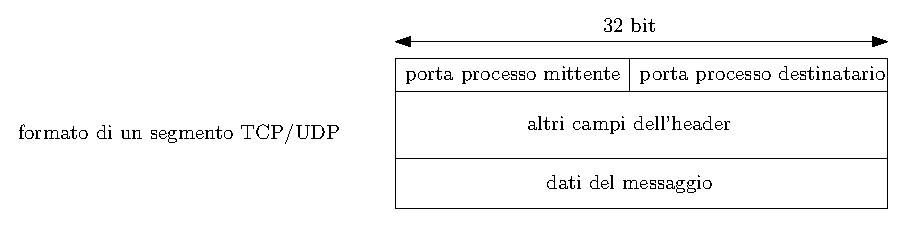
\includegraphics[width=0.9\textwidth ]{images/segmento.eps}
\end{center}
\subsubsection{Demultiplexing UDP e TCP}
Vediamo adesso come funziona il demultiplexing per i due differenti protocolli di trasporto, partendo con
UDP.\acc
Quando si crea un socket (canale virtuale), si deve specificare la porta locale del proprio host:\acc
\code{DatagramSocket mySocket1 = new DatagramSocket(12534);}
\acc
Per inviare un datagramma al socket UDP, bisogna specificare l'indirizzo IP di destinazione, e la porta del
processo di destinazione. Tramite l'IP, verrà individuato sulla rete l'host di destinazione, esso riceverà un
segmento UDP, verrà letto nell'header il campo relativo alla porta di destinazione, ed indirizzerà il
segmento al socket relativo a quel numero di porta.\acc
Per eseguire il demultiplexing nel destinatario, verrà utilizzato esclusivamente il numero di porta
del processo destinatario, il trasferimento UDP ha lo scopo di inviare un messaggio, e non di stabilire una
connessione, se arrivano ad un host due differenti datagrammi IP/UDP con la stessa porta di destinazione ma
diversi IP di origine (due diversi mittenti comunicano con lo stesso processo destinatario), semplicemente
entrambi i messaggi verranno indirizzati allo stesso socket ricevente.\acc
Nel caso del TCP, è differente, tale protocollo ha lo scopo di aprire una connessione persistente fra due
processi, ogni processo destinatario, non avrà un singolo socket che riceve tutti i segmenti, ma avrà
un socket per ogni connessione, quindi per ogni mittente.\acc
Un segmento IP/TCP quindi avrà bisogno di essere indirizzato nel socket corretto, non sarà più necessario
il numero di porta e l'IP del destinatario, ma per eseguire il demultiplexing, sarà anche necessario
distinguere i differenti host mittenti. \acc
Ogni socket sarà quindi identificato da una tupla composta da 4 valori:\begin{itemize}
    \item IP di origine
    \item Numero di porta di origine
    \item IP di destinazione
    \item Numero di porta di destinazione
\end{itemize}
Il multiplexing/demultiplexing non avviene però esclusivamente al livello di trasporto, ma anche su altri
livelli (verrà visto in seguito).
\subsection{UDP}
UDP è l'acronimo di \textit{User Datagram Protocol}, perché viene utilizzato il termine datagramma se si
parla di un segmento al livello di trasporto? Tale protocollo fornisce il servizio di trasporto senza
stabilire una connessione, è un sistema best-effort privo del concetto di handshake, si usa la parola datagramma
perché il segmento UDP è molto semplice, non c'è molta aggiunta di informazioni, l'header è molto piccolo.
\acc
Non c'è alcun controllo della congestione, un segmento UDP verrà inviato a prescindere dal traffico sulla
rete, viene utilizzato sulle applicazioni multimediali (streaming), dal DNS e da HTTP/3, che
gestisce il trasferimento affidabile a livello applicativo. \acc
Tale protocollo è estremamente semplice, non fa altro che ricevere un messaggio dall'applicazione, aggiungere
un header UDP, ed inviarlo al livello di rete, un segmento UDP ha il seguente formato:\begin{center}
    \includegraphics[width=0.9\textwidth ]{images/segmentoUDP.eps}
\end{center}
Il campo \textbf{checksum}, è un valore intero che serve a rilevare eventuali errori nel messaggio, quali
la modifica di alcuni bit dovuta ad interferenze elettromagnetiche. Quando viene composto un
segmento UDP, esso viene suddiviso in pezzi da 16 bit, che verranno trattati come un numero
intero in complemento ad 1, per poi essere sommati, dando quindi un valore che sarà appunto
il checksum.\acc
Il destinatario, si occuperà di eseguire lo stesso procedimento, ottenendo una somma, se essa differisce
dal campo checksum, vuol dire che c'è stato un errore ed alcuni bit sono cambiati, sarà poi compito
del destinatario decidere se scartare il segmento. Il checksum si imposta a zero nel caso non
si voglia utilizzare, esso è utilizzato su più livelli e non solo nei segmenti al livello di trasporto.
\subsection{Principi di Trasferimento Affidabile}
I protocolli al livello di trasporto non si occupano solo di creare
una comunicazione virtuale fra due processi su host diversi, ma anche di
garantire una comunicazione affidabile. Abbiamo visto come uno dei due
principali protocolli, l'UDP, non garantisce nulla di tutto ciò, in questo
capitolo si presenteranno dei concetti fondamentali, che saranno poi ripresi
dal TCP.\acc
Supponiamo di voler comunicare attraverso un canale in maniera
monodirezionale, ossia inviando dati esclusivamente da un host
all'altro. Per una comunicazione di questo tipo, è comunque necessario
un canale \textit{bidirezionale}, dato che l'host ricevente,
deve poter notificare al mittente di aver ricevuto correttamente il
messaggio.\acc
Ci occuperemo quindi di costruire un protocollo su un canale bidirezionale
\textit{inaffidabile}, la complessità del lavoro che dovrà impiegare tale
protocollo dipenderà dall'inaffibadilità del canale. Un altro problema
dipende dal fatto che il mittente ed il destinatario non conoscono
lo stato l'uno dell'altro.\acc
Costruiremo un astrazione di un protocollo chiamato
\textbf{rdt}, i dati viaggiano su un singolo canale, le informazioni di
controllo su entrambi i canali. Per descrivere il funzionamento del protocollo
useremo le \textbf{FSM}, ossia le macchine a stati finiti.
\subsubsection{rdt 1.0}
Costruiamo un'astrazione di un protocollo partendo da alcune assunzioni riguardanti possibili
inaffidabilità della comunicazione, aggiungendone sempre di più,
avvicinandoci ad un caso reale. Il protocollo rdt 1.0 si baserà su un
canale di comunicazione affidabile, in cui non ci sono perdite di
pacchetti o errori sui bit.\acc
Semplicemente, il mittente che riceve un messaggio dal livello applicativo,
lo incapsulerà in un pacchetto, per poi inviarlo ai livelli inferiori.
Il destinatario riceverà il pacchetto dai livelli inferiori,
effettuerà il decapsulamento ed invierà il messaggio al giusto
processo tramite il numero di porta.\begin{center}
    \includegraphics[width=\textwidth ]{images/rdt1.0.eps}
\end{center}
Risulta molto semplice tale implementazione data l'assunzione di un
canale totalmente affidabile.\acc
\textbf{Appunto sulla notazione} : \begin{itemize}
    \item rdt\_send(data) - il protocollo invia il messaggio al
          destinatario.
    \item packet = make\_packet(data) - il messaggio da inviare viene
          incapsulato in un pacchetto.
    \item udt\_send(data) - il pacchetto incapsulato viene inviato
          al socket tramite un protocollo inaffidabile.
    \item rdt\_receive(packet) - il protocollo riceve il pacchetto dal mittente.
    \item extract(packet,data) - il protocollo si occupa di eseguire il decapsulamento del pacchetto,
          data conterrà il messaggio estratto.
    \item deliver\_data(data) - il messaggio estratto viene inviato all'applicazione.
\end{itemize}
\subsubsection{rdt 2.0}
Consideriamo adesso un canale che non è al 100\% affidabile, ossia che, con una certa probabilità,
causi degli \textit{errori} sui bit, che dovranno essere rilevati tramite il campo checksum\footnote{
    si assume che il checksum sia infallibile e rilevi sempre errori, se presenti
} nell'header.
Sono necessari i seguenti costrutti:
\begin{itemize}
    \item Con il termine \textbf{ACK}, si intende un pacchetto che il destinatario invia al mittente in seguito
          alla ricezione di un messaggio, ed ha lo
          scopo di notificare a quest'ultimo che tale messaggio non presenta errori nei bit.
    \item Con il termine \textbf{NAK}, si intende un pacchetto che il destinatario invia al mittente in seguito
          alla ricezione di un messaggio, ed ha lo
          scopo di notificare a quest'ultimo che tale messaggio presenta errori nei bit, appositamente rilevati
          tramite il checksum.
\end{itemize}
Se il destinatario dovesse notificare un NAK, sarà necessario re-inviare il pacchetto che è stato modificato.
Per ragioni di semplicità, tale protocollo utilizzerà una politica di invio pacchetti \textbf{stop-and-wait},
consiste nell'inviare un singolo pacchetto alla volta, ed inviare il pacchetto successivo solo quando
si ha la certezza che quello precedente sia stato consegnato.\begin{center}
    \includegraphics[width=1\textwidth ]{images/rdt2.0.eps}
\end{center}
Il protocollo è ancora relativamente semplice, il mittente dopo aver inviato il pacchetto, attende di ricevere un
ACK oppure un NAK, nel primo caso, passerà al prossimo pacchetto, altrimenti, si occuperà di re-inviare il pacchetto
corrotto. Il destinatario invece, si occuperà semplicemente di ricevere pacchetti, controllare se sono corrotti tramite
l'operazione \code{is\_corrupt(packet)}, ed inviare un eventuale ACK o NAK al destinatario.
C'è però un assunzione in questo modello che non è stata considerata.
\subsubsection{rdt 2.1}
L'rdt 2.1 si occupa di gestire anche un possibile errore sui bit dei pacchetti ACK/NAK, un pacchetto corrotto di questo
tipo non può essere interpretato dal mittente, quindi come soluzione, quest'ultimo ri-invierà il pacchetto, se il messaggio
corrotto però in origine era un ACK, si avrà un pacchetto duplicato che il destinatario dovrà scartare.\acc
Ad ogni pacchetto verrà aggiunto un numero di controllo, che identificherà il numero di sequenza del pacchetto, al
destinatario sarà necessario leggerlo per controllare se tale pacchetto è nuovo oppure è una ritrasmissione
del pacchetto precedente, scaturita da un ACK/NAK corrotto. Tale numero di sequenza sarà implementato con un singolo
bit, che può essere 0 oppure 1, nel modello stop-and-wait sono necessari solo questi due valori.\begin{center}
    \includegraphics[width=0.9\textwidth ]{images/rdt2.1.eps}
\end{center}
Il mittente manda il pacchetto 0, se riceve un ACK/NAK corrotto, lo ri-invierà, se il destinatario si aspettava un pacchetto
1, in quanto aveva ricevuto correttamente il pacchetto 0, scarterà il pacchetto.
\subsubsection{rdt 3.0}
Il problema principale che non è ancora stato considerato riguarda l'eventualità che un pacchetto venga
\textit{perso}, ebbene è un evento molto comune nelle reti, e se si vuole garantire un trasferimento affidabile,
si deve considerare un modo per evitare tale perdita, mantenendo l'integrità dei dati.\acc
Supponiamo nell'rdt 3.0, che il canale possa causare una perdita di pacchetto, il mittente dovrà accertarsi che ogni pacchetto
inviato sia ricevuto, il destinatario non è al corrente dello stato del mittente, quindi esso potrebbe essere totalmente
ignaro che un pacchetto a lui destinato è stato perso.\acc
Il mittente, sa che un pacchetto è stato perso se non riceverà alcun ACK (o NAK) da parte del destinatario, per ogni pacchetto
inviato sarà quindi previsto un \textit{timer}, se entro un lasso di tempo stabilito, il mittente non riceverà alcun messaggio
di ACK, il pacchetto sarà considerato perso, e sarà inviato nuovamente.\begin{center}
    \includegraphics[width=1\textwidth ]{images/rdt3.0.eps}
\end{center}
Se viene ricevuto un pacchetto ACK con un numero non atteso, non viene fatto nulla, in quanto scatterà ugualmente
il timeout, non vengono più usati pacchetti ACK e NAK, ma esclusivamente pacchetti ACK.
\subsubsection{Pipelining}
Il problema è che tale protocollo convive con le restrizioni di un paradigma stop-and-wait, e l'attesa di un round trip
time per ogni pacchetto prima di poter inviare il prossimo riduce drasticamente le prestazioni, bisogna utilizzare un modello
di \textit{pipelining}, ossia includere la possibilità per il mittente, che esso possa inviare pacchetti senza dover
attendere che quelli precedenti siano stati correttamente consegnati. Vediamo i due paradigmi di pipelining principali.\acc
Il modello \textbf{go-back-n} permette al mittente di trasmettere più pacchetti contemporaneamente, può inviare al destinatario
al più $n$ pacchetti senza riceverne i rispettivi ACK. Alla ricezione di ogni pacchetto, il destinatario invierà un
ACK \textbf{comulativo}, i pacchetti sono numerati ed ordinati in sequenza, ed un ACK di numero $x$ indica che sono
stati ricevuti tutti i pacchetti sino al pacchetto $x$, e se ne necessitano dall'$x+1$-esimo in poi.\acc
Il timer, farà riferimento al pacchetto più "vecchio" inviato del quale non è stato ricevuto l'ACK, se scade,
verranno re-inviati tutti gli $n$ pacchetti da quest'ultimo in poi. I pacchetti che sono stati ricevuti ma in un ordine
sbagliato (ad esempio, si è in attesa del pacchetto 3 ma viene consegnato il pacchetto 4) verranno scartati, oppure
memorizzati in un buffer.\begin{center}
    \includegraphics[width=1\textwidth ]{images/go-back-n.eps}
\end{center}
L'altro costrutto di pipelining è noto con il nome di \textbf{selective repeat}, piuttosto che inviare un ACK
comulativo, ne viene inviato uno \textbf{selettivo}, riservato ad ogni singolo pacchetto, i pacchetti arrivati
in un ordine sbagliato, verranno salvati in un buffer, in questo modo, il mittente avrà una finestra di $n$ pacchetti
da poter inviare, ed il destinatario avrà una finestra di $n$ pacchetti da poter mantenere nel buffer, inoltre ogni
pacchetto ha il suo personale timer.\acc
Tale metodo risulta efficiente in quanto non è necessario dover inviare nuovamente l'intera finestra di $n$ pacchetti,
e riduce il grado di ridondanza, inoltre se la rete è congestionata, la rispedizione di tutti i pacchetti
peggiora la congestione. \acc
Il destinatario salverà i pacchetti nel buffer, quando avrà a disposizione la giusta sequenza ordinata, li invierà
al livello applicativo, decapsulandoli.\begin{center}
    \includegraphics[width=1\textwidth ]{images/selectiveRepeat.eps}
\end{center}
Anche se tale astrazione è stata costruita per una comunicazione mono-direzionale, nulla vita ad un pacchetto che
trasporta i dati, di trasportare anche i riscontri ACK, tale tecnica è nota con il nome di \textit{piggy-backing},
permettendo a due enti di comunicare e contemporaneamente notificarsi dell'ascolto.\acc
Un problema noto del selective repeat risiede nelle dimensioni della finestra del ricevitore, la mancata sincronizzazione
fra la finestra del mittente e quest'ultima causa gravi conseguenze quando si ha a che fare con un intervallo finito
di numeri di sequenza, si osservi il seguente esempio, in cui il range di numeri di sequenza per i
pacchetti sono [0,1,2,3] e la finestra del ricevitore ha ampiezza 3:\begin{center}
    \includegraphics[width=\textwidth ]{images/ErroreSelectiveRepeat.eps}
\end{center}
Il primo pacchetto ed il quinto pacchetto, hanno entrambi numero di sequenza 0. Il mittente, riceve correttamente
i primi tre pacchetti, con numeri di sequenza 0, 1 e 2, e la sua finestra verrà spostata sui pacchetti
3, 0 ed 1, che sono rispettivamente il quarto, il quinto ed il sesto.\acc
Il fatto è che, a seguito della perdita dei pacchetti ACK, il mittente non sa che i primi tre pacchetti sono stati
ricevuti, ri-invierà quindi il primo pacchetto con numero di sequenza 0 a seguito del timeout. Qui, il destinatario,
sta attendendo il quinto pacchetto che ha numero di sequenza 0, e riceve il primo pacchetto, anche esso con numero di
sequenza 0.\acc
Il destinatario interpreterà il primo pacchetto come se fosse il quinto, essendo che essi hanno lo stesso numero di
sequenza, tale errore causa una grave corruzione dei dati ricevuti.\acc
Per evitare ciò, è necessario sincronizzare l'ampiezza della finestra del destinatario, con la sequenza dei
numeri dei pacchetti, secondo tale relazione: \begin{itemize}
    \item Se i numeri di sequenza sono $2^m$ (Ad esempio, [0,1,2,3] sono $2^2$).
    \item La finestra del ricevitore deve essere grande $2^{m-1}$ (Ad esempio : $2^{2-1}=2^1=2$).
\end{itemize}
\subsection{TCP - parte 1 : Affidabilità e Connessione}
\subsubsection{Struttura del Segmento}
Il protocollo TCP vede il trasferimento dei dati, non come l'invio di segmenti, ma come l'invio di un
flusso di byte che compongono i messaggi, tale flusso deve arrivare dal mittente al destinatario in un
preciso ordine, è un protocollo bidirezionale che prevede una misura massima per la dimensione dei segmenti,
detta $MSS$ (solitamente 1460 byte).\acc
Il TCP permette ai due enti che comunicano di stabilire una connessione virtuale, di cui il resto della rete
non è a conoscenza. Utilizza dei riscontri ACK comulativi, e sfrutta il pipelining per l'invio di più
pacchetti. Con il termine \textbf{handshake}, si intende l'azione in cui i due enti stabiliscono la
connessione, tramite dei messaggi di controllo. Un segmento TCP è lo stesso sia per un messaggio di invio dati, sia
che per un messaggio di ACK (dato che utilizza il piggy-backing), ed è il seguente:\begin{center}
    \includegraphics[width=0.5\textwidth ]{images/TCPsegment.eps}
\end{center}
Il numero di sequenza non si riferisce al numero d'ordine del segmento, ma si riferisce al numero d'ordine
del primo byte del segmento di cui fa riferimento.\begin{quote}\color{gray}
    Ad esempio, si vuole mandare un messaggio di 10 byte, verrà incapsulato in 2 segmenti TCP di
    5 byte ciascuno, il primo segmento conterrà i byte dal numero 1 al numero 5, avrà quindi numero di
    sequenza 1, il secondo segmento conterrà i byte dal numero 6 al numero 10, avrà quindi numero di
    sequenza 6.\color{black}
\end{quote}
Il numero dell'ACK fa riferimento al byte successivo atteso, un numero di ACK $x$ indica che sono stati ricevuti tutti
i byte dal primo fino al $x-1$ esimo (l'ACK è comulativo). Il campo \textit{"INFO"} contiene delle informazioni come il numero di lunghezza
dell'header, un flag che indica se il checksum è in utilizzo oppure no, dei flag riguardo la gestione/sincronizzazione
della connessione ed altre informazioni.\acc
Il campo \textit{"finestra del ricevitore"} indica il numero di byte che il destinatario può "accogliere",
è necessario per il controllo del flusso, se il destinatario è "ingolfato", tale numero
di byte sarà più basso, imponendo al mittente di porre limite al numero di pacchetti che può inviare, per non intasare
ulteriormente la connessione. Il campo \textit{"opzioni aggiuntive"} contiene informazioni come la lunghezza
del messaggio.\acc
La gestione dei segmenti arrivati fuori ordine, non è considerata dal TCP, bensì dipende dall'implementazione.
\subsubsection{Gestione del Timer}
Abbiamo visto che un protocollo che ha lo scopo di garantire un trasferimento affidabile deve servirsi di un timeout
per la ritrasmissione dei pacchetti andati perduti, ma come va dosato il tempo effettivo di durata del timer?\acc
È chiaro che, il timeout deve essere almeno uguale o superiore al RTT (\textit{round trip time}), altrimenti ogni pacchetto
inviato scadrebbe in un timeout, il punto è che il RTT è variabile, e deve essere misurato da un timer, chiameremo
il tempo di RTT effettivo misurato dal timer $sampleRTT$, tramite tale misurazione per un pacchetto,
vogliamo stimare il RTT del pacchetto successivo, mantenendo la stima regolare, senza che sia troppo condizionata dalle
oscillazioni (variabilità) del $sampleRTT$.\acc
Viene utilizzata una tecnica nota come \textbf{EWMA} (exponential waited moving avarage), che tramite l'uso di un
peso $\alpha$ (numero reale fra 0 ed 1), utilizza le misurazioni precedenti per stimare il RTT successivo. Si indica con
$RTTstimato(t)$, la stima del RTT al tempo $t$, si ha che:
$$ RTTstimato(t) = (1-\alpha)\cdot RTTstimato(t-1)+\alpha \cdot SampleRTT$$
Se $\alpha = \nicefrac{1}{2}$, il RTT stimato sarà una media fra il RTT precedentemente stimato e quello
precedentemente misurato. Un valore tipico che si utilizza è $\alpha=0.125$.\acc
Il time out necessita inoltre di un minimo spazio, margine di sicurezza, in modo da essere di poco superiore
al RTT stimato, il valore effettivo che verrà utilizzato per il timeout, sarà pesato da tale margine di sicurezza
noto come $DevRTT$, misura la precisione della stima, ed è influenzato dalla variabilità del $SampleRTT$.
$$ DevRTT(t) = (1-\beta)\cdot DevRTT(t-1) + \beta\cdot(|SampleRTT-RTTstimato(t-1)|) $$
Dove $\beta$ è un numero reale fra 0 ed 1, viene utilizzato come peso, il valore
$|SampleRTT-RTTstimato(t-1)|$ non è altro che la differenza fra il RTT stimato ed il
RTT effettivo. Il tempo effettivo del timeout sarà:
$$ timeout=RTTstimato+4\cdot DevRTT$$
Si osservi il seguente grafico che mostra la differenza fra il RTT misurato ed il RTT stimato (quest'ultimo risulta
regolare e meno soggetto ad oscillazioni).\begin{center}
    \includegraphics[width=\textwidth ]{images/RTTstimato.eps}
\end{center}
\subsubsection{Semplificazione del TCP, Gestione del Flusso e della Connessione}
Vediamo adesso il funzionamento del TCP in maniera approssimativa, cominciando dal ruolo del \textbf{mittente},
esso riceve un messaggio dal livello applicativo, tale messaggio viene incapsulato in un segmento TCP con
l'aggiunta di un header, dopo di che, se non vi è già un timer in esecuzione, viene avviato (si ricordi che
è in esecuzione un solo timer valido per il segmento inviato meno recentemente per la quale non si è ricevuto
ancora l'ACK).\acc
All'avvenimento di un timeout, il mittente dovrà ri-inviare il segmento in questione, riavviando anche il timer.
Alla ricezione di un ACK (che si ricorda essere comulativo), viene aggiornata la finestra di pacchetti
da inviare, se vi sono ancora pacchetti il cui invio non è confermato, partirà un timer associato al pacchetto
inviato meno recentemente fra questi ultimi.\acc Vediamo il comportamento del \textbf{destinatario}:\begin{itemize}
    \item \textbf{evento} : arrivo di un segmento in ordine,
          con numero di segmento atteso,
          ossia per cui tutti i segmenti precedenti  ad esso sono
          già stati confermati  (situazione regolare) \\ \textbf{risposta} : si attende un tempo (solitamente 500ms) prima
          di inviare l'ACK, questo delay serve a coprire
          situazioni in cui, dovesse arrivare un nuovo segmento (successivo a
          quello originale)  pochi istanti dopo (riducendo il numero di ACK
          complessivi inviati).
    \item \textbf{evento} :arrivo di un segmento in ordine, con numero
          di segmento atteso,  ma un segmento precedente ricevuto,
          non è ancora stato confermato
          tramite l'invio di un ACK (complementare
          all'evento precedente)\\
          \textbf{risposta} : si invia immediatamente un ACK comulativo,
          confermando entrambi i segmenti.
    \item \textbf{evento} : arrivo di un segmento fuori ordine\\
          \textbf{risposta} : si invia immediatamente un ACK duplicato in
          cui si richiede il segmento atteso in ordine
    \item \textbf{evento} : arrivo di un segmento che riempie
          parzialmente o completamente un gap\\
          \textbf{risposta} : si invia immediatamente un ACK
\end{itemize}
Nell'ultimo caso, in cui si parla di "gap" da riempire, si intende una situazione in cui il destinatario ha confermato
(ad esempio), i segmenti 1,2 e 3, è in attesa del 4, ma mantiene nel buffer i segmenti 5 e 6, l'arrivo del
segmento 4, farà si che verranno mandati al livello applicativo i segmenti 4,5 e 6, facendo si che il destinatario
invia un ACK comulativo con numero 7 (si ricordi che il numero di segmento si riferisce ai byte e non al segmento
stesso, sono stati utilizzati numeri sequenziali per semplicità, nell'assunzione che ogni segmento abbia 1 byte).\acc
Si osservi la seguente situazione:\begin{center}
    \includegraphics[width=\textwidth ]{images/fastRetrasmit.eps}
\end{center}
Introduciamo il \textbf{controllo del flusso}, si consideri uno scenario, dalla parte di un destinatario
TCP, in cui il livello di rete fornisce segmenti più rapidamente rispetto a quanto il livello di applicazione
possa leggerne, riempendo il buffer del socket TCP. \acc In tal caso il destinatario, dovrà notificare il mittente del
fatto che esso sta trasmettendo troppo \textit{rapidamente}, almeno più di quanto esso possa processare i
segmenti. Il destinatario avviserà il mittente tramite gli appositi campi nell'header relativi alla sua finestra
di ricezione.\acc
Si osservi come questa è una congestione \textit{locale}, e non da parte della rete, può avvenire anche se la rete
è totalmente libera, e dipende eslcusivamente dalla velocità di elaborazione dei segmenti del destinatario.\acc
Il destinatario TCP "dichiara" lo spazio che ha libero per i segmenti nel buffer tramite il
campo \code{rwnd} nell'header, ed il mittente imposta la sua finestra di segmenti possibilmente
inviabili prima di essere confermati, proprio al valore di \code{rwnd}, ciò garantisce l'assenza di
sovraccaricamento nel buffer del ricevitore.\acc
Il TCP si occupa anche di creare una \textbf{connessione} stabile fra i due comunicatori, tramite la già
citata operazione di \textbf{handshake} (stretta di mano). Consiste, nella dichiarazione da parte dei due comunicatori
di voler aprire una connessione (richiesta ed accettazione), e nel concordamento di alcuni parametri, quali il
numero di porta, la finestra di ricezione, oppure il numero iniziale di segmento atteso.\acc
Inizialmente il TCP si serviva di un handshake \textit{a 2 vie}:\begin{enumerate}
    \item
          colui che voleva aprire la connessione (richiedente)
          inviava una richiesta di connessione ad un host (richiesto), tale richiesta era accompagnata da un numero
          $x$.     \item  il richiesto, rispondeva con un messaggio di "accettazione", re-inviando il numero $x$ per indicare
          che la risposta è relativa alla richiesta dello stesso numero.
    \item a quel punto, il richiedente era pronto ad inviare dati, inviando però, anche un valore numerico aggiuntivo,
          ossia $x+1$.
    \item il richiesto, riceve i dati, ed invia un messaggio di ACK, con numero di sequenza $x+1$, alla ricezione di quest'ultimo
          la connessione sarà ufficialmente stabilita.
\end{enumerate}
In alcuni scenari, l'handshake a 2 vie può risultare problematico, ad esempio quando il richiedente si disconnette
durante una richiesta di connessione, lasciando una connessione "aperta", per questo le implementazioni odierne del TCP
implementano l'handshake \textit{a 3 vie}:\begin{enumerate}
    \item il richiedente, sceglie un numero $x$, ed invia un messaggio TCP SYN.
    \item il richiesto che riceve il messaggio, sceglie un numero $y$, che sarà il primo numero di
          sequenza, ed invia al richiedente un ACK, con numero di sequenza richiesto $y$, insieme ad un valore aggiuntivo,
          ossia $x+1$.
    \item il richiedente riceverà il messaggio, verificando di aver ricevuto $x+1$, ciò indicherà che il
          richiesto è attivo, invierà poi un segmento (possibilmente
          già provvisto di dati), con numero di ACK $y+1$.
    \item il richiesto, una volta ricevuto il segmento con ACK $y+1$, avrà la certezza che il richiedente è attivo,
          e la connessione sarà ufficialmente stabilita.
\end{enumerate}
Tali numeri $x$ ed $y$ stabiliscono quindi il numero di sequenza iniziale, che molto spesso non è 0, infatti,
per ragioni di sicurezza,  tali due numeri sono selezionati casualmente.\acc
Quando una connessione deve essere \textit{chiusa}, colui che ha intenzione di interromperla invierà un segmento
con un flag \code{FIN=1}, colui che lo riceverà, risponderà con un ACK combinato con il proprio \code{FIN},
confermando la chiusura della connessione.
\subsection{TCP - parte 2 : Controllo della Congestione }
Quando i pacchetti arrivano ai router troppo rapidamente per essere gestiti dalla rete ed essere immediatamente
ritrasmessi, si crea un accodamento nei buffer dei router, essendo la memoria di questi buffer finita, all'aumentare
della coda alcuni pacchetti andranno scartati, causando una perdita di pacchetti.\acc
Supponiamo che, il mittente abbia perfetta conoscenza dei buffer dei router, sapendo se sono liberi o no,
facendo si che esso possa trasmettere solo quando possibile senza causare congestione. Supponiamo poi che il mittente
ritrasmetta eslcusivamente i pacchetti persi, sprecando in qualche modo il rate disponibile per questi ultimi.\acc
In uno scenario reale però, alcuni pacchetti possono essere ritrasmessi anche se non necessario, dato un prematuro scadere
del timer, quindi si aggiunge un ulteriore spreco della capacità. Durante uno scenario di congestione è necessario più
lavoro (ritrasmissioni) per un dato troughput, date le ritrasmissioni inevitabili.\begin{center}
    \includegraphics[width=\textwidth ]{images/perditaCongestione.eps}
\end{center}
Anche se la perdita sembra labile, il problema è che, queste ritrasmissioni in uno scenario con più
router/nodi sul percorso, causano una perdita do troughput \textit{catastrofica}, lo scarto di un pacchetto rende
sprecate le capacità ed il buffering di tutti i nodi utilizzati per quel pacchetto. I pacchetti tenderanno
ad avere una probabilità di passare per un nodo sempre più bassa, tendente a zero, così come il troughput.
\subsubsection{AIMD, Slow Start e Cubic}
Ciò fa capire che controllare la congestione è necessario. Vedremo un approccio end-to-end, in cui il mittente e destinatario
che comunicano "dedurranno" lo stato della congestione in base al ritardo e le perdite osservate.\acc
Il TCP di base, si occupa della congestione regolando la velocità di invio dei mittenti: Un mittente potrà
\textit{aumentare} (linearmente) la sua velocità di invio (aumentando il numero di segmenti della finestra) affinchè non si
causerà una perdita di pacchetti, a quel punto, ridurrà \textit{sostanzialmente} la velocità, venendo
dimezzata. Tale approccio è detto \textbf{AIMD} (Additive Increase Multiplicative Decrease):\begin{center}
    \includegraphics[width=0.8\textwidth ]{images/AIMD.eps}
\end{center}
Ogni RTT il rate di invio aumenta di 1 MSS (misura massima per la dimensione dei segmenti) fino a quando non viene
osservata una perdita. Se vengono ricevuti 3 ACK duplicati, il rate viene dimezzato, se invece avviene un
timeout il rate viene impostato ad 1 MSS.\acc Il fatto è che quando l'aumento lineare inizia da un valore
basso del rate, ci vorrà del tempo prima che esso raggiunga la soglia di perdita, ciò significa che, per un certo
lasso di tempo il mittente sta trasmettendo più lentamente di quello che effettivamente potrebbe, causando uno spreco
di banda, è possibile rendere questa crescita più veloce fino al raggiungimento del limite, per poi entrare
nella fase di AIMD. \acc Tale algoritmo è noto come \textbf{slow start}, consiste nel far incrementare la finestra di
invio in maniera esponenziale, si aumenta di 1 MSS per ogni ACK ricevuto:\begin{itemize}
    \item All'inizio si invia un segmento.
    \item Dopo un RTT si riceve un ACK e si inviano 2 segmenti.
    \item Dopo un RTT si ricevono 2 ACK e si inviano 4 segmenti.
    \item Dopo un RTT si ricevono 4 ACK e si inviano 8 segmenti.
    \item $\dots$
\end{itemize}\begin{center}
    \includegraphics[width=0.55\textwidth ]{images/slowStart.eps}
\end{center}
Quando è però che bisogna passare dalla crescita esponenziale (slow start) alla crescita
lineare (AIMD)? Quando la variabile \code{cwnd} = byte inviati al secondo raggiunge un valore
$x$ tale che $x = \dfrac{\code{cwnd'}}{2}$ dove \code{cwnd'} è il valore di \code{cwnd} prima dell'ultima perdita
di pacchetto. \acc
Si implementa una variabile \code{sstresh} che è impostata a $\dfrac{\code{cwnd'}}{2}$, quando il rate raggiunge
tale variabile, si passa allo stato di AIMD. A seguito di una perdita, il valore di \code{sstresh} si re-imposta
al nuovo valore di $\dfrac{\code{cwnd'}}{2}$ dato dalla nuova perdita. Questo comportamento è adottato dalla versione
del TCP nota come \textit{Tahoe}, la versione TCP \textit{Reno} passa direttamente allo stato di
AIMD dopo l'arrivo di 3 ACK duplicati. All'inizio della congestione, \code{sstresh} è impostato ad un valore di
default (nell'esempio seguente, è 12): \begin{center}
    \includegraphics[width=0.55\textwidth ]{images/sstresh.eps}
\end{center}
Esiste anche un approccio migliore per "sondare" la larghezza di banda utilizzabile, possiamo cambiare la pendenza
della crescita nella fase di "congestion avoidance", sia $W_{max}$ la velocità di invio quando è stata rilevata
la perdita per colpa della congestione.\acc Si suppone che lo stato della congestione nel frattempo non sia cambiato
in maniera significativa, quindi, piuttosto che crescere linearmente, il rate salirà
rapidamente verso $W_{max}$, e quando vi è in prossimità, ci si avvicinerà lentamente, sia $K$ l'istante di
tempo stimato in cui la dimensione della finestra raggiungerà $W_{max}$, aumenteremo tale finestra
in funzione del cubo fra la distanza tra il tempo corrente e $K$.\acc
Tale versione del TCP è detta \textbf{Cubic}, è la versione predefinita sulle distribuzioni di \textit{Linux} ed è
il TCP più popolare per i server web più diffusi.\acc
\begin{center}
    \includegraphics[width=0.55\textwidth ]{images/TCPcubic.eps}
\end{center}
Il comportamento del controllo della congestione può essere riassunto con la seguente FSM:
\begin{center}
    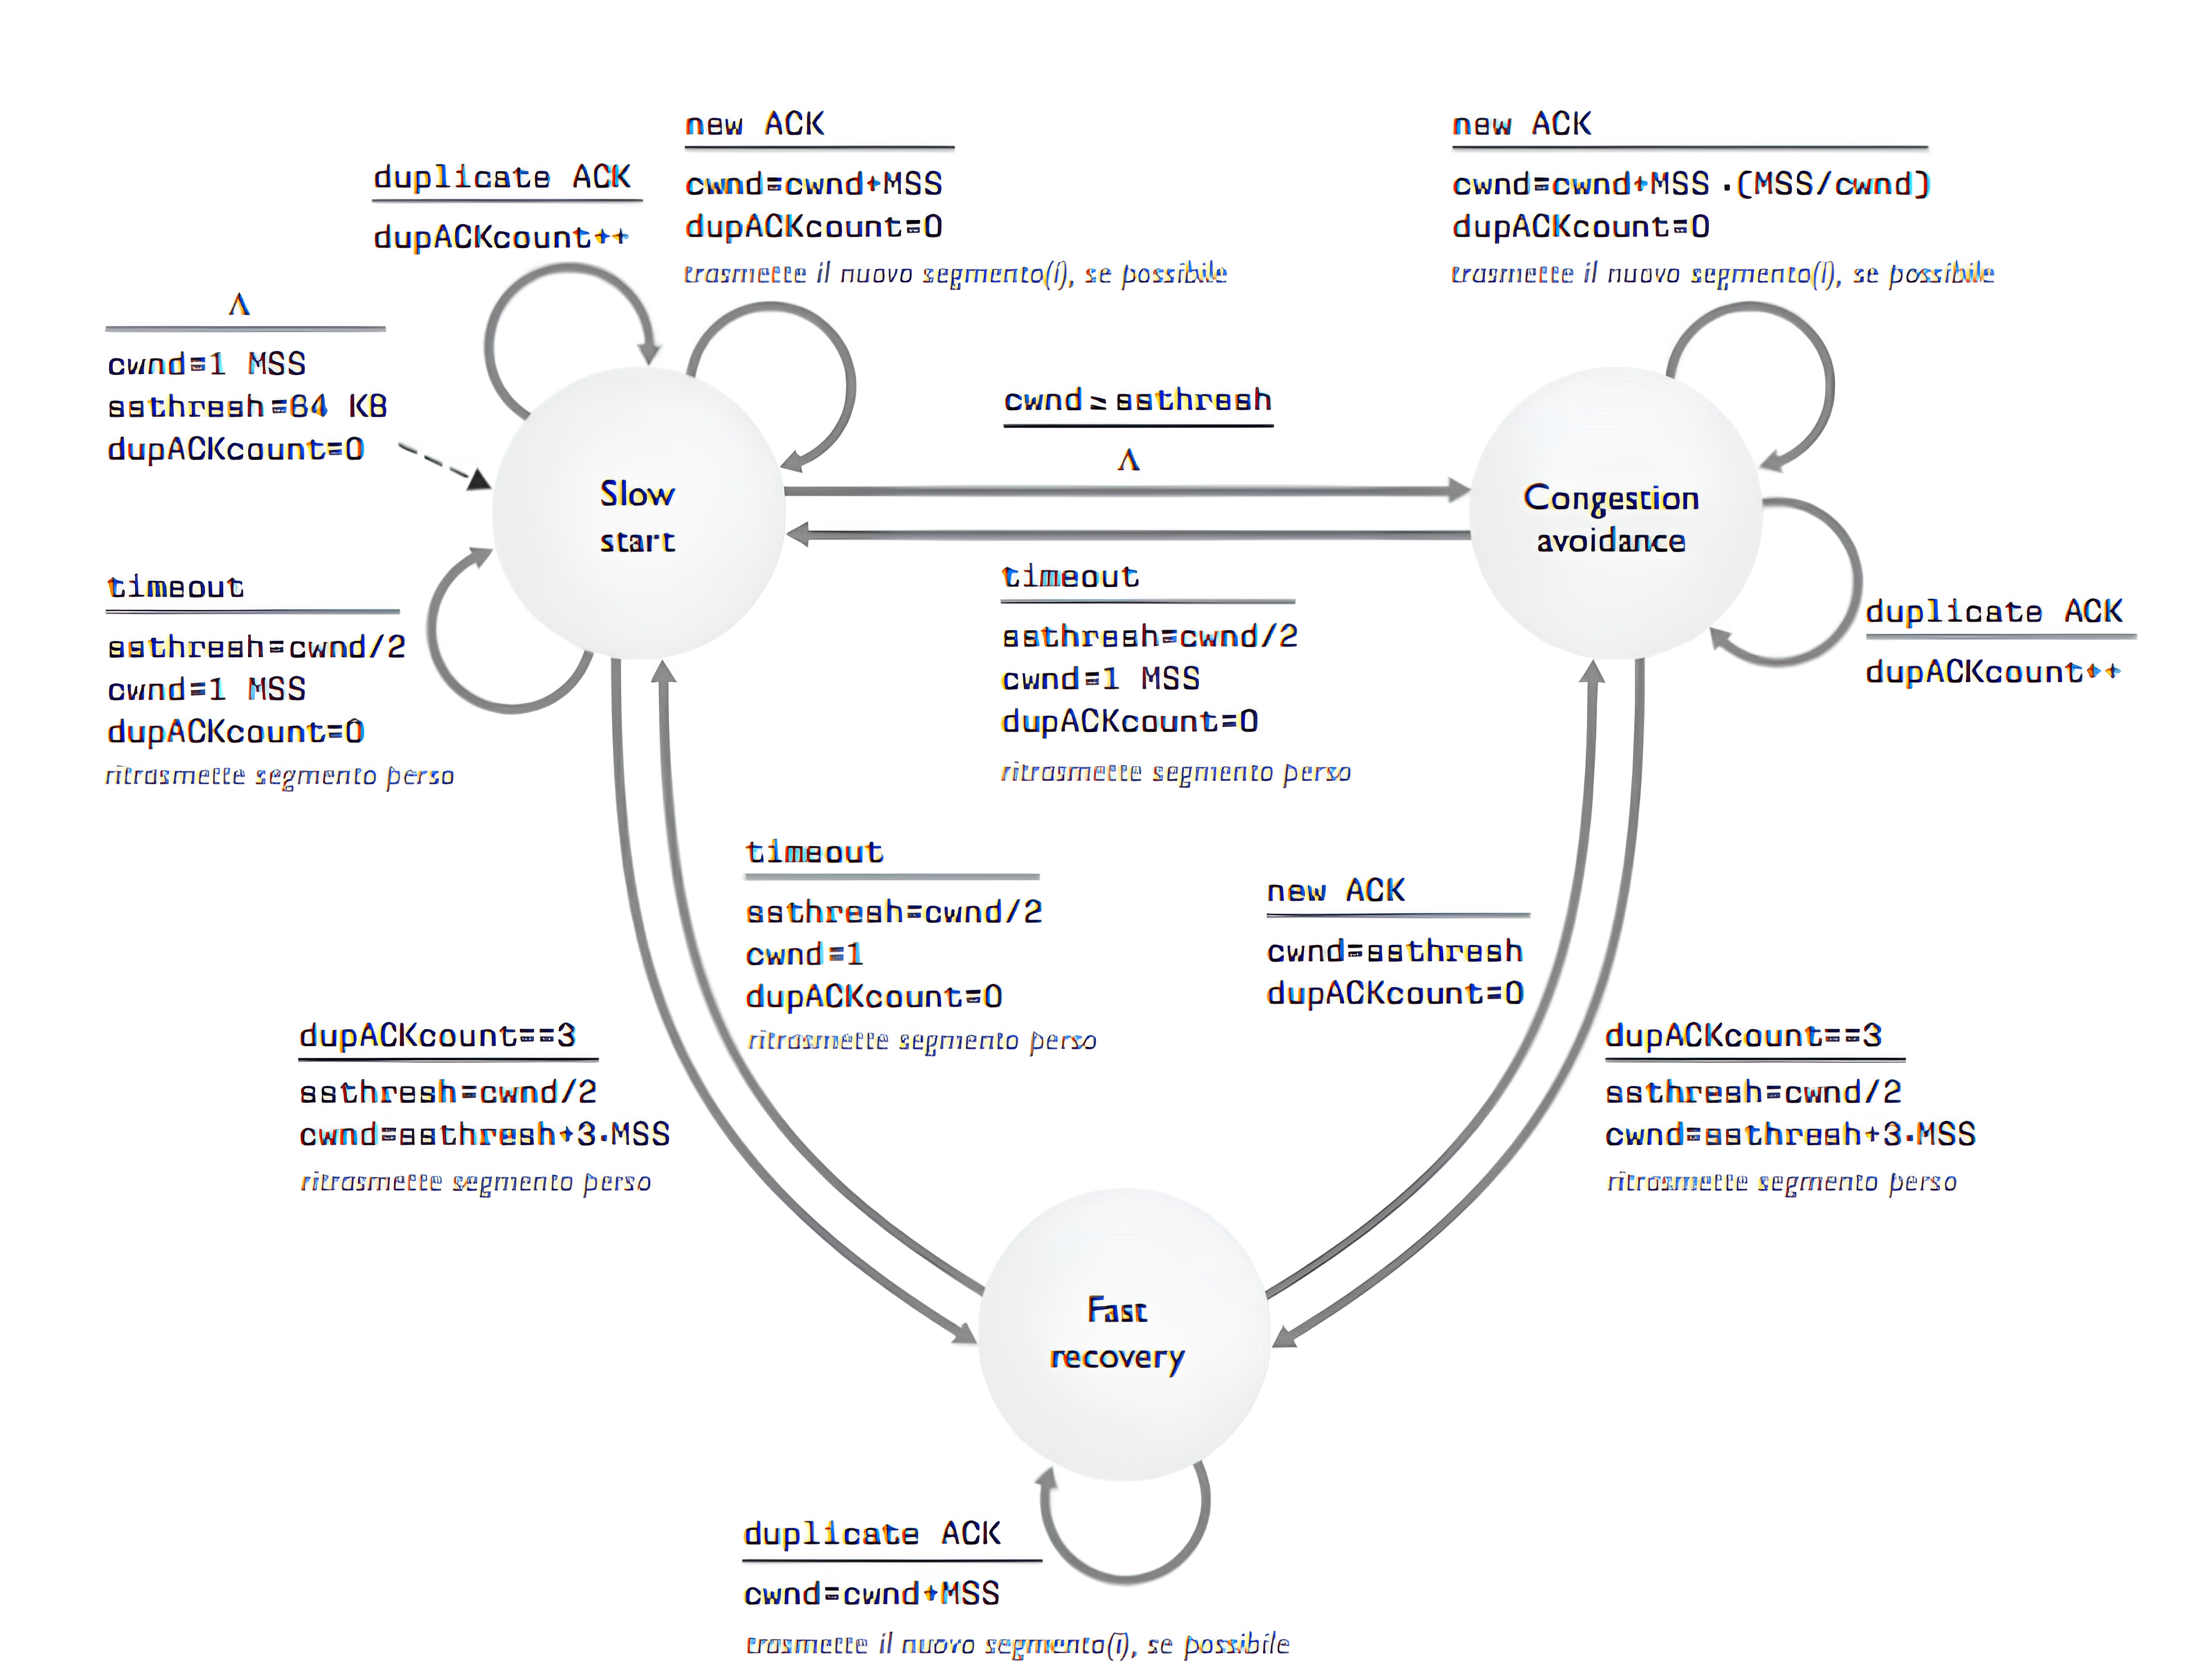
\includegraphics[width=0.8\textwidth ]{images/TCPfsm.png}
\end{center}
\subsubsection{Differenti Approcci TCP}
Il TCP è basato sull'aumento del rate di invio affinché non si registrano
perdite di pacchetti, dovute alla congestione di un link che funge
da collo di bottiglia. Esistono altri approcci basati su differenti
paradigmi : è possibile cercare di capire quando la coda in un router
si sta riempendo, in quanto a quel punto,
l'aumento del rate provoca anche un aumento del ritardo.\acc 
Viene misurato l'RTT tenendo conto del minimo osservato, ossia $RTT_{min}$, calcolando il troughput nella maniera 
seguente $$ \dfrac{BLS}{RTT_{min}}\;\;\;BLS = \text{ Byte inviati nell'ultimo stream }$$
Se il troughput è "vicino" al troughput "ottimale", ossia $\dfrac{\code{cwnd}}{RTT_{min}}$, allora  \code{cwnd} 
aumenta linearmente, altrimenti, se è "lontano", diminuisce linearmente.\acc 
Tale apporccio controlla la congestione senza indurre un aumento del troughput che cuserà una necessaria perdita, cerca 
di massimizzare il troughput cercando di mantenere il link "quasi pieno", funziona end-to-end e necessita di informazioni 
storiche sul percorso.\acc 
Un altro meccanismo può essere quello di inviare una \textbf{notifica esplicita (ECN)} di congestione, tramite 
due bit nell'intestazione IP che vengono contrassegnati dal router di rete per la quale passa il datagramma.\acc 
Il TCP si pone come obbiettivo quello di essere il più "equo" possibile, se $k$ connessioni TCP condividono 
un collegamento di bitrate $R$, ogni singola connessione dovrebbe avere a disposizione una velocità 
medi pari a $\nicefrac{R}{2}$, a prescendere dall'ordine in cui le connessioni vengono avviate.\acc 
Il problema è che un host può aprire più connessioni TCP, ottenendo quindi più velocità in quanto la velocità del 
collegamento è condivisa fra le singole connessioni TCP e non fra gli host che ne usufruiscono.\acc 
Molte applicazioni di rete al giorno d'oggi, non utilizzano TCP, bensì UDP, per poi gestire il controllo della 
congestione al livello applicativo, come HTTP/3 che utilizza il protocollo \textit{QUIC}, implementato in larga scala 
sui servizi di \textit{Google}.
\section{Livello di Rete - parte 1 : Il Piano dei Dati}
\subsection{Introduzione}
I protocolli che operano su tale livello, sono implementati su qualsiasi macchina che si può connettere 
ad una rete, e risultano complessi. Un pacchetto viene incapsulato in un datagramma IP per poi venire spedito 
nella rete, dove deve essere instradato fino al destinatario, a tal proposito, i router si occupano di 
leggere l'intestazione IP di un datagramma entrato in una porta in entrata, per poi smistarlo nelle porte di uscita.\acc 
La rete, basa il suo funzionamento su due costrutti principali:\begin{itemize}
    \item \textbf{forwarding} : Spostare i pacchetti che entrano dalla porta di ingresso di un router in 
    una delle sue porte di uscita, è un'operazione \textit{locale} che avviene su ogni router, i pacchetti vengono spostati 
    in base ai loro valori nell'intestazione, ed ogni router possiede delle tabelle associative che indicano dove 
    far uscire i datagrammi in base ai valori prima citati. 
    \item \textbf{routing} : Il processo per cui si determina \textit{globalmente} il percorso che un datagramma 
    deve seguire per arrivare dalla sorgente alla destinazione, tale processo avviene tramite dei dedicati 
    algoritmi di instradamento, con cui si riempioni i campi delle tabelle nei router sopra citate.
\end{itemize}
L'intero livello di rete si divide quindi in due parti, il \textbf{piano dei dati}, ossia l'insieme di costrutti e 
paradigmi relativi al forwarding, come il determinare come un datagramma in arrivo deve essere smistato, ed il 
\textbf{piano di controllo}, relativo al routing, ossia la determinazione di come il datagramma deve essere 
instradato sulla rete, tramite algoritmi di routing tradizionali (distribuiti ed implementati nei router), oppure 
implementati in server remoti, che hanno una visione globale dell'intera rete, e si occupano di aggiornare le
tabelle dei router.\acc Gli ISP spesso seguono questo tipo di approccio, avendo un server (o un insieme di server) centralizzati 
che si occupano di eseguire gli algoritmi, che risultano computazionalmente pesanti in quanto, il calcolo dell'instradamento 
nell'Internet moderno è molto complesso, data la presenza di milioni di router sparsi nel mondo.\begin{center}
    \includegraphics[width=1\textwidth ]{images/dataAndControlPlane.eps}
\end{center}
Il livello di rete non offre alcuna garanzia sulla consegna affidabile dei pacchetti, ne sui tempi di consegna, 
Internet è un servizio best-effort, implementato in maniera semplice, in modo da essere ampliato facilmente.
\subsection{Funzionamento del Router}
Il router è il device principale che opera sul livello di rete, e permette l'instradamento dei pacchetti, è disposto di una 
struttura detta \textbf{switching fabric}, implementata via hardware, in modo tale da permettere lo smistamento dei pacchetti in 
un lasso di tempo brevissimo, nell'ordine dei nanosecondi. È anche disposto di un classico processore per le operazioni 
del piano di controllo, anche se in tempi odierni la maggiorparte dei router delegano tale lavoro a dei server 
remoti (come precedentemente accennato). \acc 
Vi sono diverse terminazioni di linea, predisposte alla ricezione dei bit, una volta che il datagramma 
è entrato in una porta, agisce 
la switching fabric, che leggendo i valori nell'intestazione inoltra il datagramma in una porta di uscita, consultando 
la tabella di inoltro, tale operazione deve avvenire in un lasso di tempo brevissimo, più del rate di arrivo dei datagrammi, in modo 
da non causare bottleneck.\acc 
La tabella associa ad ogni indirizzo IP una porta di uscita, un indirizzo è composto da 32 bit, quindi la tabella teoricamente 
necessita di $2^{32} \simeq 4.3\cdot 10^9 $ entrate. Per evitare un numero così grande di entrate, è organizzata 
in maniera gerarchica, assegnando ogni porta ad un certo range di indirizzi.\begin{center}
    \begin{tabular}{|c|c|}
        \hline
        \rowcolor[HTML]{C0C0C0} 
        \textbf{range di indirizzi}            & \textbf{porta in uscita}        \\ \hline
        \rowcolor[HTML]{FFFFFF} 
        11001000  00010111  00010***  ******** & \cellcolor[HTML]{FFFFFF}porta 0 \\ \hline
        \rowcolor[HTML]{FFFFFF} 
        11001000  00010111  00010000  ******** & porta 1                         \\ \hline
        \rowcolor[HTML]{FFFFFF} 
        11001000  00010111  00011***  ******** & \cellcolor[HTML]{FFFFFF}porta 2 \\ \hline
        altrimenti                             & porta 3                         \\ \hline
        \end{tabular}
\end{center}
Alcuni bit meno significativi sono lasciati indefiniti, ed il range è rappresentato dai bit più significativi. Quando vi è 
un indirizzo in entrata, si esegue l'AND con gli indirizzi nella tabella (escludendo i bit indefiniti), e sarà scelta 
la porta dedicata all'indirizzo con cui avviene un match. \acc 
Cosa succede però nei casi in cui un indirizzo fa match con più di un indirizzo presente nella tabella?
\begin{center}
    \begin{tabular}{|c|c|}
        \hline
        \rowcolor[HTML]{C0C0C0} 
        \textbf{range di indirizzi}                                   & \textbf{porta in uscita}        \\ \hline
        \rowcolor[HTML]{FFFFFF} 
        {\color[HTML]{FE0000} 11001000  00010111  00010***  ********} & \cellcolor[HTML]{FFFFFF}porta 0 \\ \hline
        \rowcolor[HTML]{FFFFFF} 
        {\color[HTML]{FE0000} 11001000  00010111  00010000  ********} & porta 1                         \\ \hline
        \rowcolor[HTML]{FFFFFF} 
        {\color[HTML]{000000} 11001000  00010111  00011***  ********} & \cellcolor[HTML]{FFFFFF}porta 2 \\ \hline
        altrimenti                                                    & porta 3                         \\ \hline
        \end{tabular}\acc
        entrambi \color{red}MATCH \color{black}  con l'indirizzo 11001000  00010111  00010000 10110010
\end{center}
Viene selezionato l'indirizzo con il prefisso di bit definiti più lungo che è un match con l'indirizzo in entrata, nel 
caso sovrastante, il datagramma verrebbe inoltrato nella porta 1. \acc 
La switching fabric quindi si occupa di trasferire il datagramma nella porta di uscita, definiamo \textbf{switching rate} 
la velocità con la quale i pacchetti possono essere trasferiti dalle porta in ingresso a quelle in uscita. Se le porte in ingresso 
sono $n$ la velocità ideale di commutazione sarà $n\cdot $switching rate.\acc  
Nei router di prima generazione lo switching avveniva sotto il controllo di una vera CPU, il pacchetto veniva copiato nella 
RAM presente nel router e veniva poi processato, la velocità di lettura e scrittura della memoria limitava però lo 
switching rate.\begin{center}
    \includegraphics[width=0.7\textwidth ]{images/fabricMem.eps}
\end{center}
Successivamente si è optato per implementare via hardware dei bus appositi, più rapidi dei bus di sistema, ma sempre 
limitanti rispetto alle implementazioni moderne, che prevedono delle \textit{reti di interconnessione},
che sfruttano il parallelismo, frammentando il datagramma in celle di lunghezza fissa, facendolo commutare nella rete 
di interconnessione per poi ri-assemblarlo in uscita.\begin{center}
    \includegraphics[width=0.7\textwidth ]{images/fabricInterconnesso.eps}
\end{center}
I router moderni applicano lo "scaling", ossia implementano più piani di commutazione che operano in parallelo, permettendo 
un'aumento sostanziale dello switching rate, garantendo velocità elevate, ed una capacità di commutazione 
fino a 100 teraByte per secondo.\begin{center}
    \includegraphics[width=0.65\textwidth ]{images/fabricParallelo.eps}
\end{center}
\subsubsection{Accodamento}
L'accodamento interno al router (da non confondersi con l'accodamento visto nei capitoli precedenti) si verifica quando 
i pacchetti arrivanno nelle porte di input più rapidamente di quanto la switching fabric possa smistarli nelle 
porte di uscita. Se ciò avviene i datagrammi verrano accodati in un buffer di capienza limitata, quando raggiunge la dimensione 
massima sarà necessario eliminare dei pacchetti nel buffer secondo delle determinate politiche.\acc 
Il buffer deve avere una capienza che non sia ne limitata ne eccessiva, le dimensioni ottimali sono date dalla 
seguente formula empirica: $$\dfrac{ RTT\cdot c}{\sqrt{n}}$$
Dove $RTT$ è il round trip time tipico, $c$ è il bit rate ed $n$ è il numero di flussi presenti. Vediamo alcuni paradigmi di 
scheduling adottati nel selezionare un pacchetto da scartare quando il buffer è pieno.\begin{itemize}
    \item \textbf{FCFS} : I pacchetti vengono elaborati in ordine di arrivo, chi arriva prima ha la priorità, se il buffer 
    è pieno, i pacchetti nuovi verranno scartati. 
    \item \textbf{Prioritario} : I pacchetti verranno selezionati in base ad un grado di priorità dato dalle informazioni 
    presenti nell'header. Ad ogni grado di priorità viene assegnata una coda, ed i pacchetti delle code sottostanti verranno 
    considerati esclusivamente quando non vi saranno pacchetti in attesa nelle code sovrastanti.
    \item \textbf{Round Robin} : I pacchetti sono smistati in differenti code in base ad una classificazione che avviene 
    per via della loro intestazione, ciclicamente viene selezionata una nuova coda dalla quale si seleziona il pacchetto in 
    attesa, ogni classe quindi deve aspettare il proprio turno.
\end{itemize} 
Il Round Robin può essere generalizzato nella politica \textbf{Weighted fair queuing}, in cui ad ogni classe $i$ viene 
assegnato un peso $w_i$, e riceve una quantità di servizio (pacchetti selezionati per turno) pesata: 
$$ \dfrac{w_i}{\sum_{j=1}^nw_j}\;\;\;\;\;\;\;\;\;\;\;\;n=\text{ numero delle classi}$$
Il router deve anche occuparsi del cosiddetto \textbf{marking}: In situazioni in cui la rete è congestionata, vanno 
selezionati degli appositi pacchetti che verranno marcati come trasportatori dell'informazione riguardo la congestione.\acc 
Come accennato, alcuni router possono dare la precedenza ad alcuni pacchetti, oppure penalizzarli, in base alla loro intestazione, 
non sono strani casi in cui alcuni ISP hanno penalizzato pacchetti di competitor commerciali all'interno delle proprie reti 
private, è un problema di natura tecnica ma anche sociale ed economica. Diversi paesi hanno differenti approcci sulla neutralità 
della rete e sono necessari dei provvedimenti legali per stabilire regole e politiche di gestione.
\subsection{Il protocollo IP}
Tale protocollo, riguarda sia il formato del datagramma e la sua intestazione, sia le regole riguardanti la struttura 
degli indirizzi che identificano i terminali della rete. Un segmento TCP, UDP o di un qualsiasi altro protocollo di trasporto, 
viene incapsulato in un datagramma IP, che segue il formato seguente:\begin{center}
    \includegraphics[width=0.45\textwidth ]{images/ipDatagram.eps}
\end{center}
\begin{itemize}
    \item Il campo \textit{header len} identifica la lunghezza in byte dell'intestazione.
    \item Il campo \textit{ver} identifica la versione del protocollo IP 
    \item Il campo \textit{serv} specifica il tipo di servizio per la quale si sta utilizzando il datagramma, ad esempio, un ECN. 
    \item Il campo \textit{lunghezza} identifica la lunghezza in byte dell'intero datagramma, è variabile, può essere 
    al massimo di 65536 byte, ma un valore tipico è 1500 byte.
    \item I campi \textit{id 16 bit}, \textit{flags} e \textit{fragment offset}, sono necessari nei casi in cui 
    un segmento viene frammentato in più datagrammi. 
    \item Il campo \textit{TTL} è un numero intero positivo ed identifica il numero di hop/router intermedi per la quale può passare 
    il datagramma prima di essere scartato (l'utilizzo è stato accennato nel capitolo \ref{ritAccodamento}).
    \item Il campo \textit{upper layer} identifica che tipo di segmento di trasporto è stato incapsulato (ad esempio, se TCP o UDP).
    \item Il campo opzioni può contenere informazioni aggiuntive come il timestamp.
\end{itemize}
Il punto centrale dell'intestazione sono gli indirizzi IP di mittente e destinatario, l'indirizzo IP è un identificatore 
a 32 bit, ed identifica un \textit{interfaccia di rete} di un host o di un router, il primo ha solitamente due 
interfacce (Ethernet e wirless), mentre il secondo ne ha svariate. Per comodità, un IP viene letto 
in notazione decimale puntata a gruppi di 8 bit \begin{center}
    \begin{tabular}{cccc}
        \cellcolor[HTML]{FFFFFF}{\color[HTML]{000000} 11011111.} & 00000001. & 00000001. & \cellcolor[HTML]{FFFFFF}00000001 \\
        223.                                                     & 1.        & 1.        & 1                               
        \end{tabular}
\end{center}
Definiamo \textbf{sottorete}, un insieme di dispositivi connessi che possono comunicare (raggiungersi fisicamente) senza 
l'utilizzo di un router intermedio, i dispositivi di una sottorete condividono un range di bit più significativi nei 
loro indirizzi IP, che identifica la sottorete, quelli meno significativi identificano i singoli host.\begin{center}
    \includegraphics[width=1\textwidth ]{images/sottoreteIp.eps}
\end{center}
È possibile identificare un'intera sottorete tramite \textbf{subnet mask}, tramite la seguente notazione detta CIDR\begin{center}
    a.b.c.d/$x$ \\ 
    ad esempio : 200.23.16.0/23
\end{center}
Dove il numero $x$ seguito dallo slash rappresenta il numero di bit fissi dell'indirizzo, mentre $32-x$ rappresenta il 
numero di bit variabili, e conseguentemente l'insieme di indirizzi IP distinti che possono esistere in tale sottorette.
\begin{center}
    200.23.16.0/23 $\implies$ 11001000 00010111 0001000x xxxxxxxx
\end{center}
La sottorete nell'esempio sovrastante può identificare $2^4=16$ indirizzi IP differenti. La maschera viene spesso 
rappresentata come maschera binaria di 32 bit, dove vi è 1 nei bit fissi, e 0 nei bit variabili 
\begin{center}
    subnet mask 23 :\\ 11111111 11111111 11111110 00000000 = 255.255.254.0
\end{center}
Quando un host si connette ad una sottorete per la prima volta, che indirizzo IP gli viene assegnato? Ed in che modo 
può ricevere messaggi se non è identificabile? Esiste un protocollo apposito, implementato nei sistemi operativi, chiamato 
\textbf{DHCP (Dynamic Host Configuration Protocol)}, l'host può ottenere dinamicamente un indirizzo IP ogni volta che 
si collega ad una rete, tale indirizzo è preso "in prestito", ed una volta disconnesso, tornerà disponibile per 
essere usato da altri dispositivi. \acc 
L'host trasmette un messaggio "DHCP discover" in broadcast, cercando di raggiungere il server DHCP, una volta identificato l'IP 
di tale server, farà una richiesta DHCP, ed il server risponderà a tale richiesta inviando l'indirizzo assegnato, il server 
DHCP è solitamente collocato nel router. Il DHCP fornisce al nuovo host anche\begin{itemize}
    \item Indirizzo IP del router nella rete (first hop)
    \item Nome ed indirizzo IP del server DNS 
    \item subnet mask
\end{itemize}
In che modo una sottorete può ottenere un range di indirizzi? Ogni grande ISP ha a disposizione un suo spazio degli 
indirizzi, gestiti dall'ICANN, che offre alle sue sottoreti, allocando uno spazio di indirizzi, come è di facile intuizione, l'indirizzamento 
segue una struttura gerarchica, favorendo l'instradamento dei pacchetti.\acc 
Alcuni indirizzi IP sono considerati speciali e non sono assegnati ad un'interfaccia di rete, ad esempio, 0.0.0.0 serve 
ad identificare un host con un IP che non è stato ancora assegnato, un IP con i bit tutti impostati ad 1 invece 
rappresenta un messaggio di broadcast da inviare a tutta la sottorete. Gli IP che iniziano con 127 identificano dei pacchetti 
che un host si auto-invia per ragioni di testing.
\subsubsection{NAT e IPv6}
Il protocollo IP nasce nel 1978 con lo scopo di connettere le macchine di alcuni centri di ricerca ed enti universitari, 
venne quindi scelto uno spazio di indirizzamento a 32 bit, capace di identificare $2^{32}$ differenti interfacce di rete, mai si 
sarebbe pensato che tale numero non sarebbe stato sufficente nel futuro, dove l'utilizzo di Internet divenne largamente utilizzato 
su tutto il globo.\acc 
L'ultimo range di indirizzi IPv4 (ossia, a 32 bit) vennero assegnati nel 2011, è stato quindi necessario lo sviluppo di nuovi 
protocolli, volti a sopperire la mancanza di indirizzi disponibili.\acc 
Ogni rete domestica implementa la \textbf{NAT (network address translation)}, un sistema presente nel router, fa si che ogni 
singolo device di una sottorete sia identificato da un unico indirizzo IP correlato al router, i singoli device 
interni alla rete sono identificati da un indirizzo IP privato, che non li identifica nel mondo esterno.\acc 
Due differenti sottoreti (con indirizzi IP pubblici distinti) possono quindi avere degli host che hanno lo stesso 
identico indirizzo IP privato, non possono esserci due host con lo stesso IP privato nella stessa sottorete.\acc 
Tutti i datagrammi che escono da una sottorete condivideranno lo stesso IP sorgente, e differiranno secondo il numero 
di porta, il router mantiene una tabella di traduzione degli indirizzi, quando riceve un datagramma da inoltrare 
ad un host, tramite il numero di porta identificherà l'IP privato dell'host in questione.\acc Grazie 
alla NAT, un ISP può fornire un singolo indirizzo IP ad un intera sottorete, il problema della NAT risiede nel fatto che 
viola la filosofia di internet, in quanto il router, che è un dispositivo di rete, deve processare i pacchetti anche 
al livello di trasporto (leggendo il numero di porta), il problema della carenza di indirizzi dovrebbe essere 
gestito da IPv6 (si vedrà in seguito), ma il paradigma NAT è ormai ampliamente utilizzato e non può essere 
facilmente rimosso.\acc 
Il protocollo \textbf{IPv6}, si propone come soluzione al problema della carenza di indirizzi, infatti fornisce uno  
spazio di indirizzamento a 128 bit, allargando ampliamente il numero di dispositivi identificabili, che sono circa $3.4\cdot 10^{38}$, 
un numero talmente vasto di indirizzo da permettere la certezza che non verranno mai esauriti (speriamo).\acc 
IPv6 introduce anche ulteriori migliorie, i datagrammi hanno un intestazione di lunghezza fissata, in quanto la lunghezza 
variabile comportava un aumento dei tempi di processamento, a tal proposito è anche stata rimossa la possibilità 
di frammentazione. Viene anche rimosso il checksum, in quanto già presente nei segmenti al livello di trasporto che 
incapsula, il datagramma IPv6 risulta quindi più snello del datagramma IPv4.\begin{center}
    \includegraphics[width=0.45\textwidth ]{images/IPv6Datagram.eps}
\end{center}
\begin{itemize}
    \item Il campo \textit{priority} identifica la priorità del datagramma.
    \item Il campo \textit{flow label} identifica un insieme di datagrammi appartenenti allo stesso flusso, il concetto 
    di flusso però, non è stato ancora definito (potrebbe risultare utile in futuro).
\end{itemize}
La maggiorparte dei router tutto'oggi, utilizzano ancora IPv4, altri invece accettano segmenti di entrambe le 
versioni, se due enti devono comunicare tramite IPv6, ma il datagramma deve passare attraverso un router capace di 
processare esclusivamente datagrammi IPv4, si esegue il cosiddetto \textbf{tunneling}, ossia la pratica di incapsulare un 
datagramma IPv6, all'interno di un datagramma IPv4, come se fosse un segmento al livello di trasporto.
\subsubsection{Errori e ICMP}
Come vengono gestiti gli errori a livello di rete? Tipici esempi sono: Un router scarta un datagramma in quanto non sa 
come istradarlo; Un datagramma ha campo TTL=0 o altri. Sono tutte situazioni che non sono definite nel protocollo IP, 
definito per rimanere semplice.\acc 
Esiste un protcollo costruito sopra IP, noto come \textbf{ICMP (Internet Control Message Protocol)}, nato per permettere 
ai router di inviare messaggi di diagnostica ai mittenti dei pacchetti che risultano problematici.\begin{quote}
    Un host A prova ad inviare un datagramma IP ad un host B, il router $x$ per la quale passa tale datagramma, legge 
    un campo nell'intestazione che lo porta a scartarlo. Il router $x$ invierà tramite ICMP un messaggio di diagnostica all'host 
    A, avvisandolo.
\end{quote}
Tale protocollo viene anche utilizzato per delle richieste di tipo \textit{echo}, per verificare se un certo host 
sia o meno raggiungibile, viene inviato un pacchetto fittizzio, attendendo una risposta ICMP, come fa il programma 
\textit{ping}.\acc 
I messaggi ICMP sono disposti di un campo tipo ed un campo codice, e nella loro intestazione contengono i primi 8 
byte del datagramma IP che ha provocato la generazione del messaggio.\acc 
I collegamenti della rete, accettano una dimensione \textit{massima} per i frame che possono passarvici sopra, tale dimensione 
varia a seconda del collegamento, se un datagramma IP supera tale misura, dovrà essere frammentato, per poi venire 
ri-assemblato a destinazione, utilizzando i bit \textit{fragFlag} nell'intestazione IP per identificare i frame correlati e riordinarli.
\subsection{Forwarding Generalizzato}
Quando si è parlato della tabella associativa nei router, si è parlato di un match fra indirizzi IP, e di un 
conseguente inoltro in una delle porte di uscita del router. È possibile generalizzare il concetto di forwarding:\begin{itemize}
    \item Un match può avvenire in base ad una congruenza non solo fra indirizzi IP, ma anche in base ad altri valori 
    presenti nell'intestazione IP. 
    \item A seguito di un match, non vi è necessariamente un inoltro, ma sono disponibili più azioni.  
\end{itemize}
La tabella viene ora denominata \textit{flow table}, e tale modello prende il nome di \textbf{match plus action}, 
a seguito di un match, è scaturita un azione. Le azioni intraprese possono essere, ad esempio: \begin{itemize}
    \item inoltro del datagramma 
    \item scarto del datagramma 
    \item modifica del datagramma, ad esempio, cambiandone l'indirizzo di destinazione
    \item ecc 
\end{itemize}
Ad esempio, se si vuole evitare di ricevere datagrammi da una determinata sorgente, è possibile associare nella flowTable 
uno scarto del datagramma all'indirizzo di tale sorgente, può anche fungere da firewall, scartando tutti
 i pacchetti correlati ad una determinata porta.\begin{center}
    \begin{tabular}{|
        >{\columncolor[HTML]{FFFFFF}}c |c|}
        \hline
        \cellcolor[HTML]{C0C0C0}{\color[HTML]{000000} Intestazione} & \cellcolor[HTML]{C0C0C0}Azione \\ \hline
        src : *.*.*.*   dest : 3.4.*.*                              & inoltra nella porta 2          \\ \hline
        src : 1.2.*.*   dest : *.*.*.*                              & scarta                         \\ \hline
        src : 1.2.3.*   dest : *.*.*.*                              & invia al remote controller     \\ \hline
        \end{tabular}
\end{center}
Questo tipo di astrazione, svolge il compito di vari dispositivi, quali il router, la NAT, lo switch ed il firewall.\acc 
Ad oggi la rete, è colma delle cosiddette \textit{middleboxes}, ossia dispositivi o paradigmi che fungono da intermezzo 
durante la trasmissione di un pacchetto. Internet inizialmente, doveva avere una struttura semplice, concentrando 
la computazione sugli end-point, e non sui router, che dovevano rimanere strumenti semplici dediti al solo instradamento. \acc 
Ad oggi però, vi sono molti intermezzi, anche implementati nei router, come la NAT, i firewall e le cache (proxy server). 
Sebbene IP fosse un protcollo semplice, nel tempo è stato "appesantito" dai diversi paradigmi che aumentano la complessità, 
l'"intelligenza" non è più quindi concentrata sulla periferia della rete, ma anche nei router e nel core di Internet.
\section{Livello di Rete - parte 2 : Il Piano di Controllo}
I router presenti su Internet interagiscono nel piano di controllo per riempire i campi delle tabelle in modo da definire 
l'instradamento dei pacchetti. Come già accennato, gli \textbf{algoritmi di routing} possono essere eseguiti in maniera distribuita 
sui vari router, oppure in maniera centralizzata su uno o più server remoti, che dispongono di una potenza di calcolo 
maggiore. Quest'ultimo paradigma ad oggi è il più comune. \begin{center}
    \includegraphics[width=\textwidth ]{images/routingAlgoritm.eps}
\end{center}
Non esiste un solo percorso fra un due host sulla rete, ce ne sono diversi, gli algoritmi di routing devono calcolare il 
percorso "migliore" secondo determinate caratteristiche, tale scelta è influenzata da diversi fattori, come il numero di 
router intermedi che dovrà attraversare un pacchetto, oppure la possibile congestione su un percorso piuttosto che in un 
altro. 
\subsection{Algoritmi di Instradamento}
Gli algoritmi di routing possono essere categorizzati in base a due ditinti fattori: \begin{itemize}
    \item La centralizzazione \begin{itemize}
        \item Gli algoritmi centralizzati si dicono di tipo \textbf{link state}.
        \item Gli algoritmi distribuiti si dicono di tipo \textbf{distance vector}.
    \end{itemize}
    \item La rapidità di aggiornamento, un algoritmo si dice \textbf{statico}, se i percorsi corretti vengono 
    calcolati poco frequentemente, si dice \textbf{dinamico} se l'aggiornamento dei percorsi, e delle relative 
    tabelle del router è molto frequente.
\end{itemize}
Una rete può essere modellizzata con un \textit{grafo pesato}, dove i nodi rappresentano gli elementi della rete, 
e gli archi rappresentano i collegamenti. Per un quadro generale e dettagliato riguardante la teoria dei grafi 
si consigliano gli appunti relativi al corso di 
\color{blue}\href{https://github.com/CasuFrost/University_notes/blob/main/Secondo%20Anno/Secondo%20Semestre/Progettazione%20di%20Algoritmi/Latex%20source%20file/Progettazione%20di%20Algoritmi.pdf}{Algoritmi 2}
\color{black}.
\acc
Vediamo in questo capitolo degli esempi di algoritmi di instradamento di tipo link state e distance vector, tali algoritmi 
non rappresenteranno gli effettivi protocolli implementati nei router, ma saranno più un astrazione, la base sulla 
quale costruire dei protocolli da applicare nelle reti reali.\acc 
Iniziamo con \textbf{l'algoritmo di Dijkstra}, è un algoritmo di tipo link-state, centralizzato, ogni router, per ottenere 
i percorsi migliori, necessita di conoscere l'intera topologia della rete, quali il numero e posizione dei nodi, gli 
archi ed i relativi costi. 
È un algoritmo iterativo che fornisce ad ogni $k$-esimo  passo, il percorso minimo per i $k$ nodi più vicini, verrà 
adottata la seguente notazione:
\begin{itemize}
    \item $c_{x,y}$ : peso sull'arco $(x,y)$
    \item \codee{D[v]} : stima del costo del percorso dal nodo sorgente al nodo \codee{v}
    \item \codee{N} : insieme di tutti i nodi della rete
    \item \codee{N'} : insieme dei nodi per cui è noto il percorso ottimale partendo dalla sorgente
\end{itemize} 
Con "sorgente", si intende il nodo rappresentante il router sulla quale viene eseguito l'algoritmo.
\greybox{
    \color{newBlue}\textbf{Inizializzazione}\color{black}\\
    \code{N' = \{u\} }\comm{Inizializzo l'insieme con il nodo sorgente 'u'}\\
    \code{for each v $\in$ N\{}\comm{eseguo il controllo su ogni nodo del grafo}\\
    \hphantom{ident}\code{if (v è adiacente a u) \{}\\
    \hphantom{ident}\hphantom{ident}\code{D[v] = $c_{u,v}$}\\
    \hphantom{ident}\code{\}else\{}\\
    \hphantom{ident}\hphantom{ident}\code{D[v] = $\infty$}\\
    \hphantom{ident}\code{\}}\\
    \code{\}}\acc
    \color{newBlue}\textbf{Ciclo iterativo}\color{black}\\
    \code{while ( N $\ne$ N' )\{} \comm{Finché non si conosce la distanza di tutti i nodi}\\
    \hphantom{ident}\code{w = nodo tale che w $\notin$ N' $\land$ D(w) è minima}\\
    \hphantom{ident}\code{N'.add(w)}\\
    \hphantom{ident}\code{for each v adiacente a w $\land$ v $\notin$ N'\{}\\
    \hphantom{ident}\hphantom{ident}\code{D(v) = min(D(v), D(w) + $c_{w,v}$)}\\
    \hphantom{ident}\code{\}}\\
    \code{\}}\\}
La spiegazione teorica con relativa dimostrazione di correttezza è presente nei già citati appunti di 
\color{blue}\href{https://github.com/CasuFrost/University_notes/blob/main/Secondo%20Anno/Secondo%20Semestre/Progettazione%20di%20Algoritmi/Latex%20source%20file/Progettazione%20di%20Algoritmi.pdf}{Algoritmi 2}
\color{black}, la complessità di tale algoritmo risulta essere $O(n^2)$, anche se, tramite l'utilizzo di un 
\codee{min heap} può essere ridotta a $O(n\cdot\log{n})$.\acc 
Si ricordi come, per eseguire l'algoritmo, ogni router necessita di conoscere la topologia dell'intera rete, va anche considerato 
il costo necessario per far si che ogni router ottenga le informazioni necessarie, si parla quindi di \textit{complessità di 
comunicazione}, gravante sul traffico della rete, ogni router può "disseminare" in broadcast le informazioni in $O(n)$, la complessità 
totale di comunicazione risulta quindi $O(n^2)$.\acc 
Un'osservazione fondamentale da fare riguarda il costo dei link, ossia i pesi sugli archi, essi possono dipendere dal 
traffico della rete o da altri fattori, e sono soggetti ad \textbf{oscillazioni}, se l'algoritmo non viene ricalcolato 
a seguito di un cambiamento di costi, il percorso ottimale stimato in precedenza potrebbe non essere più valido. A tal proposito, 
ultimamente come metro di misura per il costo degli archi, non viene più utilizzato il traffico sulla rete, piuttosto il 
numero di router intermedi.\acc 
Vediamo ora un esempio di un algoritmo di tipo distance vector, tali algoritmi funzionano localmente e non necessitano di 
conoscere l'intera topologia della rete, \textbf{l'algoritmo di Bellman-Ford}, è costruito sopra la seguente 
proposizione\begin{quote}
    Sia $D_x(y)$ il costo del percorso ottimale (di costo minore) dal nodo $x$ al nodo $y$, si ha che 
    $$D_x(y) = \min\Big(\bigcup_{v\in V(G)} c_{x,v} + D_v(y)\Big) $$
\end{quote}  \begin{center}
    \includegraphics[width=\textwidth ]{images/BelmanFord.eps}
\end{center}
I benefici di un algoritmi basato su tale equazione sono chiari, quando un costo viene aggiornato, non è necessario ricalcolare 
il costo dei percorsi dell'intera rete, ma esclusivamente dei vicini coinvolti nell'arco che è stato aggiornato, tale algoritmo garantisce 
quindi una certa compostezza.\acc 
L'idea chiave risiede nel far comunicare i nodi della rete esclusivamente quando necessario, fornendo le proprie informazioni, 
ogni qual volta un nodo $x$ riceve una nuova stima, aggiorna il proprio vettore delle distanze.
\greybox{
    \code{while(True)\{}\comm{costantemente in esecuzione}\\ 
    \hphantom{ident}\code{wait\_for\_updates()}\comm{attende un messaggio di cambio del costo}\acc 
    \hphantom{ident}\color{newBlue}\textbf{ a questo punto, il router ha ricevuto informazioni sugli altri nodi}\color{black}\acc
    \hphantom{ident}\code{ricalcolo del distance vector per ogni nodo}\comm{equazione di Bellman-Ford}\\
    \hphantom{ident}\code{if( il distance vector ha subito modifiche )\{}\\
    \hphantom{ident}\hphantom{ident}\code{broadcast\_to\_neighboor()}\comm{notifica i vicini dell'aggiornamento}\\
    \hphantom{ident}\code{\}}\\
    \code{\}}
}
Sotto condizioni ragionevoli, la stima delle distanze converge alle distanze minime effettive, il vettore distanza della quale 
si parla non è altro che una tabella, posseduta da ogni nodo della rete, che associa ad ogni destinazione, il costo del 
percorso minimo per raggiungerla.\acc 

È un algoritmo iterativo ed asincrono, che viene eseguito in maniera distribuita su ogni router, si noti come non è dipendente 
dal tempo, bensì reagisce all'evento di ricezione di un messaggio.\acc 
Gli algoritmi distrbuiti sono soggetti a problemi patologici, e l'algritmo di Bellman-Ford non ne è esente, di fatto in alcune 
situazione dove il costo di un link cambia, acquisendo un valore maggiore di quello precedente, è possibile ricadere in casi 
di \textit{conteggio all'infinito}, a tal proposito identifichiamo due soluzioni\begin{itemize}
    \item \textbf{split horizon} Piuttosto che notificare un nodo $x$ con tutto il vettore distanza in possesso, $x$ verrà 
    notificato esclusivamente con informazioni che non sono state apprese da $x$ stesso, prevenendo la nascita di 
    rotte cicliche. 
    \item \textbf{poisoned reverse} Viene posto ad $\infty$ il costo di un percorso da $y$ ad $x$ quando vengono inviate 
    informazioni verso $x$, propagando informazione negativa nel caso una rotta diventi ciclica.
\end{itemize}
Vediamo un confronto fra i due tipi di algoritmi presentati\begin{itemize}
    \item Complessità per la trasmissione delle informazioni\begin{itemize}
        \item \textit{Link State} : $O(n^2)$
        \item \textit{Distance Vector} : $O(n)$ 
    \end{itemize}
    \item velocità di convergenza\begin{itemize}
        \item \textit{Link State} : $O(n^2)$, soggetto ad oscillazioni
        \item \textit{Distance Vector} : dipende, soggetto a instradamento ciclico e conteggio all'infinito
    \end{itemize}
    \item robustezza \begin{itemize}
        \item \textit{Link State} : Se un router è soggetto ad un errore, verrà publicizzato un costo del link errato, 
        ma non saranno condizionati gli altri router
        \item \textit{Distance Vector} : Se un router è soggetto ad un errore e viene pubblicizzato un costo di percorso 
        errato, vi è il rischio che ogni pacchetto verrà instradato verso quel router (black holing), quindi l'errore di un 
        router può condizionare l'intera rete.
    \end{itemize}
\end{itemize}
\subsection{Protocolli di Instradamento}
Vediamo in questo capitolo i protocolli reali che sfruttano i principi degli algoritmi di routing visti nel capitolo 
precedente. Non è possibile applicare l'algoritmo di Dijkstra all'intera rete in quanto troppo numerosa in termini di 
nodi e link fra di essi, vi è un problema di \textit{scala}, inoltre lo scambio delle informazioni fra tutti i router sarebbe 
sufficente ad intasare la rete.\acc 
Inoltre, vi è anche un problema amministrativo, in quanto Internet è per definizione una rete di reti, composta da differenti enti  
non correlati che possono adottare diverse politiche di amministrazione della rete, e conseguentemente differenti protocolli di routing. \acc 
È necessario un approccio scalabile, definiamo \textbf{autonomous systems (AS)}, un aggregato di router appartenenti ad 
un unico ente/dominio/amministratore sulla quale è in esecuzione lo stesso protocollo. Si definiscono protocolli:\begin{itemize}
    \item \textbf{intra-AS} : protocolli in esecuzione sui router di un unico AS, ogni AS può scegliere il proprio protocollo 
    di instradamento per i suoi router interni, sul bordo di un AS sono posti i \textit{gateway router}, che hanno lo scopo 
    di collegarsi con router esterni di altri AS.
    \item \textbf{inter-AS} : protocolli di instradamento fra reti distinte, ossia fra diversi AS, gestiti dai gateway router, 
    sono necessari dei protocolli standard adottati da differenti AS.
\end{itemize}
\subsubsection{intra-AS : RIP e OSPF}\label{intraAs}
Il protocollo \textbf{RIP (Routing Information Protocol)} è un protocollo di instradamento fra router di uno stesso AS adottato dagli anni '80 fino 
ai primi anni 2000, sfrutta un algoritmo di routing di tipo distance vector, ed il costo di un percorso è dato dal 
numero di hop (router intermedi) su di esso, quindi gli archi del grafo associato alla reti hanno peso unitario.\acc 
Il costo massimo di un percorso è 15, un costo pari a 16 equivale ad un costo infinito, al momento della sua realizzazione, si 
riteneva impossibile per un pacchetto dover attraversare più di 15 router differenti per giungere ad una destinazione.\acc 
I messaggi RIP (sopra UDP, porta 520)  che si scambiano i router  per notificarsi delle informazioni sui costi contengono le effettive tabelle  
di routing, ogni riga della tabella contiene i campi \begin{center}
    Rete di destinazione $\Big\vert $ Prossimo router $\Big\vert $ costo in hop
\end{center}
Possono essere di due tipi\begin{itemize}
    \item \textbf{RIP Request} - Quando sulle rete si connette un nuovo router, richiede informazioni sui percorsi ad 
    i suoi vicini  
    \item \textbf{RIP Response} - Il messaggio contenente le informazioni che i router condividono con i propri vicini 
\end{itemize}
Differentemente dall'algoritmo di Bellman-Ford visto precedentemente, i messaggi \textit{RIP Response} non vengono inviati 
a seguito di un evento, bensì vengono inviati in broadcast periodicamente ogni $x$ secondi, il valore di $x$ viene 
randomizzato per evitare effetti di sincronizzazione, e rientra nel range $[25,35]$.\begin{center}
    \begin{tabular}{|
        >{\columncolor[HTML]{FFFFFF}}c 
        >{\columncolor[HTML]{FFFFFF}}c 
        >{\columncolor[HTML]{FFFFFF}}l |}
        \hline
        \multicolumn{1}{|c|}{\cellcolor[HTML]{FFFFFF}{\color[HTML]{000000} com}} & \multicolumn{1}{c|}{\cellcolor[HTML]{FFFFFF}ver} & Riservato \\ \hline
        \multicolumn{1}{|c|}{\cellcolor[HTML]{FFFFFF}Famiglia}                   & \multicolumn{2}{c|}{\cellcolor[HTML]{FFFFFF}Tag}             \\ \hline
        \multicolumn{3}{|c|}{\cellcolor[HTML]{FFFFFF}Indirizzo IP sorgente}                                                                     \\ \hline
        \multicolumn{3}{|c|}{\cellcolor[HTML]{FFFFFF}Subnet mask}                                                                               \\ \hline
        \multicolumn{3}{|c|}{\cellcolor[HTML]{FFFFFF}Indirizzo IP prossimo hop}                                                                 \\ \hline
        \multicolumn{3}{|c|}{\cellcolor[HTML]{FFFFFF}Costo}                                                                                     \\ \hline
        \end{tabular}
\end{center}\begin{itemize}
    \item \textbf{com} : Identifica se il messaggio rappresenta una richiesta o una risposta 
    \item \textbf{ver} : Versione del protocollo
    \item \textbf{Famiglia} : Famiglia del protocollo sulla quale è incapsulato 
    \item \textbf{Tag} : Informazioni sull' AS
\end{itemize}
Il protocollo RIP è provvisto di 3 \textbf{timer}, il primo, già citato, decreta la condivisione delle informazioni, il secondo, 
determina la scadenza della validità dei percorsi, ha un valore randomizzato di $x\in[150,210]$ secondi, quando un  
percorso scade, il suo costo viene impostato a 16. Vi è poi un terzo timer che si occupa di eliminare dalla tabella 
i percorsi con costo uguale a 16 (garbage collection), facendo si che i router smettano di pubblicizzarli, viene attivato ogni 120 secondi.
\acc 
RIP fornisce anche i seguenti meccanismi\begin{itemize}
    \item \textbf{Split horizon e poisoned reverse} : Non invia ad un nodo $x$ informazioni sui percorsi apprese da 
    $x$ stesso, inoltre si imposta a infinito (16) il costo della rotta che passa attraverso il vicino a cui si
    mandano informazioni.
    \item \textbf{Triggered updates} : Le informazioni non vengono inviate esclusivamente alla scadenza del timer, ma 
    anche a seguito del cambio del costo di un percorso.
    \item \textbf{Hold-down} : Quando un router $x$ non risulta più valido nella rete, anche tutte le informazioni sui percorsi 
    riguardanti $x$ in possesso degli altri router verranno ritenute non valide (scartate), garantendo robustezza.
\end{itemize}
RIP risulta ambiguo in quanto è implementato come protocollo al livello di applicazione, anche se viene utilizzato nella rete 
dai router, che dovrebbero occuparsi eslcusivamente del livello di rete, è un processo \textit{routed}, ossia costantemente in 
esecuzione sui router.\acc 
Si è già accennato al fatto che RIP non è pià in utilizzo al giorno d'oggi, il suo successore si chiama
 \textbf{OSPF (Open Shortest Path First)}, è un protocollo libero, aperto, la cui documentazione è pubblica e disponibile, 
 è basato su un algoritmo di tipo link state, ossia Dijkstra, le informazioni riguardanti i messaggi che i router devono 
 scambiarsi vengon incapsulate direttamente su IP, senza passare attraverso alcun protocollo di trasporto o applicazione,
 funzionando quindi eslcusivamente a livello di rete.\acc 
 Ogni router, esegue il \textit{flooding} (condivisione delle informazioni) a tutti gli altri router dell' AS, dato che ognuno di 
 essi deve essere a conoscenza della topologia dell'intera rete prima di eseguire l'algoritmo di Dijkstra. Include anche 
 \textit{sicurezza}, in quanto i messaggi OSPF necessitano di autenticazione.\begin{center}
    \includegraphics[width=\textwidth ]{images/OPFS.eps}
\end{center}
Nell'OPFS, i router vengono divisi in differenti \textit{aree}, e seguono una struttura gerarchica rispetto una 
speciale area dette \textit{backbone}.\acc  Ogni router conosce la topologia completa esclusivamente della propria area, 
ed esegue flooding esclusivamente all'interno di essa, mentre 
conosce solamente la destinazione per il raggiungimento delle altre aree, tramite i router di bordo (colorati in grigio
nell'immagine sovrastante), la backbone rappresenta l'area principale, che si suddivide 
in maniera gerarchica nelle altre aree, funge inoltre da tramite per gli altri AS.
\subsubsection{Inter-AS : BGP}
Il più noto protocollo di instradamento fra differenti AS si chiama \textbf{BGP (Border Gateway Protocol)}, consente ad una 
rete di identificarsi pubblicamente, "sponsorizzando" le destinazioni che possono essere raggiunte passando per essa alle 
altre reti, specificando anche per quali altri AS trafficheranno i pacchetti destinati ad un 
determinato percorso.\acc Tale protocollo si suddivide in\begin{itemize}
    \item \textbf{eBGP} : interfaccia "esterna" con la quale i router gateway ottengono informazioni sui percorsi 
    degli AS adiacenti 
    \item \textbf{iBGP} : protocollo interno con cui i router vengono a sapere quali router gateway dovranno 
    raggiungere per venire instradati verso un AS esterno
\end{itemize}
Si noti come \textit{iBGP} definisce quali sono i router gateway da raggiungere, ma non stabilisce per quale percorso 
interno essi saranno raggiunti, ciò è definito dai protocolli di instradamento intra-AS, come i già visti RIP o 
OSPF \ref{intraAs}.\begin{center}
    \includegraphics[width=1.1\textwidth ]{images/BGP.eps}
\end{center}
I messaggi BGP vengono inviati tramite una connessione TCP persistente, e possono essere di diversi tipi\begin{itemize}
    \item \code{OPEN} mette in comunicazione due router che dovranno scambiarsi messaggi BGP aprendo la connessione 
    \item \code{UPDATE} sponsorizza ad un router un nuovo percorso, oppure ne elimina uno obsoleto 
    \item \code{KEEPALIVE} a seguito di un assenza di messaggi update, questo messaggio segnala che la connessione 
    va mantenuta 
    \item \code{NOTIFICATION} utilizzatto per chiudere una connessione, oppure per segnalare degli errori 
\end{itemize}
Quando un router sponsorizza un percorso fornisce un prefisso, rappresentante la destinazione, e degli attributi, 
rappresentanti gli AS presenti sul tragitto, insieme al next-hop, ossia l'AS subito successivo, grazie ad essi, 
tramite delle politiche interne, verrà deciso quali percorsi accettare (e sponsorizzare), e quali ignorare.\acc 
È uno scenario comune, quello in cui un ISP vuole sfruttare la propria rete esclusivamente per instradare il traffico 
relativo ai propri clienti, per scopi commerciali può quindi scegliere, attraverso delle specifiche politiche interne, di 
evitare che pacchetti destinati a clienti di altri ISP vengano instradati sulla propria rete, dato che da essi, non vi 
è alcun ricavo.\acc 
Si osservi il seguente scenario : l'AS $X$ riceve sulla propria rete un pacchetto destinato ad un router esterno $y$ 
alla propria rete, il percorso più breve verso $y$, si cimenta in una serie di router interni ad $X$, esiste anche un 
percorso che fa utilizzo di hop esterni ad $X$, ma tale percorso è considerevolmente più lungo:\begin{center}
    \includegraphics[width=0.8\textwidth ]{images/hotPotato.eps}
\end{center}
Nell'immagine sovrastante, anche se il percorso rosso è quello ottimale verso $y$, l'AS $X$ provvederà ad instradare 
il pacchetto verso il router $z$, cercando di liberarsi il più rapidamente possibile di un pacchetto che 
creerebbe traffico sulla rete di $X$ senza portare alcun guadagno, tale problema è noto con il nome di \textbf{hot 
potato routing}, ed è un chiaro esempio di come, diversamente dal routing intra-AS dove si mettono al primo posto le prestazioni, 
nel routing-AS la decisione dei percorsi segue dei criteri commerciali e talvolta politici. La scelta di un percorso dipende 
da pià fattori\begin{itemize}
    \item politiche interne 
    \item percorso fra AS più breve 
    \item router next hop (hot potato) 
    \item criteri aggiuntivi
\end{itemize}
\subsection{Inoltro a più Destinazioni}
\subsubsection{Multicast e Flooding}
Utilizziamo il termine \textit{unicast} per riferirci ad una comunicazione fra una singola sorgente ed un
singolo destinatario, si è poi parlato di \textit{broadcast}, ossia l'atto di una sorgente di voler comunicare con 
tutti i restanti nodi disponibili, questa azione prevede l'inevitabile creazione di più pacchetti IP che dovranno 
muoversi nella rete.\acc 
Il processo di duplicazione di pacchetti sulla rete per poter raggiungere più destinazioni si chiama \textbf{flooding}, 
se avviene in maniera non controllata, può causare un aumento del traffico della rete rendendola una 
pratica inefficiente.\acc 
il \textit{flooding non controllato}, come già accennato è una pratica sconsigliata, il suo funzionamento risulta 
semplice, quando un nodo riceve un pacchetto di tipo broadcast, provvederà a crearne delle copie da inoltrare a tutti 
i nodi adiacenti.\begin{center}
    \includegraphics[width=0.5\textwidth ]{images/UncontrolledFlooding.eps}
\end{center}
Come di facile intuizione, se il grafo presenta cicli, una o più copie del pacchetto verrano inoltrate in un percorso 
ciclico all'infinito nella rete. È quindi necessario \textit{identificare i cicli} utilizzando un numero di sequenza, 
ogni nodo tiene traccia in una tabella dei pacchetti ricevuti con numero di sequenza ed indirizzo del mittente, ogni volta 
che riceverà un pacchetto broadcast, eseguirà una ricerca in tale tabella, con lo scopo di non inoltrare pacchetti 
già ricevuti, scartandoli.\acc 
Non è una soluzione efficiente, inoltre si delega la ricerca ai router, che sono dispositivi sulla quale non dovrebbe 
concentrarsi l'intelligenza, un'altra soluzione è nota come \textbf{RPF (Reverse Path Forwarding)}, quando un nodo
riceve un pacchetto, lo inoltra esclusivamente se arriva da un link che fa parte del percorso ottimale dalla 
sorgente a se stesso.\begin{center}
    \includegraphics[width=\textwidth ]{images/RPF.eps}
\end{center} 
Anche se RPF riduce notevolmente il traffico di pacchetti ridondanti sulla rete, non ne elimina completamente la 
ritrasmissione, è necessario un approccio ad un \textit{flooding controllato}, un idea è quella di costruire 
lo \textbf{spanning tree} di inoltro in partenza, una volta costruito, si inoltrano i pacchetti sulle rotte 
stabilite, con impossibilità di creare cicli, facendo si che ogni nodo riceva una sola copia del pacchetto.\begin{center}
    \includegraphics[width=\textwidth ]{images/spanningTree.eps}
\end{center} 
\subsubsection{Multicast e IGMP}
Si parla di \textit{multicast} quando si vuole intendere l'inoltro di un messaggio da parte di un nodo, ad un gruppo
specifico di $n$ destinazioni, si noti come un'approccio di questo tipo risulta estremamente più efficiente rispetto che 
ad una serie di comunicazioni unicast singole dal nodo sorgente ad ogni altro nodo del gruppo specificato, richiederebbe 
la creazione di $n$ pacchetti da inoltrare da parte della sorgente.\acc 
Il problema del multicast, è che non è stato incluso nell'idea originale di IP, nell'header infatti è possibile 
specificare esclusivamente un indirizzo di destinazione, tutta la struttura gerarchica di IP è stata costruita e pensata 
per la comunicazione unicast. \acc 
Essendo che non è possibile specificare più di un indirizzo nel datagramma IP, la soluzione è quella di assegnare un 
unico indirizzo per tutto il gruppo di host che deve ricevere il messaggio, i router leggendo l'header IP, dovranno 
riconoscere se l'indirizzo è relativo al multicast, ed eventualmente inoltrare il pacchetto su più porte.\acc 
Nella struttura gerarchica di IP sono quindi stabiliti dei range di indirizzi relativi al multicast, in IPv4, 
gli indirizzi dedicati sono $2^{28}$, e sono quelli presenti nel range $$[224.0.0.0,\;\; 239.255.255.255]$$ 
$$ [11100000.00000000.00000000.00000000,\;\;11101111.11111111.11111111.11111111]$$
i primi 4 bit, ossa $1110$ identificano che si tratta di un multicast, i restanti, specificano il gruppo di appartenenza.
\acc 
Il problema del multicast è che l'indirizzo di un gruppo non ha alcuna relazione con gli indirizzi degli host che vi 
appartengono, un router deve quindi tenere in memoria quali interfacce sono relative ad un determinato gruppo multicast, 
e deve comunicare con le reti esterne che è si è interssati a ricevere i pacchetti destinati ai gruppi nella quale sono presenti 
i propri host.\acc 
Il protocollo \textbf{IGMP (Internet Group Management Protocol)} è utilizzato per far comunicare gli host di una 
rete con il proprio router, per comunicare il fatto che una certa applicazione di rete fa parte di un determinato 
gruppo multicast, e si richiede ricevere i pacchetti ad esso destinati.\acc Il router salverà nella sua memoria una lista per ciascun gruppo multicast.
I messaggi IGMP sono direttamente incapsulati su un datagramma IP, non devono uscire dalla propria rete, si imposta quindi il 
TTL ad 1, i messaggi possono essere di diversi tipi\begin{itemize}
    \item \textbf{membership query} : messaggio periodico che il router invia agli host per determinare quali di 
    essi aderiscono ad un gruppo, e nel caso, a quale gruppo. 
    \item \textbf{membership report} : messaggio inviato da un host ad un router per informare autonomamente che si 
    vuole aderire ad un determinato gruppo multicast. 
    \item \textbf{leave group} : messaggio inviato da un host ad un router per informare del fatto che si vuole 
    abbandonare un determinato gruppo multicast. 
\end{itemize}
Esistono dei protocolli che hanno lo scopo di coordinare i router alla quale son connessi host che aderiscono ad un 
determinato gruppo multicast, per ogni gruppo, si vuole costruire un albero, contenente tutti i router alla quale è collegato 
almeno un host del gruppo in questione, per poi instradare i pacchetti multicast su tale albero, ci sono diversi protocolli 
di routing multicast che non verranno approfonditi in questo corso\begin{itemize}
    \item Intra-AS\begin{itemize}
        \item DVMRP: distance-vector multicast routing protocol
        \item  MOSPF: multicast open shortest path first 
        \item PIM: protocol independent multicast
    \end{itemize}
    \item Inter-AS\begin{itemize}
        \item MBGP: multicast border gateway protocol
    \end{itemize}
\end{itemize}
\subsection{Software Defined Networking}
Tradizionalmente, gli algoritmi di instradamento vengono eseguiti sui router, tale dispositivo risulta 
monolitico, esso contiene anche hardware di commutazione, funge da middleboxes, ed implementa anche dei 
protocolli proprietari. In passato router prodotti da compagnie diverse, potevano anche non comunicare fra loro, in 
quanto non implementavano i medesimi protocolli.\acc 
Negli ultimi anni vi è stato un rinnovamento, ed un interesse nel ripensare il piano di controllo, delegando il 
lavoro ad una \textbf{SDN} (Software Defined Network), spostando l'intelligenza dai router.\acc 
Con un piano di controllo centralizzato, la gestione della rete risulta più semplice, è possibile inoltre definire 
delle configurazioni più elaborate, potendo controllare direttamente i percorsi sulla quale i pacchetti devono essere 
instradati. Ogni router quindi, interagirà con un controller esterno, che si occuperà di definire i percorsi 
per poi modificare le tabelle di routing interne dei router.\acc 
Senza una SDN, un amministratore di rete, come unico controllo degli instradamenti aveva accesso 
eslcusivamente al cambio di pesi sugli archi, ciò però conferisce poco controllo e condiziona l'instradamento 
sull'intera rete, risulta poi complesso dividere i flussi di pacchetti su più percorsi.\acc 
Ad oggi, chi controlla una SDN, può utilizzare dei software remoti che comunicano autonomamente con i router, 
implementando regole avanzate per estendere il routing tradizionale. Una SDN dispone quindi di due interfacce di comunicazione, 
una con i software di gestione, con la quale gli amministratori di rete possono configurare le regole di routing, ed una 
con i router, alla quale hanno accesso per l'aggiornamento delle tabelle.\acc 
Il protocollo utilizzato per far comunicare router ed SDN si chiama \textbf{OpenFlow}, incapsula i messaggi su 
segmenti TCP, i messaggi dal controller ad i router sono\begin{itemize}
    \item \textbf{features} : Utilizzato per conoscere quali funzionalità i router possono implementare  
    \item \textbf{configure} : Per impostare parametri di configurazione sui router 
    \item \textbf{modify-state} : Per aggiornare i campi delle tabelle di routing 
    \item \textbf{packet-out} : Utilizzato per inviare pacchetti da parte del controller, utilizzando una porta di un router
\end{itemize}
I messaggi dai router ad il controller sono\begin{itemize}
    \item \textbf{packet-in} : Per inviare pacchetti al controller 
    \item \textbf{flow-removed} : per segnalare che una riga della tabella di routing è stata eliminata 
    \item \textbf{port status} : per notificare al controller che una porta ha subito una modifica 
\end{itemize}
Le SDN hanno sostituito il routing tradizionale intra-AS, sono fondamentali nelle reti cellulari 5G e rafforzano il 
piano di controllo con un sistema più affidabile, scalabile e sicuro. Si può immaginare un futuro in cui il controllo 
della congestione avviene tramite le SDN, impostando i rate ed i percorsi in base al traffico sulla rete, della quale 
le SDN hanno una visione globale.
\section{Livello di Collegamento}
Il livello di collegamento si occupa della comunicazione fra host in una stessa sotto-rete, senza che venghino 
coinvolti dei router. Il dispositivo principale che si occupa di mettere in comunicazione due host 
è lo \textbf{switch}, collega i nodi di una sottorete, opera esclusivamente su tale livello, non legge 
l'header di rete IP.\acc 
I pacchetti a questo livello sono detti \textit{frame}, i protocolli a tale livello offrono l'accesso ai 
link (talvolta condivisi), ed un controllo degli errori sui bit, con eventuale correzione, il livello di collegamento è 
implementato su ogni singolo host, ed ogni dispositivo che disponga di una scheda di rete.\acc 
Il livello di collegamento può essere suddiviso in due sotto-livelli\begin{itemize}
    \item \textbf{Data Link Control} : Si occupa di questioni comuni alle comunicazioni punto-punto e quelle 
    su un canale condiviso, fornisce controllo del flusso e degli errori, con eventuale correzione. Gestisce quindi 
    la comunicazione indipendentemente dal fatto che sia fra due singoli host o fra più host. 
    \item \textbf{Media Access Control} : Riguarda gli aspetti specifici dei canali broadcast, come il controllo 
    dell'accesso su un canale fisico condiviso, per evitare e gestire eventuali interferenze.
\end{itemize}
\subsection{Controllo e Correzione degli Errori}
I segnali sul mezzo di collegamento fisico, che può essere un cavo oppure l'aria tramite onde elettromagnetiche, sono 
segnali digitali che identificano, tramite l'ampiezza del segnale e la frequenza, una serie di 1 e 0 che vengono interpretati 
poi come flussi di bit dai dispositivi.\begin{center}
    \includegraphics[width=\textwidth ]{images/segnali.eps}
\end{center} 
I mezzi fisici sono soggetti ad interferenze elettromagnetiche, esse, modificando la forma del segnale, casuano 
un flip\footnote{cambio su un bit, da 0 ad 1 oppure da 1 a 0} sui bit che verranno interpretati erroneamente. Quando avviene 
un interferenza, la probabilità che comprometta un singolo bit è estremamente bassa, è molto probabile che invece vengano 
"flippati" una serie di bit, trasmessi nella finestra temporale in cui è avvenuta l'interferenza, si dice che 
gli errori avvengono a \textit{raffica}, il numero di bit coinvolti dipende dalla velocità di propagazione dei dati 
e dalla durata dell'interferenza.\acc 
Il metodo per la rilevazione di errori si chiama \textbf{EDC (Error Detection and Correction)}, il rilevamento degli 
errori avviene tramite un bit di parità, esso viene impostato in modo tale che il numero di bit uguali ad 1, incluso quest'ultimo, 
sia un numero pari, se tale numero sui bit del frame ricevuto dal destinatario è un numero dispari, allora è rilevato un 
errore.\acc 
Tale controllo non è affidabile al 100\%, per incrementarne l'affidabilità ed includere la correzione, viene considerato un 
controllo sulla parità bidimensionale, il flusso di $n$ bit del segmento viene diviso in diverse righe con la quale 
viene formata una matrice.
$$\text{flusso : }b_1,b_2,b_3\dots b_n \implies \begin{matrix}
    b_{1_1}&b_{1_2}&\dots &b_{1_j}\\ 
    b_{2_1}&b_{2_2}&\dots &b_{2_j}\\
    \vdots \\ 
    b_{i_1}&b_{i_2}&\dots &b_{i_j}
\end{matrix} $$
Ad esempio : $$ 10101 00101 10010   \implies \begin{matrix}
    1\;0\;1\;0\;1\\ 0\;0\;1\;0\;1 \\1\;0\;0\;1\;0 
\end{matrix}$$
A questo punto, viene calcolato un bit di parità per ogni riga e per ogni colonna, in modo che la somma dei bit 
uguali ad uno  
di una riga più il bit di parità sia un numero pari, ed anche la somma di tutti i bit di 
una colonna più il bit di parità sia un numero pari.\begin{center}
    \begin{tabular}{l|l}
        1 0 1 0 1  & 1 \\
        0 0 1 0 1  & 0 \\
        1 0 0 1 0 & 0 \\ \hline
        0 0 0 1 0  &  
        \end{tabular}
\end{center}
Se vi sarà un errore su un bit, esso condizionerà il parity bit della sua colonna e della sua riga, permettendo 
al bit che è stato flippato di essere individuato e corretto.
\begin{center}
    \begin{tabular}{l|l}
        1 0 1 0 1  & 1 \\
        0 0 \color{red}0 \color{black} 0 1  & \color{red}0\color{black} \\
        1 0 0 1 0 & 0 \\ \hline
        0 0 \color{red}0 \color{black} 1 0  &  
        \end{tabular}
\end{center}
\subsubsection{Cyclic Redundancy Check}\label{CRC}
Questo sistema con i pariti bit è efficace ma non infallibile, di fatto, anche se dei bit dovessero essere soggetti 
ad errore, la somma dei bit uguali ad uno potrebbe risultare comunque un numero pari.
Il \textbf{CRC} è uno strumento ancora più potente e sofisticato per la rilevazione e correzione degli errori.\acc 
Sia $D$ il numero binario definito dai bit del frame, in coda a questo, viene aggiunta una sequenza di $r$ 
bit detta appunto, CRC. Si considera poi un valore $G$ detto generatore, tale valore è predeterminato e noto sia al 
mittente che al destinatario.\begin{center}
    \includegraphics[width=0.6\textwidth ]{images/crcBit.eps}
\end{center} 
Il valore di $D$ ed il valore di $G$ sono noti, bisogna scegliere $r$ bit, che identificano il numero $R$, tali che, 
il valore $D\cdot 2^r$  XOR $R$ sia divisibile per $G$ in $\mathbb{Z}_2$.
$$ D\cdot 2^r \oplus R = G \mod{2}$$ 
Il destinatario ha noto il valore di $G$, procede con il dividere $D\cdot 2^r \oplus R$ per 2, se il resto è 
diverso da zero, allora un errore è stato rilevato. Tale tecnica rileva tutti gli errori di burst inferiori 
ad $r+1$ bit.\acc 
Il valore $R$ corrisponde quindi al resto della divisione di $D\cdot 2^r$ per $G$ in $\mathbb{Z}_2$ 
$$ R\equiv \dfrac{D\cdot 2^r}{G}\mod{2}$$
Il destinatario che riceve il frame, verificherà che $$\dfrac{D\cdot 2^r \oplus R}{G}\equiv 0 \mod{2} $$ 
Se ciò dovesse essere falso, l'errore è stato rilevato.
\subsection{Accesso Multiplo ad un Canale Condiviso}
I collegamenti punto-punto risultano semplici in quanto un mittente ed un destinatario possono scambiarsi messaggi 
su un canale dedicato, risulta più ostica la comunicazione sui canali ad accesso condiviso, come per le reti wifi o le 
vecchie implementazioni di cavi Ethernet.\begin{center}
    \includegraphics[width=1\textwidth ]{images/AccessoMultiplo.eps}
\end{center} 
Quando due host trasmettono dati sullo stesso mezzo, ed essi entrano in contatto causando interferenza, si dice 
che è avvenuta una \textbf{collisione}, i protocolli di accesso multiplo sono implementati sugli host e definiscono 
algoritmi distribuiti che determinano e coordinano i nodi nella condivisione del canale.\acc 
Idealmente, vorremmo un protocollo semplice e decentralizzato, che permetta ad $m$ host su un canale dove la velocità 
di trasmissione è $r$ bit al secondo, di trasmettere ad una velocità pari a $\nicefrac{r}{m}$ bit al secondo.\acc 
Esistono 3 tipi di protocolli di accesso, quelli a partizionamento del canale, quelli ad accesso casuale, e quelli a rotazione. 
I protocolli di partizionamento del canale, lo dividono in slot temporali, oppure in base alle frequenze, come il 
TDMA o il FDMA già visti nel capitolo \ref{NucleoRete}.\acc 
Vediamo alcuni dei più noti protcolli ad \textit{accesso casuale}, che sono tutt'oggi i più utilizzati nelle 
reti reali, quando un nodo ha un pacchetto da inviare, lo trasmette immediatamente, i protocolli definiscono 
il rilevamento delle collisioni, ed eventuali recuperi.
\subsubsection{I Protocolli Aloha}
Il protocollo \textbf{Slotted Aloha} funziona su una rete locale per cui tutti i frame sono della stessa dimensione. Viene 
diviso il tempo in slot, ogni slot equivale al tempo di trasmissione di 1 frame, ed i nodi della rete iniziano a trasmettere 
i frame esclusivamente all'inizio dello slot temporale.\acc 
Quando un nodo ha un frame da inviare, lo trasmette all'inizio dello slot successivo, se non vi è collisione, 
potrà utilizzare anche lo slot successivo a quello appena usato per inviare un nuovo frame, se invece vi è 
collisione, il nodo ri-trasmetterà il frame nello slot successivo con probabilità $p$.\begin{center}
    \includegraphics[width=0.7\textwidth ]{images/slottedAloha.eps}
\end{center} 
Se un singolo nodo è attivo, esso trasmetterà sempre al massimo della velocità, è un protocollo decentralizzato 
e di facile implementazione, di contro, le collisioni causano uno spreco di slot, ed è probabile che anche gli slot 
successivi siano sprecati.\acc 
In uno scenario con $n$ nodi che vogliono trasmettere contemporaneamente, in cui il valore della probabilità 
di ritrasmettere dopo una collisione è $p$, la probabilità che un certo nodo ha di trasmettere risulta 
$$ p\cdot (1-p)^{n-1} $$
La probabilità che un qualsiasi nodo trasmetta con successo, è quindi tale valore moltiplicato per il numero di nodi 
$$ n\cdot p\cdot (1-p)^{n-1}  $$
L'efficienza massima che si può ottenere dipende dal valore di $p$, sia $\tilde p$ il valore di $p$ che 
massimizzi $ n\cdot p\cdot (1-p)^{n-1} $, per $n$ che tende ad infinito, si ottiene \textbf{l'efficenza massima} 
raggiungibile con slotted Aloha : $$\lim_{n\rightarrow +\infty}  n\cdot\tilde p\cdot (1-\tilde p)^{n-1} = \dfrac{1}{1}\simeq 0.37 $$
Quindi nel migliore dei casi, il canale sarà utilizzato il 37\% del tempo.\acc 
Il protocollo \textbf{Pure Aloha} è una versione semplificata di quello appena visto, che non considera la suddivisione 
in slot del tempo, eliminando la sincronizzazione, e risultando più semplice nella sua implementazione. \acc ll punto è che la probabilità di collisione 
aumenta e risulta più ampia senza l'utilizzo degli slot, in quanto un frame che è stato trasmesso al tempo $t_0$, andrà in 
collisione con i frame inviati nell'intervallo $[t_0-d_{trans},t_0+d_{trans}]$, la finestra temporale di vulnerabilità risulta 
grande due volte il tempo di trasmissione di un frame. L'efficienza di Pure Aloha risulta essere circa del 18\%.
\subsubsection{Carrier Sense Multiple Access}\label{csma}
Con \textbf{CSMA} si intende un protocollo di accesso casuale ad un canale condiviso, risulta semplice: Il nodo che intende 
comunicare, "ascolta" il canale, cercando di capire se è in corso una trasmissione, in caso contrario, trasmetterà, senza 
alcun controllo o rilevamento delle collisioni.\acc 
Il CSMA non garantisce l'assenza di collisioni, in quanto due nodi potrebbero comunicare in istanti di tempo 
vicini, senza rendersi conto che il canale sta essendo utilizzato dall'altro creando una collisione, che scadrebbe nello 
spreco del tempo di trasmissione dell'intero pacchetto.\acc 
Il tempo di vulnerabilità, ossia la finestra temporale in cui un nodo potrebbe trasmettere senza sapere che il canale 
è già in utilizzo, è condizionata dalla lunghezza del mezzo di trasmissione e la velocità, risulta uguale 
al tempo di propagazione.\acc 
Il \textbf{CSMA/CD} (Collision Detection) introduce il rilevamento di collisioni, riducendo la quantità di tempo sprecato 
nelle collisioni, in quanto, alla rilevazione di esse, il nodo interrompe immediatamente la trasmissione sul canale.\acc 
È necessario inoltre, che i frame abbiano una dimensione minima, dato che il tempo di trasmissione di un frame, deve 
essere almeno due volte il tempo di propagazione perché il collision detection funzioni, in quanto il mittente, deve poter 
rilevare la collisione di un suo frame, prima che abbia smesso di trasmettere l'ultimo bit. In Ethernet, le dimensioni 
minime del frame sono di 64 byte.\acc Il CSMA/CD può essere implementato secondo diversi gradi di \textit{persistenza},
definiscono il comportamento dei nodi a seguito dell'ascolto del canale, e alle possibile azioni da intraprendere 
nel caso tale canale sia occupato o no.\begin{itemize}
    \item \textbf{non persistente}\begin{itemize}
        \item Se il canale è libero, trasmette immediatamente 
        \item Se il canale è occupato, attende un lasso di tempo casuale, per poi riascoltare il canale 
        \item Se avviene una collisione, interrompe la trasmissione\begin{center}
            \begin{center}
                \includegraphics[width=0.7\textwidth ]{images/nonpersistente.eps}
            \end{center} 
        \end{center} 
    \end{itemize}
    \item \textbf{1-persistente}\begin{itemize}
        \item Se il canale è libero, trasmette immediatamente 
        \item Se il canale è occupato, continua l'ascolto
        \item Se avviene una collisione, interrompe la trasmissione 
        \begin{center}
            \includegraphics[width=0.7\textwidth ]{images/1Persistente.eps}
        \end{center} 
    \end{itemize}
    \item \textbf{p-persistente}, il tempo viene diviso in slot\begin{itemize}
        \item Se il canale è libero, trasmette con probabilità $p$, altrimenti attende lo slot successivo 
        \item Se il canale è occupato, attende un lasso di tempo casuale, per poi riascoltare il canale 
        \item Se avviene una collisione, interrompe la trasmissione 
        \begin{center}
            \includegraphics[width=0.7\textwidth ]{images/pPersistente.eps}
        \end{center} 
    \end{itemize}
\end{itemize}
\subsubsection{Ethernet CSMA/CD}
Vediamo adesso un implementazione di CSMA/CD nel protocollo Ethernet (verrà approfondito in seguito), è un 
algoritmo 1-persistente, funziona come segue:\begin{enumerate}
    \item Il nodo riceve un datagramma, lo incapsula in un frame Ethernet 
    \item Ascolta il canale\begin{itemize}
        \item Se libero, trasmette il frame 
        \item Se occupato, attende che il canale sia libero per poi trasmettere 
    \end{itemize}
    \item Il frame viene trasmesso interamente se non vengono rilevate collisioni 
    \item Se viene rilevata una collisione, viene interrotta la trasmissione, ed invio un 
    segnale di \textit{jam} di 48 bit, per avvisare gli altri nodi della collisione avvenuta 
    \item A seguito di tale rilevamento, il nodo entra nella condizione di \textit{backoff binario esponenziale}
\end{enumerate}
Il  \textbf{backoff binario esponenziale} è una tecnica utile a ridurre le probabilità di collisione ed aumentare 
l'efficienza, fa si che il tempo di attesa di un nodo prima di ritrasmettere sia proporzionale al numero di collisioni 
avvenute con un frame da lui inviato. Il suo funzionamento è semplice\begin{itemize}
    \item Il nodo tiene traccia del numero di collisioni avvenute con frame da lui inviati
    \item A seguito di una $m$-esima collisione, viene selezionato un numero $k$ casualmente da un insieme $\{0,1,2\dots,2^{m-1}\}$
    \item Il nodo attenderà $k$ slot temporali\footnote{tempo per trasmettere un frame di 64 byte}, prima
    di riascoltare il canale (passaggio 2)
\end{itemize}
L'efficienza di questo protocollo risulta superiore anche a quella di Slotted Aloha 
$$efficienza = \dfrac{1}{1+5\cdot\dfrac{d_{prop}}{d_{trans}}} $$
In condizioni ragionevoli, l'efficienza raggiunge il 50\%. 
\subsubsection{Protocolli a Rotazione}
Esistono anche dei protocolli di accesso condiviso basati sul \textit{polling}, a rotazione, viene selezionato 
un nodo della rete, se esso ha un frame da trasmettere, verrà trasmesso. Essendo estremamente semplice nella sua 
implementazione, viene spesso utilizzato sui sistemi embedded, sensori, o altri dispositivi cosiddetti "dumb", con 
poca potenza di calcolo.\acc 
La sua implementazione avviene tramite un nodo \textit{master}, che uno ad uno, ascolta i nodi della rete (polling), 
ed "invitarli" a trasmettere in caso abbiano un frame da inviare. Il problema di tale implementazione 
risiede nell'overhead dovuto al polling e alla latenza, ogni nodo dovrà attendere il suo turno prima di trasmettere 
anche se il canale è libero, inoltre il nodo master funge da singolo punto di fallimento.\acc 
Un'altra possibile implementazione, non considera alcun nodo master, bensì vi è un pacchetto speciale 
detto \textbf{token}, che i nodi si trasmettono a rotazione, quando un nodo ottiene il token, ha la possibilità 
di trasmettere, una volta finito, passerà il token al nodo successivo.
\subsection{LAN ed Indirizzi MAC}
Se al livello di rete si utilizzano gli indirizzi IP per identificare un interfaccia di rete, al livello di collegamento, 
per identificare i singoli dispositivi all'interno di una rete locale, si utilizzano gli indirizzi MAC a 48 bit, essi, 
essendo locali, non vengono propagati o utilizzati al di fuori di una sottorete, se un dispositivo dovesse cambiare 
rete, il suo indirizzo MAC resterebbe invariato.\acc 
Identificano univocamente un interfaccia di rete e sono definiti sulla ROM della scheda di rete di ogni dispositivo, sono 
quindi \textit{hardcoded}. L'indirizzamento MAC non ha una struttura gerarchica, i bit dell'indirizzo non 
danno alcuna informazione sulla topologia della rete. Gli indirizzi MAC sono gestiti da IEEE, che assegna ai produttori 
un certo spazio di indirizzi disponibili da assegnare ai dispositivi.
\subsubsection{Il Protocollo ARP}
Per ora sappiamo che i dispositivi su una LAN per identificarsi utilizzano gli indirizzi MAC, il punto è che quando 
si incapsula un datagramma, viene definita la destinazione tramite l'indirizzo IP, e non tramite l'indirizzo MAC. Ogni 
dispositivo deve disporre di una tabella che fornisca l'associazione fra indirizzi MAC ed indirizzi IP. \acc 
Tale tabella è detta \textbf{tabella ARP}, come il protocollo per la risoluzione degli indirizzi, ogni dispositivo 
possiede la propria tabella, in modo da poter associare al destinatario identificato tramite IP, il corretto 
indirizzo MAC utilizzato nell'header a livello di collegamento, i record della tabella hanno la seguente forma 
\begin{center}
    \codee{\Big< indirizzo IP \Big| Indirizzo MAC \Big| Time to Live \Big>}
\end{center}
Vediamo il funzionamento del protocollo ARP\begin{itemize}
    \item Un nodo $A$ vuole comunicare con un nodo $B$ all'interno della stessa rete locale 
    \item Il nodo $A$ non conosce l'indirizzo MAC di $B$, manda quindi una richiesta in broadcast, 
    richiedendo il MAC del dispositivo con IP : $w.x.y.z$ (l'indirizzo di $B$, noto ad $A$)
    \item A questo punto $B$ riceverà il messaggio, notando che l'IP in questione è il suo, se non presente 
    nella sua tabella, salverà il MAC di $A$, procederà poi a comunicare ad $A$ il suo indirizzo MAC, inviando 
    un apposito messaggio.
\end{itemize}
Cosa succederebbe se il nodo $B$ fosse in una rete esterna a quella di $A$?\begin{itemize}
    \item Il nodo $A$ non conosce l'indirizzo MAC di $B$, manda quindi una richiesta in broadcast, 
    richiedendo il MAC del dispositivo con IP : $w.x.y.z$ (l'indirizzo di $B$, noto ad $A$)
    \item Il nodo $B$ non essendo nella sottorete di $A$, non riceverà questo frame. 
    \item Il router riceverà il frame, noterà che $B$ si trova in una rete esterna, scarterà quindi 
    l'header Ethernet, leggerà l'indirizzo IP di destinazione, e tramite la propria tabella, 
    incapsulerà la richiesta in un nuovo frame Ethernet, per poterlo indirizzare verso $B$. 
\end{itemize}
I messaggi ARP sono incapsulati direttamente nel frame Ethernet, e seguono il seguente formato: \begin{center}
    \begin{tabular}{|ccc|}
        \hline
        \multicolumn{2}{|c|}{Tipo Hardware}                                                  & Tipo Protocollo \\ \hline
        \multicolumn{1}{|c|}{lunghezza hardware} & \multicolumn{1}{c|}{lunghezza protocollo} & Operazione      \\ \hline
        \multicolumn{3}{|c|}{Indirizzo MAC della sorgente}                                                     \\ \hline
        \multicolumn{3}{|c|}{Indirizzo IP della sorgente}                                                      \\ \hline
        \multicolumn{3}{|c|}{Indirizzo MAC di destinazione (vuoto nelle richieste)}                            \\ \hline
        \multicolumn{3}{|c|}{Indirizzo IP di destinazione}                                                     \\ \hline
        \end{tabular}
\end{center}\begin{itemize}
    \item \textbf{Tipo Hardware} : Il protocollo a livello di collegamento
    \item \textbf{Tipo Protocollo} : Il protocollo a livello di rete
    \item \textbf{Operazione} : Se il messaggio è una richiesta o una risposta
\end{itemize}
\subsubsection{Ethernet}
Ethernet è il principale protocollo/formato utilizzato nelle reti cablate, con Ethernet si denota sia il protocollo 
di incapsulamento, ed il relativo frame, sia il cavo utilizzato per la trasmissione dei dati in una rete locale.\acc 
Una rete locale di computer in comunicazione con Ethernet può essere implementata in due modi distinti\begin{itemize}
    \item \textbf{Bus} : Utilizzato in passato, vi è un unico cavo coassiale principale alla quale si attaccano i 
    vari host, tutti sullo stesso dominio di collisione, il cavo è half duplex.
    \item \textbf{Switched} : Circuito commutato in utilizzo ad oggi, fa uso di uno \textit{switch} che unisce 
    le interfacce creando una connessione separata per ogni coppia di nodi, facendo si che non entrino in collisione.
\end{itemize}\begin{center}
    \includegraphics[width=\textwidth ]{images/switchOHub.eps}
\end{center}
Il frame Ethernet segue il seguente formato:\begin{center}
    \begin{tabular}{
        >{\columncolor[HTML]{009901}}c 
        >{\columncolor[HTML]{009901}}l |
        >{\columncolor[HTML]{009901}}c |
        >{\columncolor[HTML]{009901}}c |
        >{\columncolor[HTML]{009901}}c |
        >{\columncolor[HTML]{009901}}c |
        >{\columncolor[HTML]{009901}}c }
        \multicolumn{2}{c|}{\cellcolor[HTML]{009901}{\color[HTML]{FFFFFF} preambolo}} & {\color[HTML]{FFFFFF} indirizzo di destinazione} & {\color[HTML]{FFFFFF} indirizzo sorgente} & {\color[HTML]{FFFFFF} tipo} & {\color[HTML]{FFFFFF} datagramma(dati)} & {\color[HTML]{FFFFFF} CRC}
        \end{tabular}
\end{center}
Il campo \textbf{preambolo}, non è altro che una sequenza fissata di 8 byte, \codee{10101010} per i primi 7 byte, e 
\codee{10101011} per l'ultimo, serve per sincronizzare le frequenze di clock fra mittente e destinatario, quest'ultimo, 
ascoltando questa specifica sequenza di bit sul segnale, sincronizzerà il clock e si preparerà alla ricezione 
e lettura del frame.\begin{center}
    \includegraphics[width=0.85\textwidth ]{images/preambolo.eps}
\end{center}
Il campo \textbf{tipo} indica il protocollo utilizzato per incapsulare il datagramma al livello superiore, insieme 
ad altri flag e la lunghezza in byte dell'intero frame. Il CRC rappresenta il \textit{Cyclic Redundancy Check} \ref{CRC} 
per il controllo e correzione degli errori, se viene rilevato un frame con degli errori, sarà scartato.\acc 
Il protocollo Ethernet è semplice e non gestisce controllo della congestione o trasporto affidabile, tutto il resto 
è lasciato ai protocolli superiori, si occupa esclusivamente di inoltrare il frame, negli anni sono stati definiti 
diversi standard Ethernet che operano a differenti velocità, supportando diversi mezzi fisici di collegamento. 
\subsubsection{Ruolo e Funzionamento degli Switch}
Lo \textit{switch} è il principale dispositivo che opera nelle reti al livello di collegamento, si occupa di operare 
ed elaborare esclusivamente i frame, leggendo l'header Ethernet, senza operare sul livello di rete. Si occupa di leggere 
gli indirizzi MAC dei frame ed inoltrarli selettivamente verso il corretto collegamento in uscita.\acc 
Lo switch permette agli host di essere collegati con un collegamento virtuale punto-punto, evitando la possibilità 
di collisioni, essi sono ignari dell'esistenza degli switch, operano quindi in maniera trasparente. Gli switch, sono 
dispositivi \textit{plug and play}, non necessitano di essere configurati, una volta connessi, apprenderanno in 
automatico la topologia e la disposizione della rete, grazie ad essi è possibile abbandonare definitivamente il 
paradigma del bus condiviso, velocizzando Ethernet.\begin{center}
    \includegraphics[width=0.65\textwidth ]{images/switchFunzionamento.eps}
\end{center}
Come fa lo switch a sapere verso quale porta indirizzare un pacchetto destinato ad un certo dispositivo? Ogni switch, 
mantiene salvata una \textbf{tabella locale}, che associa ad ogni indirizzo MAC dei dispositivi sulla rete, una porta 
in uscita, lo switch quindi, analizza il frame Ethernet, ne legge l'indirizzo di destinazione, ed in base a quest'ultimo 
inoltra il frame nella porta adeguata.\acc 
Si è accennato al fatto che questi dispositivi apprendenono automaticamente, vediamo un algoritmo che rappresenta 
in maniera generale, il funzionamento di uno switch, a seguito della ricezione di un frame.
\greybox{
    \color{newBlue}\code{si riceve un frame\{}\color{black}\\
    \hphantom{ident}\code{registra nella tabella il MAC del mittente del frame}\\
    \hphantom{ident}\code{cerca nella tabella il MAC del destinatario}\\
    \hphantom{ident}\code{if(MAC destinatario è già salvato nella tabella)\{}\\
    \hphantom{ident}\hphantom{ident}\code{if (destinazione == sorgente)\{ scarta frame \}}\\
    \hphantom{ident}\hphantom{ident}\code{else \{ inoltra sull'interfaccia \} }\\
    \hphantom{ident}\code{\}else\{}\\
    \hphantom{ident}\hphantom{ident}\code{ inoltra su tutte le interfacce }\\
    \hphantom{ident}\code{\}}\\
    \color{newBlue}\code{\}}\color{black}
}
Quindi uno switch che non conosce l'interfaccia di un nodo, inoltrerà il frame a tutti, se un nodo 
vede ricevere un frame destinato ad un altro nodo, semplicemente lo scarterà. Quando il nodo destinatario riceverà 
il frame, rispondendo al mittente, farà si che lo switch apprenda anche il suo indirizzo MAC.\acc 
Grazie agli switch, ogni host dispone di una connessione dedicata con tutti gli altri host della rete, riducendo 
esclusivamente ad essa il dominio di collisione, in una rete possono essere presenti anche più switch interconnessi 
fra di loro, il funzionamento non viene compromesso.
\subsubsection{Virtual LAN}
I protocolli come ARP, DHCP o MAC stesso per gli switch prevedono l'utilizzo di messaggi broadcast che trafficano 
sull'intera rete locale, aumentando appunto, il traffico della rete, ci sono situazioni in cui una LAN deve essere divisa 
in più unità logiche, in modo che il traffico di questo tipo sia confinato all'interno di ogni unità.\acc 
L'utilizzo delle \textbf{VLAN} permette la separazione logica delle reti all'interno di una stessa sottorete, aumentando 
il grado di scalabilità:\begin{center}
    \includegraphics[width=0.75\textwidth ]{images/InfToEng.eps}
\end{center}
Supponiamo che un professore del dipartimento di informatica debba spostare la sua sede nel dipartimento di ingegneria, 
sarà necessario che esso si sposti fisicamente nel dipartimento di ingegneria, ma vuole rimanere logicamente collegato 
all'unità della rete relativa al dipartimento di informatica.\acc 
La funzionalità delle VLAN permette agli switch di suddividere le varie porte in diversi gruppi rappresentanti 
le reti virtuali, host connessi a porte di gruppi differenti non potranno vedersi, come se si trovassero su due 
reti differenti.\begin{center}
    \includegraphics[width=\textwidth ]{images/VLANPort.eps}
\end{center}
Ciò risulta particolarmente scalabile, in quanto, per far si che un host cambi rete, sarà necessario riassegnare la 
porta alla quale è collegato ad un'altro gruppo, senza dover spostare fisicamente il collegamento, o doverne cambiare 
l'indirizzo IP. Viene risolto il problema del flooding, in quanto gli host che dovranno comunicare in broadcast, potranno 
isolare il traffico confinandolo allo propria sottorete di appartenenza.\acc 
Possono essere definite delle VLAN che comprenano anche più switch tramite il una \textbf{porta trunk}, che si occupa 
di far comunicare host che appartengono alla stessa VLAN ma che sono collegati su switch fisici differenti, tale porta permette 
di trasmettere i frame ad uno switch esterno, per poi specificare a quale delle VLAN dello switch si vuole comunicare, tramite 
il protocollo \codee{802.1q}, che aggiunge al frame Ethernet la specifica riguardo l'id della VLAN in questione.
\subsubsection{Reti Punto-Punto}
Alcune configurazioni di rete prevedono due enti che comunica attraverso un collegamento punto-punto, tramite un singolo 
cavo dedicato, senza aggiunta di switch o altri nodi nella rete, utilizzate per fornire accesso ad Internet agli utenti.
\begin{center}
    \includegraphics[width=\textwidth ]{images/punto-punto.eps}
\end{center}
Non sono necessari indirizzi MAC in quanto i due nodi possono comunicare esclusivamente fra loro, non è quindi necessario 
dover identificare la porta corretta per l'host corretto, dato che vi è un unica via di comunicazione, non utilizzano i 
protocolli MAC di accesso condiviso, ma implementano dei protocolli punto-punto.\acc 
Il protocollo punto-punto è stato definito dall'IETF per il trasferimento sulle reti di questo tipo, lo standard definito 
è indipendente dal produttore della rete, può trasportare datagrammi IP o di altro genere. Il protocollo definisce l'incapsulamento 
del datagramma in un pacchetto PPP, permette la rilevazione di errori ma non la correzione. I frame sono definiti secondo 
il seguente formato:\begin{center}
    \begin{tabular}{
        >{\columncolor[HTML]{329A9D}}c 
        >{\columncolor[HTML]{329A9D}}l |
        >{\columncolor[HTML]{329A9D}}c |
        >{\columncolor[HTML]{329A9D}}c |
        >{\columncolor[HTML]{329A9D}}c |
        >{\columncolor[HTML]{329A9D}}c |
        >{\columncolor[HTML]{329A9D}}c |
        >{\columncolor[HTML]{329A9D}}l }
        \multicolumn{2}{c|}{\cellcolor[HTML]{329A9D}{\color[HTML]{FFFFFF} flag}} & {\color[HTML]{FFFFFF} indirizzo} & {\color[HTML]{FFFFFF} controllo} & {\color[HTML]{FFFFFF} protocollo} & {\color[HTML]{FFFFFF} informazioni} & {\color[HTML]{FFFFFF} check} & {\color[HTML]{FFFFFF} flag}
        \end{tabular}
\end{center}\begin{itemize}
    \item \textbf{flag} : tale campo è fisso, contiene i bit \codee{01111110} e serve ad indicare l'inzio e la fine del frame. 
    \item \textbf{indirizzo} : anche tale campo ha un valore fisso, con 8 bit tutti uguali ad 1. 
    \item \textbf{controllo} : anche tale campo ha un valore fisso di \codee{00000011}, altri valori potranno essere stabiliti 
    in futuro per nuovi utilizzi.
    \item \textbf{protocollo} : indica il protocollo di rete utilizzato.  
    \item \textbf{informazioni} : il datagramma incapsulato, di lunghezza variabile. 
    \item \textbf{check} : il checksum per il controllo degli errori.
\end{itemize}
\section{Le Reti Wireless}
Ad oggi, le reti senza fili, come le LAN wireless, le reti cellulari e le reti Bluetooth sono largamente 
utilizzate ovunque nel mondo. I segnali elettromagnetici sono caratterizzata dalla frequenza, e dalla copertura, 
queste due ultime sono inversamente proporzionali, più un segnale ha un alta frequenza, meno si degraderà con 
l'allontanarsi dalla sorgente che l'ha generato. \acc 
I pacchetti wifi, possono essere facilmente convertiti in pacchetti Ethernet, per questo molte reti sfruttano entrambi i 
paradigmi, ed un pacchetto per giungere ad una destinazione, potrà attraversare sia un mezzo fisico come il cavo, sia 
propagarsi come onda.\acc 
I dispositivi accedono alla rete wireless per mezzo di un antenna, quest'ultima è in grado di trasmettere\begin{itemize}
    \item generando corrente sull'antenna, si genera un campo magnetico che si propaga nello spazio in ogni 
    direzione. 
    \item in prossimità di un campo magnetico variabile, verrà generato un campo elettrico nell'antenna, ricevendo il segnale.
\end{itemize}
Possiamo immaginare i link wireless come dei cavi, anche se tale comunicazione è broadcast, cambia quindi il modo di 
accedere al link rispetto ad un usale collegamento Ethernet. I dispositivi wireless possono accedere alle altre reti 
per via di un mezzo condiviso chiamato \textbf{access point (AP)}. Le reti wireless possono essere di due tipi\begin{itemize}
    \item \textbf{ad hoc} : Ogni dispositivo comunica direttamente con gli altri dispositivi della rete. 
    \item \textbf{tramite AP} : I dispositivi non comunicano con la rete, ma esclusivamente con l'access point, 
    che funge da tramite per la comunicazione.
\end{itemize}\begin{center}
    \includegraphics[width=1\textwidth ]{images/degradazioneSegnale.eps}
\end{center}
Una particolare caratteristica delle onde elettromagnetiche, e che se incontrano un ostacolo durante la propagazione, 
possono essere totalmente o parzialmente riflesse, ciò permette la creazione di diversi percorsi per raggiungere 
una stessa destinazione mediante la \textit{propagazione multi-path}.\acc 
Il problema principale della comunicazione wireless è relativo alle numerose \textbf{interferenze} alla quale i segnali sono 
soggetti, se due dispositivi trasmettono simultaneamente, le onde possono interferire fra loro distorcendo il segnale 
 e rendendolo incomprensibile, o semplicemente causando errori sui bit.\acc 
È quindi necessario controllare l'accesso al mezzo condiviso (aria,frequenza\footnote{
    Segnali trasmessi a diverse frequenze potrebbero non entrare in collisione, in base a principi che non verranno 
    trattati in questo corso
}) per evitare le collisioni. La qualità di un segnale è misurata con il rapporto \textit{segnale-rumore} (con "rumore", 
si intende un segnale che viene ricevuto non intensionalmente).\acc 
Non è possibile utilizzare il protocollo CSMA/CD \ref{csma} per accedere al canale, in quanto per le proprietà fisiche 
delle antenne, gli host non possono trasmettere ed ascoltare il canale contemporaneamente. Si potrebbero utilizzare due antenne, 
ma l'antenna ricevitrice sarà intaccata dal segnale (molto pià potente) dell'antenna trasmettente, e costruire 
dispositivi che gestiscano tali problemi è costoso ed inefficiente, soprattutto considerando che spesso i dispositivi 
wireless hanno un hardware ed una batteria limitata (cellulari, computer portatili).\acc 
Inoltre vi è il problema del \textbf{hidden terminal}, data la topologia della rete, potrebbe succedere che un host 
non riesca a ricevere il segnale trasmesso da un altro host (troppo lontano), rischiando di trasmettere senza rendersi conto 
che un altro host sta già trasmettendo. \begin{center}
    \includegraphics[width=0.75\textwidth ]{images/hiddenTerminal.eps}
\end{center}
\subsection{Protocollo 802.11}
Il protocollo 802.11 definisce le specifiche per le reti LAN wireless, copre sia il livello di collegamento che 
il livello fisico, con BSS, si intende un insieme di nodi collegati ad una rete wifi, come già accennato, una rete 
può funzionare \textit{ad hoc} o per mezzo di un AP, quest'ultima implementazione risulta più semplice e meno complessa.\acc 
Una ESS, è un infrastruttura di rete in cui ci sono diversi BSS connessi tramite una rete cablata.\begin{center}
    \includegraphics[width=0.8\textwidth ]{images/ESS.eps}
\end{center}
Lo spettro delle frequenze su cui opera 802.11 ($2.4\;GHz-2.485\;Ghz$) viene suddiviso in 11 canali, essi sono 
parzialmente sovrapposti, solo canali "lontani" non vanno in interferenza, ad esempio, i canali 1, 6 e 11. Gli access 
point per rendersi visibili, emettono un \textit{beacon}, un segnalo "faro" che avvisa i dispositivi della propria 
presenza, e su quale canale trasmettono.
\subsubsection{CSMA/CA}
Per evitare le interferenze, dovuto alla trasmissione simultanea, è possibile proseguire in due modi\begin{itemize}
    \item \textbf{DCF} : i nodi si contendono l'accesso al canale
    \item \textbf{PCF} : l'AP coordina i nodi nell'accesso al canale
\end{itemize} 
Vedremo un esempio di DCF, ossia il CSMA/CA (Collision Avoidance), si basa sempre sull'ascolto del canale, ma non 
include la rilevazione di errori, dati i vari problemi discussi (impossibile ascoltare e trasmettere contemporaneamente, 
hidden terminal, raggio di trasmissione limitato).\acc 
Verranno utilizzati gli ACK insieme ad un timer per avere un riscontro della trasmissione, quando un nodo riceve un 
pacchetto, trasmette immediatamente un ACK (quest'ultimo può essere soggetto a collisioni).\begin{center}
    \includegraphics[width=0.8\textwidth ]{images/CSMA-CA.eps}
\end{center}
Con \textbf{DIFS} invece, si denota un lasso di tempo, il cui un nodo che vuole trasmettere un frame deve 
attendere, ascoltando il canale. Quindi il mettente ascolta il canale per DIFS secondi, il destinatario lo riceve, 
e dopo SIFS secondi invierà un ACK, ovviamente deve essere che $$\text{SIFS}<\text{DIFS}$$
Fattualmente, dopo che il mittente ha atteso DIFS secondi, non trasmette immediatamente, bensì entra nella 
\textbf{fase di contesa}, in cui deve attendere un ulteriore lasso di tempo in cui ascoltare il canale prima 
di trasmettere. \acc Il nodo in fase di contesa, genera un numero casuale $R\in[0,CW]$, ed attenderà 
$R$ unità di tempo prima di trasmettere. Questa fase è simile al backoff esponenziale, in quanto ad ogni 
collisione (mancata ricezione dell'ACK), il valore di $CW$ raddoppierà.\acc 
Rimane irrisolto il problema dell'hidden terminal, 802.11 introduce quindi un sistema di \textit{prenotazione del 
canale}, basato sul concetto di pacchetti \textbf{RTS}/\textbf{CTS}. Il nodo in procinto di comunicare, invia 
al destinatario un pacchetto RTS, rappresentante una richiesta di comunicare, essa contiene informazioni importanti, 
come il tempo che sarà necessario per trasmettere, detto \textit{NAV}. \acc 
Il destinatario che riceverà tale richiesta, invierà in broadcast un pacchetto CTS, rappresentante l'accettazione della 
richiesta, in tale pacchetto, viene considerato anche il NAV letto dal RTS. Tutti i nodi 
che riceveranno il pacchetto (escluso quello originale che doveva comunicare), leggeranno il NAV, e provvederanno 
a non trasmettere per tale lasso di tempo, lasciando libero il canale.\acc 
Se il mittente non riceve il CTS, saprà che vi è stata una collisione, ed attenderà un tempo di backoff prima di ritrasmettere. Solitamente, 
per pacchetti di piccole dimensioni non si usa RTS/CTS, e può essere disabilitato.\acc 
Il frame 802.11 assume il seguente formato :\begin{center}
    \begin{tabular}{ccccccccc}
        2 byte                                                                  & 2 byte                                                                & 6 byte                                                                    & 6 byte                                                                    & 6 byte                                                                    & 2 byte                                                                 & 6 byte                                                                    & da 0 a 2312 byte                                                         & 4 byte                                                                  \\ \hline
        \rowcolor[HTML]{ECF4FF} 
        \multicolumn{1}{|c|}{\cellcolor[HTML]{ECF4FF}{\color[HTML]{000000} FC}} & \multicolumn{1}{c|}{\cellcolor[HTML]{ECF4FF}{\color[HTML]{000000} D}} & \multicolumn{1}{c|}{\cellcolor[HTML]{ECF4FF}{\color[HTML]{000000} adr 1}} & \multicolumn{1}{c|}{\cellcolor[HTML]{ECF4FF}{\color[HTML]{000000} adr 2}} & \multicolumn{1}{c|}{\cellcolor[HTML]{ECF4FF}{\color[HTML]{000000} adr 3}} & \multicolumn{1}{c|}{\cellcolor[HTML]{ECF4FF}{\color[HTML]{000000} SC}} & \multicolumn{1}{c|}{\cellcolor[HTML]{ECF4FF}{\color[HTML]{000000} adr 4}} & \multicolumn{1}{c|}{\cellcolor[HTML]{ECF4FF}{\color[HTML]{000000} dati}} & \multicolumn{1}{c|}{\cellcolor[HTML]{ECF4FF}{\color[HTML]{000000} FCS}} \\ \hline
        \end{tabular}
\end{center}\begin{itemize}
    \item \textbf{FC} : contiene informazioni di controllo, ad esempio, il tipo di frame incapsulato 
    \item \textbf{D} : durata della trasmissione, usata per impostare il NAV
    \item \textbf{adr} : il frame contiene 4 diversi indirizzi MAC 
    \item \textbf{SC} : informazioni sui frammenti o sul numero di sequenza per gli ACK
    \item \textbf{FCS} : codice CRC \ref{CRC} a 32 bit
\end{itemize}
Il frame di controllo contiene svariate informazioni :\begin{center}
    \begin{tabular}{c}
        2 byte                                                                  \\ \hline
        \rowcolor[HTML]{ECF4FF} 
        \multicolumn{1}{|c|}{\cellcolor[HTML]{ECF4FF}{\color[HTML]{000000} FC}} \\ \hline
        \end{tabular}
        \huge = \normalsize
    \begin{tabular}{cccccccccc}
        2 bit                                                                                                                               & 2 bit                                                                    & 4 bit                                                                                                                     & 1 bit                                                                                                                & 1 bit                                                                                                                  & 1 bit                                                                                                                   & 1 bit                                                                     & 1 bit                                                                                                                    & 1 bit                                                                   & 1 bit                                             \\ \hline
        \rowcolor[HTML]{CBCEFB} 
        \multicolumn{1}{|c|}{\cellcolor[HTML]{CBCEFB}{\color[HTML]{000000} \begin{tabular}[c]{@{}c@{}}versione \\ protocollo\end{tabular}}} & \multicolumn{1}{c|}{\cellcolor[HTML]{CBCEFB}{\color[HTML]{000000} tipo}} & \multicolumn{1}{c|}{\cellcolor[HTML]{CBCEFB}{\color[HTML]{000000} \begin{tabular}[c]{@{}c@{}}sotto \\ tipo\end{tabular}}} & \multicolumn{1}{c|}{\cellcolor[HTML]{CBCEFB}{\color[HTML]{000000} \begin{tabular}[c]{@{}c@{}}to \\ DS\end{tabular}}} & \multicolumn{1}{c|}{\cellcolor[HTML]{CBCEFB}{\color[HTML]{000000} \begin{tabular}[c]{@{}c@{}}from \\ DS\end{tabular}}} & \multicolumn{1}{c|}{\cellcolor[HTML]{CBCEFB}{\color[HTML]{000000} \begin{tabular}[c]{@{}c@{}}more\\ frag\end{tabular}}} & \multicolumn{1}{c|}{\cellcolor[HTML]{CBCEFB}{\color[HTML]{000000} retry}} & \multicolumn{1}{c|}{\cellcolor[HTML]{CBCEFB}{\color[HTML]{000000} \begin{tabular}[c]{@{}c@{}}more \\ data\end{tabular}}} & \multicolumn{1}{c|}{\cellcolor[HTML]{CBCEFB}{\color[HTML]{000000} WEP}} & \multicolumn{1}{c|}{\cellcolor[HTML]{CBCEFB}Rsvd} \\ \hline
        \end{tabular}
\end{center}
I bit del \textit{tipo} identificano se si tratti di un frame di gestione, controllo o dati, il \textit{sotto tipo}, 
distingue i pacchetti RTS (1011), CTS (1100) o ACK (1101). La presenza di 4 indirizzi MAC, assieme ai campi 
\textit{to DS} e \textit{from DS}, servono ad identificare il mittente ed il destinatario, ed il loro ruolo 
nella rete (AP o host).\begin{center}
    \begin{tabular}{|
        >{\columncolor[HTML]{EFEFEF}}l |
        >{\columncolor[HTML]{EFEFEF}}l |l|l|l|l|l|}
        \cline{1-2} \cline{4-7}
        \cellcolor[HTML]{C0C0C0}to DS & \cellcolor[HTML]{C0C0C0}from DS &            & \cellcolor[HTML]{C0C0C0}adr 1 & \cellcolor[HTML]{C0C0C0}adr 2 & \cellcolor[HTML]{C0C0C0}adr 3 & \cellcolor[HTML]{C0C0C0}ad3 4 \\ \cline{1-2} \cline{4-7} 
        0                             & 0                               & $\implies$ & destinazione                  & sorgente                      & BSS ID                        & NULL                          \\ \cline{1-2} \cline{4-7} 
        0                             & 1                               & $\implies$ & destinazione                  & AP mittente                   & sorgente                      & NULL                          \\ \cline{1-2} \cline{4-7} 
        1                             & 0                               & $\implies$ & AP destinatario               & sorgente                      & destinazione                  & NULL                          \\ \cline{1-2} \cline{4-7} 
        1                             & 1                               & $\implies$ & AP destinatario               & AP mittente                   & destinazione                  & sorgente                      \\ \cline{1-2} \cline{4-7} 
        \end{tabular}
\end{center}
\subsection{Code Division Multiple Access}
Si è già visto come l'accesso ad un canale condiviso, può avvenire per via di suddivisione di quest'ultimo, nel FDMA, 
ogni host ha disponibile una determinata frequenza, nel TDMA, il tempo viene suddiviso in slot, ed ogni host può trasmettere 
solamente quando è il suo turno.\acc 
Esiste un paradigma detto \textbf{CDMA}, che sfrutta alcune caratteristiche del FDMA senza suddividere realmente la frequenza.
È necessaria l'assunzione che tutti i dispositivi della rete siano sincronizzati.
\acc
Ad ogni dispositivo della rete, viene assegnato un \textbf{codice} distinto, tale codice non è altro che una 
sequenza di $n$ bit, tale sequenza verrà rappresentata come un vettore di $n$ componenti. Ogni stazione che vuole 
trasmettere, moltiplicherà ogni bit del pacchetto per il codice, in tal modo, per trasmettere un pacchetto di 
$m$ bit di informazione, saranno necessari $n\cdot m$ bit.\acc 
Per comodità, i bit verranno codificati diversamente : $$\begin{matrix} 0\sim -1 \\ 1\sim +1\end{matrix}$$
    Ad esempio : Il nodo $A$ ha codice $\begin{pmatrix}
        +1\\ -1\\ +1\\ -1
    \end{pmatrix}$, per trasmettere il bit di informazione $0\sim-1$, trasmetterà $$-1\cdot \begin{pmatrix}
        +1\\ -1\\ +1\\ -1
    \end{pmatrix} = \begin{pmatrix}
        -1\\ +1\\ -1\\ +1
    \end{pmatrix}$$
Se $n$ nodi vogliono trasmettere 1 bit, lo moltiplicheranno per il proprio codice, per poi trasmetterlo 
contemporaneamente, i segnali trasmessi andranno in interferenza sommandosi.\begin{center}
    \includegraphics[width=0.8\textwidth ]{images/CDMA.eps}
\end{center}
I vettori rappresentanti i codici, devono rispettare due proprietà\begin{itemize}
    \item Devono essere \textit{ortogonali} fra loro $$c_i\cdot c_j = 0\;\; \forall i,j | i\ne j $$
    \item Il prodotto scalare fra due codici distinti, deve essere uguale al numero dei dispositivi della rete 
    $$ c_i\cdot c_i = n\;\;\forall i $$ 
\end{itemize}
Da ciò si deriva la seguente proprietà $$\begin{matrix}
     ( d_1\cdot c_1 + d_2\cdot c_2\dots+d_i\cdot c_i\dots +c_n\cdot c_n ) \cdot c_i = \\ 
     d_1\cdot c_1\cdot c_i + d_2\cdot c_2\cdot c_i \dots+d_i\cdot c_i\cdot c_i \dots +c_n\cdot c_n\cdot c_i = \\ 
     0 + 0 \dots + d_i\cdot c_i\cdot c_i \dots + 0 =\\  d_i\cdot c_i\cdot c_i = n\cdot d_i\\
\end{matrix}$$
Quindi, il segnale che vorrà ascoltare il messaggio della stazione $k$, potrà moltiplicare il segnale totale per 
il codice $c_k$, per poi dividere il risultato per il numero di stazioni, ottenendo i dati attesi $d_k$. Si veda il 
seguente esempio:\begin{center}
    stazione 1 vuole trasmettere $1 \sim +1$, ha codice $(+1,+1,+1,+1)$\\
    stazione 2 vuole trasmettere $1 \sim +1$ , ha codice $(+1,-1,+1,-1)$\\
    stazione 3 vuole trasmettere $0 \sim -1$, ha codice $(+1,+1,-1,-1)$\\
    stazione 4 non vuole trasmettere (trasmetterà $0$), ha codice $(+1,-1,-1,+1)$\acc 
    I dati sul canale saranno : $$ 
    (+1)\cdot \begin{pmatrix}
       +1\\+1\\+1\\+1
    \end{pmatrix}+(+1)\cdot \begin{pmatrix}
        +1\\-1\\+1\\-1
     \end{pmatrix}+(-1)\cdot \begin{pmatrix}
        +1\\+1\\-1\\-1
     \end{pmatrix}+0\cdot \begin{pmatrix}
        +1\\-1\\-1\\+1
     \end{pmatrix}=\begin{pmatrix}
        +1\\ -1 \\ +3 \\+1
     \end{pmatrix}
    $$
    Si vuole leggere il bit trasmesso dalla stazione 2, si ha il prodotto scalare $$ 
    \begin{pmatrix}
        +1\\ -1 \\ +3 \\+1
     \end{pmatrix}\cdot \begin{pmatrix}
        +1\\-1\\+1\\-1
     \end{pmatrix} = 4
    $$
    Il risultato è $4$, diviso per il numero di stazioni si ha $\nicefrac{4}{4}=1$, che è il bit 
    trasmesso in origine dalla stazione 2.\acc 
    \includegraphics[width=1\textwidth ]{images/CDMA2.eps}
\end{center}
Tutto ciò funziona a patto che le stazioni siano sincronizzate ed i segnali siano in fase, esistono delle 
configurazioni di codici che mantengono la proprietà dell'ortogonalità anche a seguito di un leggero sfasamento.\acc 
Per generare le sequenze ortogonali che rappresentano i codici, si utilizza una matrice quadrata detta 
\textit{tabella di Walsh}, che viene costruita ricorsivamente:\begin{center}
    Sia $W_1$ un codice fra $-1$ e $+1$, si ha che : 
    $$ W_2=\begin{pmatrix}
        W_1&W_1\\ W_1&\overline{W_1}
    \end{pmatrix}\;\;\; W_4=\begin{pmatrix}
        W_2&W_2\\ W_2&\overline{W_2}\end{pmatrix}=\begin{pmatrix}
            W_1& W_1& W_1& W_1\\ 
            W_1&\overline{ W_1}& W_1&\overline{ W_1}\\ 
            W_1& W_1&\overline{W_1}&\overline{W_1}\\
            W_1&\overline{ W_1} &\overline{ W_1}&W_1
        \end{pmatrix}
    $$
\end{center}
    In generale $W_{2n} = \begin{pmatrix}
        W_n&W_n\\ W_n&\overline{W_n}
    \end{pmatrix}$ e le colonne della matrice sono sequenze ortognali.\acc  Esempio:
    $$ W_1 = +1 \;\;\;\;\;\;W_2=\begin{pmatrix}
        +1&+1\\ +1&-1
    \end{pmatrix}\;\;\;\;\;\;W_4=
    \begin{pmatrix}
        1& 1& 1& 1\\ 
        1&-1& 1&-1\\ 
        1& 1&-1&-1\\
        1&-1 &-1&1
    \end{pmatrix}$$
\subsection{Bluetooth}
\color{red}da fare quando avrò tempo\color{black}
\subsection{RFID}
\color{red}da fare quando avrò tempo\color{black}
\newpage 
\section{Sicurezza nelle Reti}
\subsection{Introduzione alla Crittografia}
In una comunicazione su Internet, si ricerca\begin{itemize}
    \item Riservatezza - solo il mittente ed il destinatario dovrebbero comprendere il contenuto del messaggio 
    \item Autenticazione - il mittente ed il destinatario devono poter confermare le proprie identità 
    \item Integrità - il mittente deve avere la garanzia che il messaggio ricevuto non sia stato manomesso 
\end{itemize}
Definiamo come \textbf{threat model} l'insieme delle possibile azioni che un ente malevolo può intraprendere 
per intercettare una comunicazione, l'insieme di azioni dalla quale è necessario difendersi.\acc 
Si vuole utilizzare la \textit{crittografia} per cifrare un messaggio, e renderlo decifrabile esclusivamente da chi 
è in possesso di una chiave.$$ \begin{matrix}
    K_A := \text{ chiave di cifratura}\\ 
    K_B := \text{ chiave di decifratura}\\ 
    m := \text{ messaggio in chiaro} \\ 
    K_A(m) = \text{ messaggio cifrato (incomprensibile)}\\ 
    K_B(K_A(m))=m
\end{matrix}$$
La chiave è quindi una funzione che dato un messaggio in chiaro, lo cifra (tramite un apposito algoritmo), rendendolo incomprensibile, facendo si che 
si possa risalire al messaggio originale, eslcusivamente applicando la chiave di decifratura sul messaggio cifrato. La 
chiave si dice \textbf{simmetrica} se è unica, e può essere utilizzata sia 
per cifrare, che per decifrare : $$ K_B(K_A(m))=K_A(K_B(m))=m \implies K_A = K_B$$
Un ente malevolo che è in possesso di un messaggio cifrato, può procedere in due modi \begin{itemize}
    \item facendo una ricerca della chiave tramite forza bruta, provando tutte le possibili combinazioni (costoso)
    \item facendo un analisi statistica sui messaggi cifrati, cercando di capire il funzionamento dell'algoritmo di cifratura
\end{itemize}
Il problema della chiave simmetrica è che i due comunicatori devono mettersi d'accordo sulla chiave da utilizzare, e non è 
scontato che quest'ultima possa essere comunicata su un canale sicuro.\acc 
I cifrari sono l'esempio più immediato di chiave simmetrica, si associa ad ogni lettera dell'alfabeto, un'altra lettera, solo chi è 
a conoscenza di tale mappa può 'tradurre' i messaggi. Esistono poi cifrari più avanzati, il
 \textit{DES (Data Encryption Standard)} identifica 
lo standard di crittografia, dove viene utilizzata una chiave simmetrica a 56 bit, ed i messaggio in chiaro sono a 
64 bit.\begin{itemize}
    \item Un attacco a forza bruta su un messaggio cifrato con DES richiede circa un giorno per essere completato 
\end{itemize}
Essendo poco sicuro, sono nati nuovi standard come \textit{AES (Advanced Encryption Standard)}, che utilizza un testo 
in chiaro di 128 bit, e chiavi simmetriche da 128,192 o 265 bit. Risulta estremamente più sicuro di 
DES : \begin{quote}
    se un attacco a forza bruta impiegherebbe 1 secondo per
DES, impiega 149 trilioni di anni per AES
\end{quote}
\subsubsection{Chiave Pubblica e RSA}
La crittografia simmetrica richiede che il mittente ed il destinatario siano d'accordo sulla chiave, ma come possono 
accordarsi in principio su essa senza che nessuno intercetti le informazioni? La crittografia a chiave pubblica segue 
un approccio differente, come il nome fa intuire, vi sono due chiavi:\begin{itemize}
    \item la chiave pubblica di un individuo, resa disponibile a tutti (per cifrare)
    \item la chiave privata, nota eslcusivamente all'individuo proprietario anche di quella pubblica  (per decifrare)
\end{itemize}
La chiave pubblica funge eslcusivamente da lucchetto, chiunque può cifrare un messaggio tramite questa. Ogni messaggio 
cifrato con la chiave pubblica, potrà essere letto esclusivamente dall'individuo che l'ha resa disponibile, dato che 
è in possesso della chiave privata, necessaria per decifrare il messaggio. \acc 
Gli algoritmi di cifratura di questo tipo sono computazionalmente più pesanti rispetto a quelli a chiave simmetrica, 
è quindi poco efficente utilizzare questo tipo di cifratura per grandi quantità di dati. Tali algoritmi sono funzioni 
matematiche che operano sul messaggio come se fosse una stringa di numeri interi. Il più noto algoritmo 
utilizzato è \textit{RSA}.\acc 
In RSA le chiave, sono delle coppie di numeri interi, e vengono selezionate nel seguente modo:\begin{enumerate}
    \item vengono selezionati due numeri primi $p$ e $q$. molto grandi, solitamente, numeri di 1024 bit. 
    \item si calcola $n=p\cdot q$ \item si calcola $z=(p-1)\cdot(q-1)$
    \item si ricerca e seleziona un numero $e$ tale che \begin{itemize}
        \item $e<n$
        \item $MCD(e,z)=1$ ossia $e$ e $z$ sono co-primi fra loro
    \end{itemize}
    \item si ricerca e seleziona un numero $d$ tale che\begin{itemize}
        \item $e\cdot d \equiv 1 \mod{z}$
    \end{itemize}
    \item La chiave pubblica è $(n,e)$, la chiave privata è $(n,d)$.
\end{enumerate}
Date le chiavi, per cifrare un messaggio $m$, che viene interpretato come numero intero, si calcola 
$$ \text{messaggio cifrato : } c = m^e \mod{n}$$
Chi è in possesso della chiave privata, ossia $(n,d)$, per decifrare calcola $$ c^d\mod{n}=m$$
Ciò funziona data l'identità $$ m=(m^e \mod{n})^d \mod{n}$$
RSA risulta robusto in quanto, conoscendo la chiave pubblica $(e,n)$, per risalire alla chiave privata bisogna:\begin{enumerate}
    \item fattorizzare $n$ (se $n$ è grande, richiede molto tempo) per trovare $p$ e $q$
    \item calcolare $z=(p-1)\cdot(q-1)$
    \item cercare il numero $d$ tale che $e\cdot d \equiv 1 \mod{z}$
\end{enumerate}
Inoltre, un altra proprietà di RSA è la seguente: 
$$K_{priv}(K_{pub}(m))= m =K_{pub}(K_{priv}(m))$$
Ciò è dato dalle proprietà dell'aritmetica modulare 
$$\begin{matrix} (m^e \mod{n})^d \mod{n} =\\ m^{ed} \mod{n} = m^{de} \mod{n} =\\ (m^d \mod{n})^e \mod{n}\end{matrix}$$
Essendo che la cifratura/decifratura in RSA è estremamente lenta (100 volte più lenta di DES), esso viene utilizzato 
esclusivamente per la prima comunicazione e la creazione di un canale sicuro, dove verrà scambiata poi una 
chiave simmetrica di sessione, che sarà utilizzata per la comunicazione.
\subsection{Autenticazione}
Si vuole far si che un individuo possa autenticarsi ad un altro individuo durante una comunicazione. Costruiamo uno scenario 
esplicativo con la quale sarà possibile introdurre i vari concetti di autenticazione.\begin{center}
    \includegraphics[width=0.8\textwidth ]{images/Aut1.eps}
\end{center}
Ad Alice serve un modo per autenticarsi, invia un pacchetto IP a Bob, tramite l'indirizzo IP, Bob potrà verificare che 
il pacchetto proviene da Alice. Il problema è che Trudy, facendo "Spoofing", può fingersi Alice, inviando un pacchetto IP 
con il suo indirizzo di origine.\acc 
A questo punto, Alice per dimostrare a Bob la sua identità, può inviare insieme al pacchetto IP una password 
crittata, che Bob decritterà riconoscendo l'identità, per poi iniziare la comunicazione.\begin{center}
    \includegraphics[width=0.4\textwidth ]{images/Aut2.eps}
\end{center}
Il problema è che Trudy, pur non conoscendo la password crittata di alice, può registrare il pacchetto 
che essa invia a Bob per autenticarsi, in modo da falsificare la propria identità, inviando a Bob la stessa 
identica sequenza di byte per autenticarsi.\begin{center}
    \includegraphics[width=0.8\textwidth ]{images/Aut3.eps}
\end{center}
Tale attacco è detto \textbf{PlayBack Attack}, e per proteggersi da esso è necessario un 
\textbf{nonce}, ossia un numero $R$, che viene cambiato ogni volta che è necessario 
autenticarsi, venendo utilizzato quindi una singola volta, in modo da non poter essere replicato da un playback 
attack.\acc 
Bob per confermare l'identità di Alice, invierà un numero nonce $R$, alice, restituirà a Bob il messaggio cifrato 
dalla propria chiave privata, ossia $K_{priv}(R)$, dopo aver fatto ciò, alice comunica a Bob la sua chiave pubblica, 
Bob, utilizzerà la chiave sul messaggio cifrato 
$$ K_{pub}(K_{priv}(R))=R$$
Ottenendo $R$, avrà la conferma che Alice non è stata impersonificata da un ente malevolo.
\acc
L'autenticazione \textbf{zero-knowledge} generalizza il concetto di autenticazione, si vuole costruire un sistema 
che permetta ad un individuo, di garantire a qualcuno di essere a conoscenza di un generico "segreto", senza 
dare informazioni sul segreto stesso".\acc 
Supponiamo che $A$ voglia avere la garanzia che $B$ conosca il segreto.
 $A$ sottopone $B$ ad una sfida di identificazione : Il candidato supera la sfida se conosce il segreto, oppure, può 
 tentare un esito casuale, che potrà portarlo a superare la sfida, supponiamo che la probabilità che $B$ superi la sfida
 senza conoscere il segreto sia $p<1$. \acc 
 Il candidato dovrà superare svariate sfide di identità, la probabilità che superi $n$ sfide è $p^n$, risulta chiaro 
 che un candidato, può superare tante sfide esclusivamente se è a conoscenza del segreto, dato che con $n$ grande, 
 $p^n$ tende a zero.
 \subsection{TLS} 
I pacchetti TCP/UDP non includono alcuna protezione, prendono un messaggio al livello applicativo, e lo 
incapsulano in chiaro. TLS è un protocollo standard posto fra il livello di trasporto ed il livello di 
applicazione che fornisce\begin{itemize}
    \item riservatezza tramite crittografia simmetrica 
    \item integrità tramite hashing crittografico 
    \item autenticazione tramite crittografia a chiave pubblica
\end{itemize}
Vengono utilizzate chiavi diverse per l'autenticazione del messaggio (MAC) e per la crittografia di esso.
Durante l'handshake TLS, viene condivisa una chiave pubblica che verrà utilizzata per crittare e comunicarsi 
le 4 chiavi simmetriche che verranno utilizzate durante la sessione\begin{itemize}
    \item $K_C$ per cifrare dati dal client al server
    \item $M_C$ chiave MAC per autenticare dati inviati dal client al server
    \item $K_S$ per cifrare dati dal server al client
    \item $M_S$ chiave MAC per autenticare dati inviati dal server al client
\end{itemize}
TLS prende il messaggio, aggiunge in coda ad esso il MAC ed in testa la lunghezza dei dati, per poi cifrare tutto 
con la chiave, il risultato sarà incapsulato dentro TCP (l'header TCP non viene cifrato). 
$$ K_C\Big(\begin{tabular}{
    >{\columncolor[HTML]{4CA86B}}l 
    >{\columncolor[HTML]{4CA86B}}l 
    >{\columncolor[HTML]{4CA86B}}l }
    {\color[HTML]{FFFFFF} lunghezza} & {\color[HTML]{FFFFFF} dati} & {\color[HTML]{FFFFFF} MAC}
    \end{tabular}\Big)$$
Il MAC inoltre include dei numeri di sequenza da utilizzare piuttosto di quelli TCP, inoltre la chiave 
MAC cambia ad ogni record per evitare i replay attack.
$$ K_C\Big(\begin{tabular}{
    >{\columncolor[HTML]{4CA86B}}l 
    >{\columncolor[HTML]{4CA86B}}l 
    >{\columncolor[HTML]{4CA86B}}l }
    {\color[HTML]{FFFFFF} lunghezza} & {\color[HTML]{FFFFFF} dati} & { $M_C($\color[HTML]{FFFFFF}MAC\color[HTML]{000000}$)$}
    \end{tabular}\Big)$$
Un individuo malevolo potrebbe chiudere la connessione con un \textit{truncation attack}, falsificando il 
segmento di chiusura della connessione TCP il cui header è in chiaro, viene quindi utilizzato un campo \textit{tipo} nel 
record crittato, per indicare se il messaggio è o non è un messaggio di chiusura.
$$K_C\Big( \begin{tabular}{
    >{\columncolor[HTML]{4CA86B}}l 
    >{\columncolor[HTML]{4CA86B}}l 
    >{\columncolor[HTML]{4CA86B}}l 
    >{\columncolor[HTML]{4CA86B}}l }
    {\color[HTML]{FFFFFF} lunghezza} & {\color[HTML]{FFFFFF} tipo} & {\color[HTML]{FFFFFF} dati} & {$M_C($\color[HTML]{FFFFFF}MAC\color[HTML]{000000}$)$}
    \end{tabular}\Big)$$
\end{document}
